\chapter{Convolutional neural networks for CHIPS} %%%%%%%%%%%%%%%%%%%%%%%%%%%%%%%%%%%%%%%%%%%%%%%%
\label{chap:cvn} %%%%%%%%%%%%%%%%%%%%%%%%%%%%%%%%%%%%%%%%%%%%%%%%%%%%%%%%%%%%%%%%%%%%%%%%%%%%%%%%%

For the majority of HEP experiments, event analysis has two primary aims. The separation of signal
events from background events and the estimation of particle energies. The same is true for
\chips, with the primary aims being the selection of CC $\nu_{e}$ signal events from a sizeable
background and the estimation of the associated neutrino energy.

For this purpose, the \chips project has so far relied on a complex human implemented
reconstruction algorithm and a simple classification neural network driven by hand-engineered
features. Both of which are prone to human error and restricted in scope to what has been
implemented in software.

The work outlined in this chapter presents a replacement event analysis methodology for \chips.
Three Convolutional Neural Networks (CNNs) a type of deep neural network have been implemented to
achieve the goals outlined above. One for cosmic muon rejection, one for beam classification, and
one for neutrino energy estimation.

After covering previous `deep learning' implementations for neutrino experiments, a brief
description of the current techniques to be replaced is made. The theoretical background to CNNs
is then outlined before the baseline implementation for \chips is described. Finally, the three
separate networks are discussed, and their combined performance presented.

\section{Previous applications of deep learning for neutrino experiments} %%%%%%%%%%%%%%%%%%%%%%%%
\label{sec:cvn_previous} %%%%%%%%%%%%%%%%%%%%%%%%%%%%%%%%%%%%%%%%%%%%%%%%%%%%%%%%%%%%%%%%%%%%%%%%%

Over the last few years, neutrino experiments have started to adopt deep learning techniques for a
range of tasks. This trend has followed the general explosion of interest in the field amongst the
global research community, especially within computer vision, as can be seen in
Fig.~\ref{fig:papers}.

\begin{figure} % NUMBER OF PAPERS DIAGRAM DIAGRAM %
    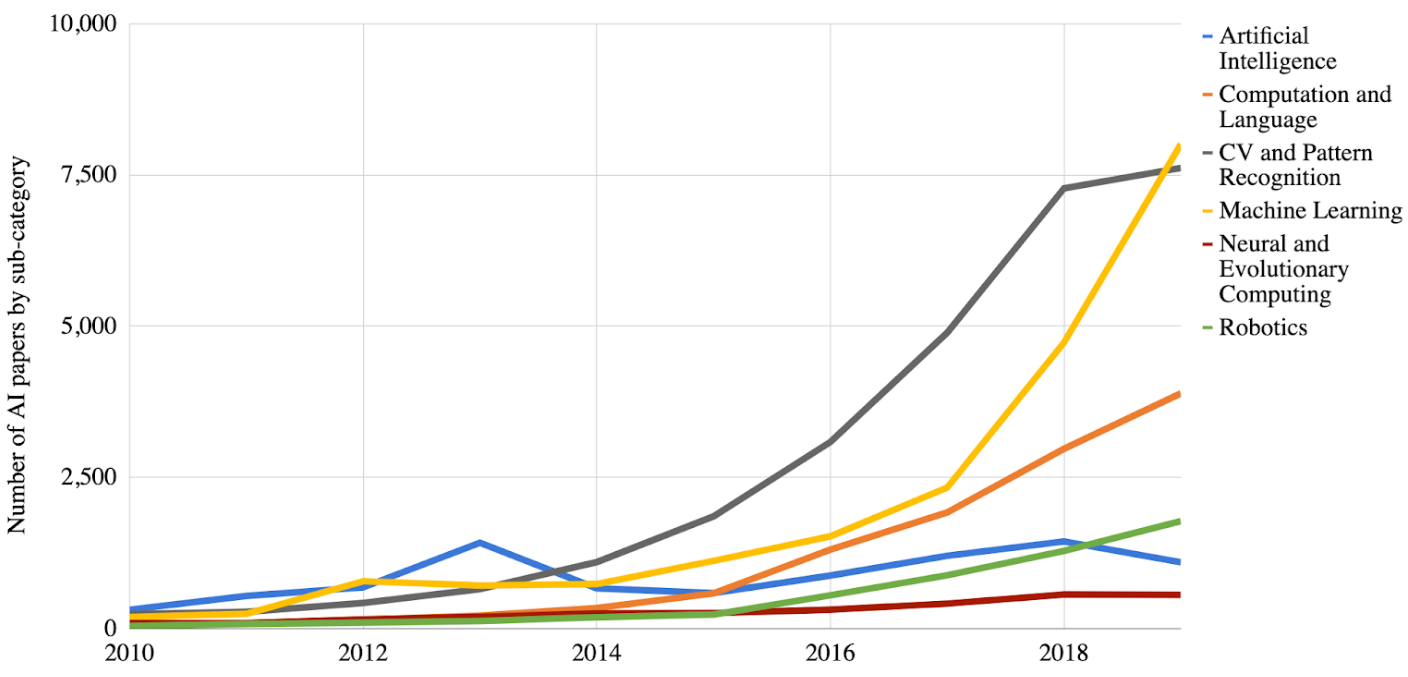
\includegraphics[width=0.8\textwidth]{diagrams/6-cvn/papers.png}
    \caption[papers short]
    {The number of artificial intelligence papers submitted to arXiv, broken down by sub-category.
        Note the particularly large increase in Computer Vision (CV) and pattern recognition
        papers. Figure taken from Ref.\cite{perrault2019}.}
    \label{fig:papers}
\end{figure}

In 2016 the \nova experiment applied a convolutional neural network to the task of classifying the
interaction type of events within their sampling calorimeter detector~\cite{aurisano2016}. Two
views of raw detector events were used as input to train a network based on the popular GoogLeNet
architecture~\cite{szegedy2015}, discussed in section \ref{sec:cvn_theory_conv}. An
improved iteration of the network has since been applied to both the classification of individual
clusters of energy deposits~\cite{psihas2019}, and the regression task of $\nu_{e}$ and $e^{-}$
energy reconstruction~\cite{baldi2019}.

Convolutional neural networks have also been applied to liquid argon time-projection chambers. The
MicroBooNE experiment has shown that in addition to classification tasks, the localisation of
single particles within events is possible~\cite{acciarri2017}. Furthermore, the DUNE
collaboration has designed a network to output both the interaction class and counts of different
particle types in an event~\cite{collaboration2020, abi2020}. This approach is called multi-task
learning, and is discussed in detail within Section.~\ref{sec:cvn_baseline_multi}.

Applications to water Cherenkov detectors have also been made, by both the Daya Bay reactor
experiment~\cite{racah2016} and the KM3NeT/ORCA collaboration~\cite{aiello2020}. Additionally, a
type of generative network known as a `variational autoencoder' has been shown to approximate the
distribution of simulated water Cherenkov data~\cite{abhishek2019}. If further studies prove
successful, this could allow for training on real data to reduce experimental uncertainties and
increase the speed of simulated data generation by many orders of magnitude.

\section{Standard event reconstruction and classification} %%%%%%%%%%%%%%%%%%%%%%%%%%%%%%%%%%%%%%%
\label{sec:cvn_old} %%%%%%%%%%%%%%%%%%%%%%%%%%%%%%%%%%%%%%%%%%%%%%%%%%%%%%%%%%%%%%%%%%%%%%%%%%%%%%

It is essential to outline the standard event reconstruction, and classification methods that have
been used by the \chips project up till now. This is key for two main reasons. Firstly, to add
context when comparing the new convolutional neural network approach, as is done in
Section~\ref{sec:cvn_final_comparison}. Secondly, to highlight the main weaknesses of these
methods, motivating the new technique and making its advantages clear.

A maximum likelihood method based on that implemented by MiniBooNE~\cite{patterson2009} is used
for event reconstruction. Additionally, an artificial neural network built using the TMVA
package~\cite{hocker2007} and using outputs from the reconstruction, is used for event
classification. Both methods are very typical of the `mainstream' approach used by the majority of
water Cherenkov neutrino experiments. A prime example is the fiTQun algorithm developed for the
Super-Kamiokande detector, which is now used for both atmospheric~\cite{jiang2019} and
T2K~\cite{missert2017} analyses.

Due to the limited resources of the \chips collaboration, it is a certainty that both the event
reconstruction and classification do not rep resent an optimal implementation of these methods.
However, it is clear that any possible improvements would be small relative to those introduced by
the convolutional neural network approach. Therefore, for comparisons, it is reasonable to assume
they approximate the maximum performance these approaches can provide.

\subsection{Likelihood based reconstruction} %%%%%%%%%%%%%%%%%%%%%%%%%%%%%%%%%%%%%%%%%%%%%%%%%%%%%
\label{sec:cvn_old_reco} %%%%%%%%%%%%%%%%%%%%%%%%%%%%%%%%%%%%%%%%%%%%%%%%%%%%%%%%%%%%%%%%%%%%%%%%%

The event reconstruction methodology is simple in theory: for a given set of hypothesised tracks,
the number of photoelectrons and the time at which the first of these is recorded for each PMT in
the detector is predicted. By comparing this prediction with the measured hit charges and times
the likelihood that the given track hypothesis produced the measured signals can be calculated.
The parameters that describe the hypothesised tracks are then varied until the negative logarithm
of the likelihood is minimised. Identifying the best-fit parameters for the hypothesis. A brief
description of the procedure is given below, however, for a full description see
Ref.~\cite{blake2016} and in great detail Ref.~\cite{perch2017}.

The first stage of event reconstruction is the effective seeding of tracks that are then used in
the full likelihood fit. The seeding methods aim to provide a good starting point for the
minimisation, both to increase the efficiency of finding the optimal track parameters and also to
avoid a false local minimum from being returned.

Firstly, the PMT hits are sliced in both space and time. Gaps in the time ordering of hits are
used to separate the event into time slices. Each of these then undergoes basic filtering and
clustering to remove outlying hits and ensure only the dominant collections of hits are
considered. Each cleaned slice is then run through simple vertex finding algorithms to estimate
the interaction position and time, as well and the initial track direction.

A circular Hough transform algorithm, traditionally used for water Cherenkov ring finding is then
applied. The voting-based transformation produces as output a space within which rings of PMT hits
exist as single peaks. The track direction values are then further refined using this space, and a
search for smaller peaks is carried out to indicate if multiple particles are likely to be
involved. This process results in a list of seeds with a corresponding score related directly to
the height of the associated peak in Hough transform space.

Each track in a fit hypothesis is made up of a vector of parameters $\vec{x}$, containing the
following:
\begin{itemize}
    \item The track vertex position ($x_{0}$, $y_{0}$, $z_{0}$) and interaction time $t_{0}$.
    \item The initial track direction ($d_{\theta}$, $d_{\phi}$).
    \item The initial kinetic energy of the particle.
    \item The particle type (muon, electron or photon).
\end{itemize}
Additionally, for a photon hypothesis (identical to an electron hypothesis in reality) the
distance between the interaction vertex and the beginning of the electromagnetic shower initiated
by the $\gamma$ is included as a parameter.

All the tracks in the hypothesis are then initialised using those found in the seeding procedure
in descending order of Hough peak height score. As the particle energy is not estimated by the
seeding algorithms, a default value equal to the average particle energy observed in the Monte
Carlo simulation is assigned. Additionally, constraints can be placed on multi-track fits before
the minimisation process begins to reduce the number of free parameters.

For example, in the NC $\pi^{0}$ case, a multi-track two-photon hypothesis is used. Firstly, the
initial parameters for the two photons are assigned from the two highest-scoring seeds. Secondly,
the vertex position for both tracks is constrained to remain the same, and the directions and
energies are set to be constrained by the invariant mass of the $\pi^{0}$.

In it's simplest form the likelihood is a simple product of two terms:
\begin{equation} % LIKELIHOOD EQUATION %
    \mathcal{L}(\vec{x})=\mathcal{L}_{unhit}(\vec{x})\mathcal{L}_{hit}(\vec{x})=
    \prod_{unhit}P_{unhit}(\vec{x})\prod_{hit}P_{charge}(\vec{x})P_{time}(\vec{x}),
    \label{eq:likelihood}
\end{equation}
where the first ($unhit$) gives the likelihood that the hypothesis $\vec{x}$ will not predict a
hit on the PMTs that do not have a measured hit, and the second ($hit$) gives the likelihood that
$\vec{x}$ produces the observed photoelectrons and hit times on the hit PMTs. By considering the
negative logarithm of the likelihood instead, the computation can be simplified into a sum of
logarithms over the PMTs, such that
\begin{equation} % LIKELIHOOD SUM PMTS EQUATION %
    -\log\mathcal{L}(\vec{x})=
    -\sum_{unhit}\log(P_{unhit}(\vec{x}))
    -\sum_{hit}\log(P_{charge}(\vec{x}))
    -\sum_{hit}\log(P_{time}(\vec{x})).
    \label{eq:likelihood_sum}
\end{equation}
This also has the effect of separating the charge (number of photoelectrons) and time prediction
components which can then be dealt with separately computationally. In the actual likelihood
calculation the $P_{unhit}(\vec{x})$ and $P_{charge}(\vec{x})$ components are combined, where the
probability of an unhit PMT is treated as a PMT with observed charge equal to zero.

The Minuit2 algorithm contained within ROOT~\cite{brun1997} is used for the minimisation process.
At each iteration, the charge and hit time predictions are made, and the negative logarithm of the
likelihood is calculated. The track parameters are then varied to minimise the likelihood before
the next iteration. Through a series of stages, fixing and then freeing specific parameters, the
minimisation process converges to the best-fit parameters for the given hypothesis. This process
typically takes two minutes on a standard batch farm computing node.

The charge and hit time predictions and their associated likelihood contributions rely on many
low-level inputs to the reconstruction. These generally describe how Cherenkov light is emitted
from specific particles and then propagates through the detector medium to be detected by the
PMTs. Examples of these inputs include the following:
\begin{itemize}
    \item The number of Cherenkov photons emitted by a particle of specific type and energy.
    \item The fraction of Cherenkov light emitted at each step along a specific particles track
          length.
    \item The angular distribution of Cherenkov photon emission for each type of particle.
    \item The survival probability of photons within the detector medium as a function of
          distance.
    \item A detailed description of the PMT positions and directions within the detector.
    \item The angular efficiency of each PMT relative to the incident photon angle.
    \item The probability of a measured charge given the predicted number of photoelectrons
          (derived from a reversal of the simulation digitisation methodology).
\end{itemize}
The first three are combined into `emission profiles' generated from large samples of the Monte
Carlo simulation, one representation of which is very similar to those shown in
Fig.~\ref{fig:emission_profile}. Additionally, the last listed input is equal to that shown in
Fig.~\ref{fig:digitisation}.

The list above demonstrates a fundamental problem with the likelihood-based approach. It is
heavily reliant on the accuracy of low-level inputs and their associated use in human implemented
software. If a physical process is not dealt with appropriately or overlooked, then the prediction
accuracy of charges and hit times for the PMTs is affected, impacting the performance of finding
the correct best-fit parameters.

The other key flaw of the likelihood-based approach is the requirement of a predefined track
hypothesis. Real events expected within \chips are rarely simple single particle or even
two-particle events. In reality, the majority of events contain multiple final state particles of
various types and in various topologies. The predefinition of a track hypothesis makes it
impossible to implement a generalised approach to event reconstruction where all possible event
types are considered and explored.

\subsection{Event classification}%%%%%%%%%%%%%%%%%%%%%%%%%%%%%%%%%%%%%%%%%%%%%%%%%%%%%%%%%%%%%%%%%
\label{sec:cvn_old_pid} %%%%%%%%%%%%%%%%%%%%%%%%%%%%%%%%%%%%%%%%%%%%%%%%%%%%%%%%%%%%%%%%%%%%%%%%%%

As the reconstruction is based on the calculation of a likelihood (analogous to a
`goodness-of-fit'), the likelihood ratio between different hypotheses can be used for event
classification tasks. It is also found that additional hand-engineered features derived from the
reconstruction outputs have power in classifying the event type.

Two artificial neural networks are used, the first for CC $\nu_{e}$ - CC $\nu_{\mu}$ separation
and the second for CC $\nu_{e}$ - NC separation. Both contain a single hidden layer, with the
number of nodes equal to the number of input parameters plus five. Variables from both a single
$e$ track and single $\mu$ track hypothesis fit to every event are used for both networks, with a
full list of inputs as follows:
\begin{itemize}
    \item The $\Delta\log\mathcal{L}$ between $e$ and $\mu$ hypothesis for both time and
          charge components.
    \item The total number of hit PMTs ($N_{hits}$) and total collected charge.
    \item $\frac{\Delta\log\mathcal{L}_{charge}}{N_{hits}}$.
    \item The fraction of hits inside the central hole, within, and outside the ring for both
          $e$ and $\mu$ hypotheses.
    \item The fraction of predicted charge outside the ring for both $e$ and $\mu$ hypotheses.
    \item The ratio of the total predicted charged to the total measured charge for both $e$
          and $\mu$ hypothesis.
    \item The ratio of the reconstructed energy to the total measured charge.
    \item The reconstructed track direction under the $e$ hypothesis.
    \item The fraction of hits in the downstream half of the detector.
    \item The number of seeds generated by the Hough transform seeding algorithm.
    \item The peak height score of the first and last seeds found by the Hough transform seeding
          algorithm.
\end{itemize}

A sample of CC $\nu_{e}$ and CC $\nu_{\mu}$ beam events characteristic of those expected to be
seen by \chips is used to train the first classifier, and a corresponding sample of CC $\nu_{e}$
and NC events for the second. Both output values can then be used to classify events into separate
samples for further analysis.

The main limitation of this approach is that the input features are restricted to those that have
been imagined (requiring extensive domain knowledge) and then implemented in software. The current
list is almost certainly non exhaustive of all the possible variables and combinations of
variables that can, in theory, be used for discrimination between events. Additionally, any
mistakes in the likelihood-based reconstruction and, therefore, input variables to the artificial
neural networks can lead to incorrect categorisation of events.

\section{The theory of neural networks} %%%%%%%%%%%%%%%%%%%%%%%%%%%%%%%%%%%%%%%%%%%%%%%%%%%%%%%%%%
\label{sec:cvn_theory} %%%%%%%%%%%%%%%%%%%%%%%%%%%%%%%%%%%%%%%%%%%%%%%%%%%%%%%%%%%%%%%%%%%%%%%%%%%

There are many machine learning techniques: linear regression, logistic regression, k-nearest
neighbours, decision trees, random forests, support vector machines, all of which learn to make
predictions about data. However, none have been as successful, especially in recent years, as the
deep neural network. As both the size of datasets and the amount of available computational power
has increased, deep neural networks have proven the most powerful technique for many tasks as they
are well suited to this paradigm.

Here we discuss the application of neural networks for `supervised learning', one of two broad
machine learning categories that is concerned with using labelled example data to train the
algorithm. The other category `unsupervised learning', where the properties the dataset are
inferred without example data is not discussed, however, will be used
Section.~\ref{sec:cvn_explain}.

\subsection{Neural network basics} %%%%%%%%%%%%%%%%%%%%%%%%%%%%%%%%%%%%%%%%%%%%%%%%%%%%%%%%%%%%%%%
\label{sec:cvn_theory_basics} %%%%%%%%%%%%%%%%%%%%%%%%%%%%%%%%%%%%%%%%%%%%%%%%%%%%%%%%%%%%%%%%%%%%

A neural network is a type of supervised learning model inspired by the repeating cell structure
of neurons within our brains. The basic building block of a neural network is a `neuron' which
takes a vector of $k$ inputs $\vec{x} = (x_{1}, x_{2},\dots,x_{k})$ and outputs a scalar
$a(\vec{x})$. The neurons are arranged into layers, with input of one layer being the output from
the previous layer. The first layer is commonly referred to as the input layer, the middle layers
as `hidden layers', and the final layer as the output layer, as illustrated in
Fig.~\ref{fig:network}. In general, this simple neural network structure is referred to as
`fully-connected' as all the neurons in each layer have connections to all the neurons in the
previous and following layers.

\begin{figure} % BASIC NETWORK DIAGRAM %
    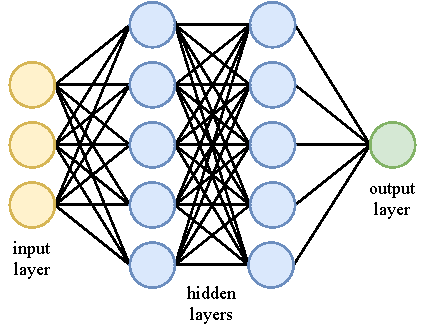
\includegraphics[width=0.6\textwidth]{diagrams/6-cvn/network.pdf}
    \caption[Illustration of a simple neural network]
    {Illustration of a simple neural network. There is a single input layer (yellow), two hidden
        layers (blue), and an output layer (green). Each node corresponds to a `neuron' except for
        the input layer.}
    \label{fig:network}
\end{figure}

Input variables (traditionally hand-engineered features extracted from the raw data) are passed
into the network via the input layer. Any number of hidden layers containing any number of neurons
can then follow. The neurons contained within these layers are `trained' so that collectively
their $a(\vec{x})$ functions solve the problem at hand. For a regression task, the output layer
outputs a continuous decimal value. Otherwise, for a classification task, a probability value
between zero and one is output for each class. The forward passing of information from one layer
to the next is why neural networks can also be referred to as `feed-forward graphs'.

For a neuron $i$, $a_{i}(\vec{x})$ can be decomposed into a linear operation, specific to the
neuron, followed by a non-linear operation, which is the same across all neurons. The linear
operation consists of the dot product of the input vector $\vec{x}$ with a vector of weights
$\vec{w}^{(i)} = (w_{1}^{(i)}, w_{2}^{(i)},\dots,w_{k}^{(i)})$, which weight the relative
importance of the inputs, plus a bias term $b^{(i)}$:
\begin{equation} % NETWORK BASIC EQUATION %
    z^{(i)}=\vec{w}^{(i)}\cdot\vec{x}+b^{(i)}.
    \label{eq:network}
\end{equation}
After applying the non-linear operation $\sigma_{i}$, commonly referred to as the `activation
function' the final output from the neuron can be written as
\begin{equation} % NETWORK ACTIVATION EQUATION %
    a_{i}(\vec{x})=\sigma_{i}(z^{(i)}).
    \label{eq:activation}
\end{equation}

Traditionally, a step-function (for networks called perceptrons) was used for the activation
function. However, as is shown in Section.~\ref{sec:cvn_theory_training}, a non-zero gradient
(only valid at $x=0$ for a step-function) is required for the practical training of neural
networks. In fact, the choice of activation function can greatly affect how the network trains and
performs.

Therefore, common choices have been the hyperbolic tangent and the sigmoid function, primarily
because they are bounded and differentiable at all points. Recently, the ReLU and other similar
functions have become popular, especially for convolutional neural networks. This is mainly due to
them avoiding the problem of `vanishing gradients' caused by the saturation of the tanh and
sigmoid functions at large values of $x$. All of these functions are shown in
Fig.~\ref{fig:activations}.

\begin{figure} % ACTIVATIONS DIAGRAM %
    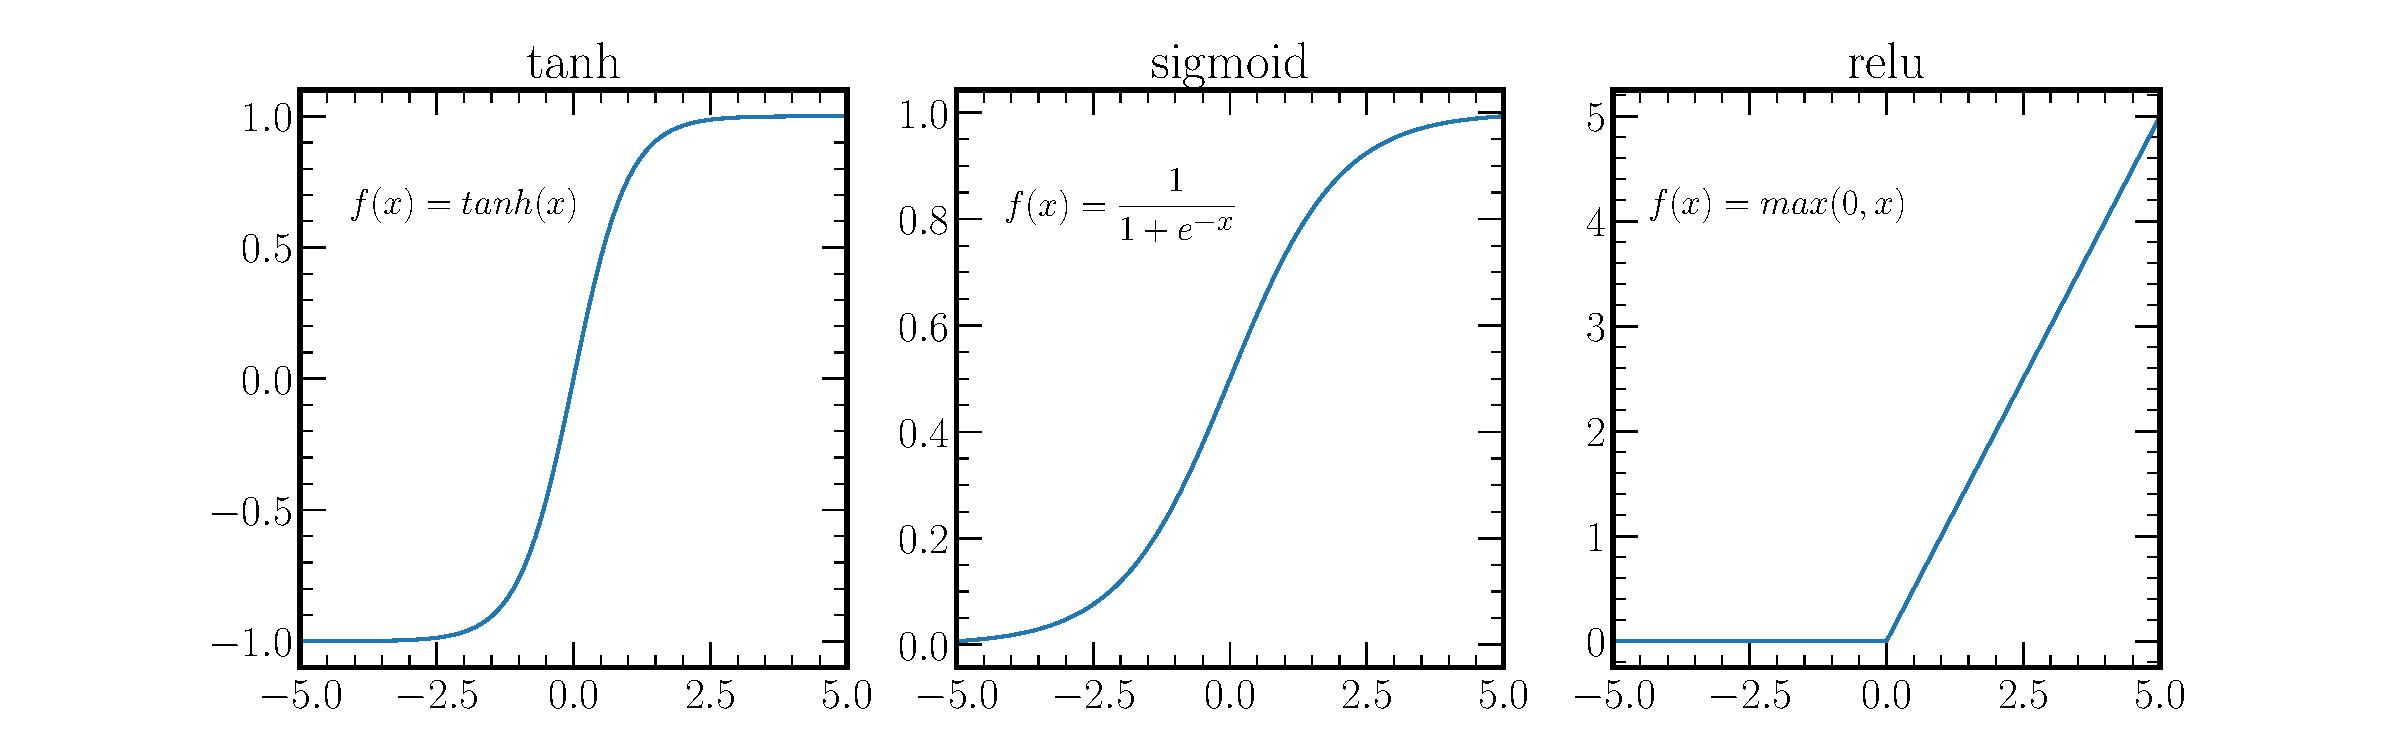
\includegraphics[width=\textwidth]{diagrams/6-cvn/activations.pdf}
    \caption[Common non-linear activation functions.]
    {Common non-linear activation functions used for the neurons within neural networks.}
    \label{fig:activations}
\end{figure}

\subsection{Training neural networks} %%%%%%%%%%%%%%%%%%%%%%%%%%%%%%%%%%%%%%%%%%%%%%%%%%%%%%%%%%%%
\label{sec:cvn_theory_training} %%%%%%%%%%%%%%%%%%%%%%%%%%%%%%%%%%%%%%%%%%%%%%%%%%%%%%%%%%%%%%%%%%

The process of supervised training of a neural network uses labelled data to iteratively find the
optimal weights and biases (network parameters) that maximise the network performance. In order to
quantify the performance, we must define a loss function $E(\vec{w})$, where $\vec{w}$ is the
vector of network parameters, describing the difference between the network output and the true
label. For a given input data point $(\vec{x}_{i}, y_{i})$, where $\vec{x}_{i}$ are the input
parameters and $y_{i}$ is the known truth label, the network generates an output
$\hat{y}_{i}(\vec{w})$. Using this notation, we can then construct loss functions suitable for
different tasks.

In the case of a simple binary classification task, the most commonly used function is the
cross-entropy:
\begin{equation} % BINARY CROSS-ENTROPY EQUATION %
    E(\vec{w})=
    -\displaystyle\sum_{i=1}^{n}y_{i}\log\hat{y}_{i}(\vec{w})+
    (1-y_{i})\log[1-\hat{y}_{i}(\vec{w})],
    \label{eq:binary_cross_entropy}
\end{equation}
where the number of data points is given by $n$. For a classification task where the number of
classes is greater than two $y$ can take on $M$ values. In this case we redefine each data point
so that $y$ is instead a vector $y_{im}$ such that
\begin{equation} % ONE-HOT EQUATION %
    y_{im}=
    \begin{cases}
        1 & \text{if $y_{i}=m$} \\
        0 & \text{otherwise.}   \\
    \end{cases}
\end{equation}
This is commonly named a `one-hot' vector. The cross-entropy then becomes
\begin{equation} % CATEGORICAL CROSS-ENTROPY EQUATION %
    E(\vec{w})=
    -\displaystyle\sum_{i=1}^{n}\displaystyle\sum_{m=0}^{M-1}y_{im}\log\hat{y}_{im}
    (\vec{w})+(1-y_{im})\log[1-\hat{y}_{im}(\vec{w})].
    \label{eq:categorical_cross_entropy}
\end{equation}
For a regression task predicting a continuous output variable, the mean-squared error is most
often used as the loss function:
\begin{equation} % MEAN-SQUARED ERROR LOSS EQUATION %
    E(\vec{w})=
    \frac{1}{n}\displaystyle\sum_{i=1}^{n}(y_{i}-
    \hat{y}_{i}(\vec{w}))^{2}.
    \label{eq:mse}
\end{equation}

To find the optimal network parameters for the given task we can iteratively minimise the loss
function until it converges to its minimum (or in reality a local minimum that performs well).
This is done by updating the network parameters at each iteration $t$ to move in the direction of
the gradient of the loss function using an update rule:
\begin{equation} % UPDATE EQUATION %
    \vec{w}_{t+1}=\vec{w}_{t}-\eta_{t}\nabla_{\vec{w}}E(\vec{w}),
    \label{eq:update_rule}
\end{equation}
where $\eta_{t}$ is the `learning rate' which determines the size of the step that is taken at
each iteration. This methodology is known as `gradient descent' and is illustrated in
Fig.~\ref{fig:gradient_descent}.

\begin{figure} % GRADIENT DESCENT DIAGRAM %
    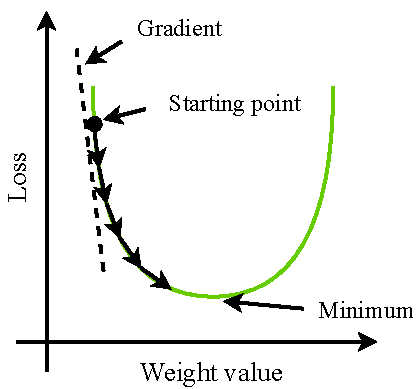
\includegraphics[width=0.5\textwidth]{diagrams/6-cvn/gradient_descent.pdf}
    \caption[Illustration of the gradient descent process.]
    {Simplified illustration of the gradient descent process. Shown is the case for a loss
        function dependent on a single weight.}
    \label{fig:gradient_descent}
\end{figure}

Therefore, in order to use gradient descent, we require that the gradient of the loss function
with respect to the parameters of the network can be calculated. Doing this for each parameter at
every iteration would render neural networks impossible to use due to the vast computational
requirements. Instead, an innovative application of the chain rule in an algorithm called
`backpropagation' (backprop) is used~\cite{werbos1974}. Here we follow the derivation of the four
main equations of backpropagation from Ref.~\cite{mehta2019}.

For a network containing $L$ layers, we can index the individual layers using $l=1,\dots,L$. The
weight associated with the connection between the $k$-th neuron in layer $l-1$ and the $j$-th
neuron in layer $l$ can be denoted as $w^{l}_{jk}$. The bias of the layer $l$ neuron is written as
$b^{l}_{j}$. The activation of the $j$-th neuron in layer $l$ is then related to the outputs from
the previous layer by
\begin{equation} % PREVIOUS LAYER EQUATION %
    a^{l}_{j}=\sigma(z^{l}_{j})=\sigma\left(\sum_{k}w^{l}_{jk}a^{l-1}_{k}+b^{l}_{j}\right).
    \label{eq:feedforward}
\end{equation}

The change in the loss function with respect to the linear weighted sum $z^{l}_{j}$ of the $j$-th
neuron in the last layer $L$ can be used to define the error:
\begin{equation} % PREVIOUS LAYER EQUATION %
    \Delta^{L}_{j}=\frac{\partial E}{\partial z^{L}_{j}}.
\end{equation}
Similarly the error on any neuron $j$ in any layer $l$ is given by
\begin{equation} % BACKPROP EQUATION 1 %
    \Delta^{l}_{j}=\frac{\partial E}{\partial z^{l}_{j}}=\frac{\partial E}{\partial a^{l}_{j}}
    \sigma '(z^{l}_{j}),
    \label{eq:backprop_1}
\end{equation}
with $\sigma '$ denoting the derivative of the non-linear activation function. As $\partial
    b^{l}_{j}/\partial z^{l}_{j}=1$, the error can also be viewed as the partial derivative of the
loss function with respect to the bias:
\begin{equation} % BACKPROP EQUATION 2 %
    \Delta^{l}_{j}=\frac{\partial E}{\partial z^{l}_{j}}
    =\frac{\partial E}{\partial b^{l}_{j}}\frac{\partial b^{l}_{j}}{\partial z^{l}_{j}}
    =\frac{\partial E}{\partial b^{l}_{j}}.
    \label{eq:backprop_2}
\end{equation}

Using the chain rule and the fact that the error on neurons in layer $l$ only depends on the
activation of neurons in the following layer $l+1$, we can write
\begin{align} % BACKPROP EQUATION 3 %
    \begin{split}
        \Delta^{l}_{j} &=\frac{\partial E}{\partial z^{l}_{j}}
        =\sum_{k}\frac{\partial E}{\partial z^{l+1}_{k}}
        \frac{\partial z^{l+1}_{k}}{\partial z^{l}_{j}} \\
        &=\sum_{k}\Delta^{l+1}_{k}\frac{\partial z^{l+1}_{k}}{\partial z^{l}_{j}} \\
        &=\left(\sum_{k}\Delta^{l+1}_{k}w^{l+1}_{kj}\right)\sigma '(z^{l}_{j}).
    \end{split}
    \label{eq:backprop_3}
\end{align}
Additionally, the differential of the cost function with respect to the weight $w^{l}_{jk}$ can be
written as
\begin{equation} % BACKPROP EQUATION 4 %
    \frac{\partial E}{\partial w^{l}_{jk}}
    =\frac{\partial E}{\partial z^{l}_{j}}\frac{\partial z^{l}_{j}}{\partial w^{l}_{jk}}
    =\Delta^{l}_{j}a^{l-1}_{k}.
    \label{eq:backprop_4}
\end{equation}

The full backpropagation algorithm then proceeds as follows:
\begin{enumerate}
    \item After calculating the activations $a^{1}_{j}$ for all neurons in the input layer, use
          the feed-forward architecture of the network to calculate all activations at every layer
          using Eq.~\ref{eq:feedforward}.
    \item Use Eq.~\ref{eq:backprop_1} to calculate the error of the top layer neurons. Both the
          derivative of the loss function and the activation function is required for this step.
    \item Use Eq.~\ref{eq:backprop_2} to `backpropagate' the error through the network from the
          top layer to the input layer to find all $\Delta^{l}_{j}$ values.
    \item Calculate the gradients for all the weights and biases using Eq.~\ref{eq:backprop_3} and
          Eq.~\ref{eq:backprop_4}.
\end{enumerate}
As can be seen a single `forward' pass to find the activations and a single `backward' pass
propagating the error is all that's required to calculate the gradients for all weights and
biases within the network. This incredibly efficient procedure allows for the use of gradient
descent to train neural networks.

\subsection{Convolutional neural networks} %%%%%%%%%%%%%%%%%%%%%%%%%%%%%%%%%%%%%%%%%%%%%%%%%%%%%%%
\label{sec:cvn_theory_conv} %%%%%%%%%%%%%%%%%%%%%%%%%%%%%%%%%%%%%%%%%%%%%%%%%%%%%%%%%%%%%%%%%%%%%%

The broad category of `deep learning' covers multiple neural network techniques spanning a range
of application fields such as computer vision, speech recognition and natural language processing.
By stacking many layers on top of each other into a `deep' network, these methods offer increased
problem-solving capacity by allowing higher-order non-linear functions to form. Therefore, instead
of requiring hand-engineered features as input, these techniques work to extract the most
important features from raw data. Here we outline just the technique used in this work; the
convolutional neural network (CNN).

At their core, a CNN makes use of a mathematical operation called convolution, which either
entirely or in part replaces the simple vector multiplication seen in fully-connected networks as
introduced in Section~\ref{sec:cvn_theory_basics}. This change makes CNNs incredibly powerful for
applications using grid-like data such as computer vision tasks.

Using standard CNN terminology, the discrete convolution between the input $x$ and the kernel $w$
is given by
\begin{equation}
    f_{i}=(x*w)_{i}=\sum^{\infty}_{j=-\infty}x_{j}w_{i-j},
\end{equation}
where the output $f$ is commonly referred to as the feature map. In typical applications, the
input is a two-dimensional array of input values $X$. Therefore, both the kernel $W$ and the
resulting feature map $F$ also become two-dimensional. In this case the convolution operation
becomes
\begin{equation}
    F_{i}=(X*W)_{i,j}=\sum_{m}\sum_{n}X_{i+m,j+n}W_{m,n},
    \label{eq:conv}
\end{equation}
where the infinite sum has been replaced with a discrete sum over two-dimensional elements.
Normally the output feature map is then passed through a non-linear activation function. Analogous
to the simple neural network weights $\vec{w}$ first described in Eq.~\ref{eq:network}, the
elements of $W_{m,n}$ can be trained to maximise the network performance (minimise the loss).

To illustrate this operation Fig.~\ref{fig:conv_input} gives examples of a $4 \times 4$ input grid
and a $3 \times 3$ kernel. The output feature map is generated by sliding the kernel across both
dimensions of the input grid, summing the products of all associated elements at each step
according to Eq.~\ref{eq:conv}, as shown in Fig.~\ref{fig:conv_operation}.

\begin{figure} % CONV INPUTS DIAGRAM %
    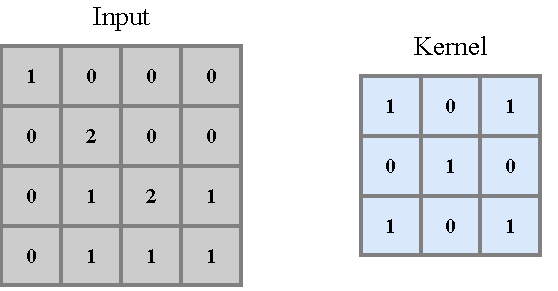
\includegraphics[width=0.6\textwidth]{diagrams/6-cvn/conv_input.pdf}
    \caption[Example of an input grid and kernel.]
    {Example of an input grid (left) and kernel (right). The specific kernel shown is sensitive to
        x-shaped features}
    \label{fig:conv_input}
\end{figure}

\begin{figure} % CONV OPERATION DIAGRAM %
    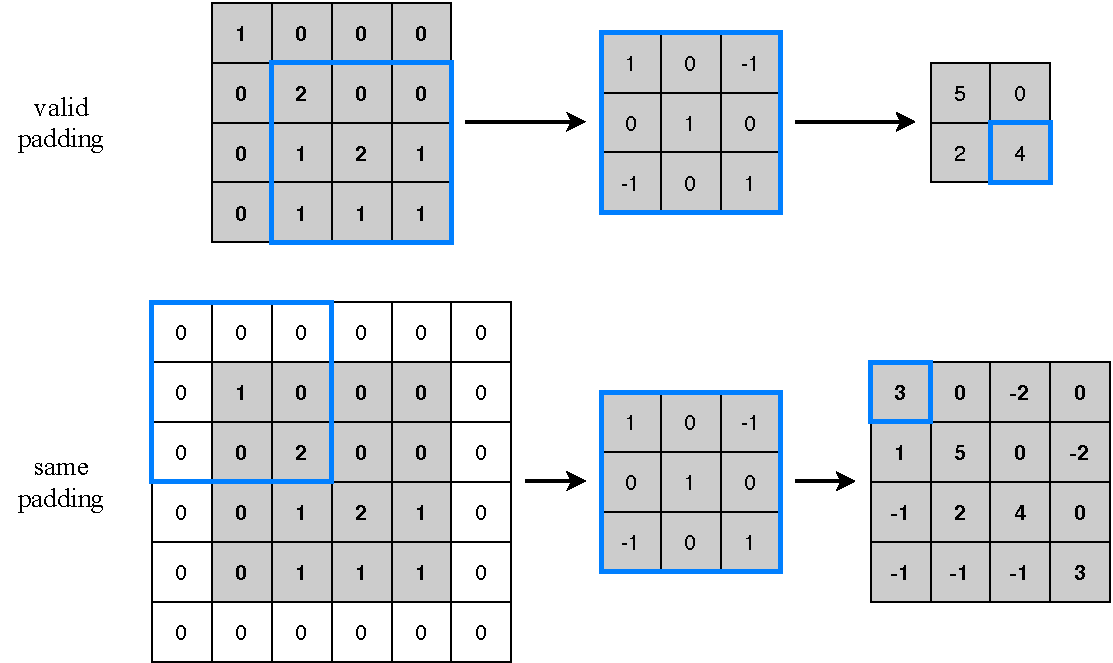
\includegraphics[width=0.8\textwidth]{diagrams/6-cvn/conv_operation.pdf}
    \caption[Example of convolutional operation.]
    {Example of a $\mathrm{stride}=1$ convolutional operation involving the input grid and kernel
        from Fig.~\ref{fig:conv_input}. Both the operation for the case of `valid' (top) and
        `same' (bottom) padding is shown. The blue square in the top-left of the output feature
        maps indicates the output generated from the specific operation shown.}
    \label{fig:conv_operation}
\end{figure}

Two additional parameters that affect the output size of the feature map are also introduced in
Fig.~\ref{fig:conv_operation}. The `stride' and the `padding'. The stride governs how far the
kernel moves at each step while the padding decides if the input grid is padded with zeros around
its border. If $L$ is the size of the input (both height and width) and $K$ is the kernel size,
the output feature map size $O$ is given by
\begin{equation}
    O=\frac{(L-K+2P)}{S}+1,
    \label{eq:conv_size}
\end{equation}
where $S$ is the stride, and $P$ is the amount of zero padding.

The other key operation used in CNNs is pooling. To reduce the number of network parameters which
is typically high for CNNs, pooling layers coarse-grain the spatial information of the input via
down-sampling. `Max pooling' or `average pooling' are the two common ways this is achieved. In
both cases, the input is first divided into rectangular regions, and then either the maximum or
average value of the region is used as output, for max and average pooling respectively. This is
illustrated in Fig.\ref{fig:pooling}.

\begin{figure} % POOLING DIAGRAM %
    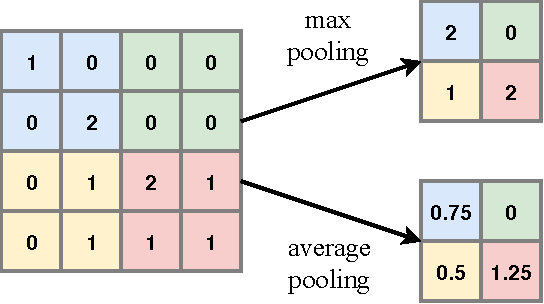
\includegraphics[width=0.6\textwidth]{diagrams/6-cvn/pooling.pdf}
    \caption[Example of pooling operation.]
    {Example of both a max and average $2 \times 2$ pooling operation with $\mathrm{stride}=2$.}
    \label{fig:pooling}
\end{figure}

Taking inspiration from how neurons behave in the visual cortex of animals~\cite{lecun2015}, small
kernels are generally used that only scan over a small spatial patch of the input at any one time.
When combined with the loss of absolute position information that pooling produces, it highlights
a key feature of CNNs. They exhibit translational invariance and respect the local structure
contained within the input. In simpler terms, they do not care wherein the input image a
particular feature exists, just that it exists.

\subsubsection*{CNN architectures}

In 2012 the AlexNet CNN lowered the error rate of the ubiquitous ImageNet classification
task~\cite{deng2009} from 28\% to 16\%~\cite{krizhevsky2012}. Since this breakthrough, the
standard CNN has adopted the same architecture. Multiple convolutional layers are stacked on top
of each other, periodically interspersed with pooling layers. Once the output feature map size no
longer allows for additional pooling, one or more fully-connected layers are added before the final
output layer, as shown in Fig.~\ref{fig:conv_diagram}.

\begin{figure} % CONV DIAGRAM %
    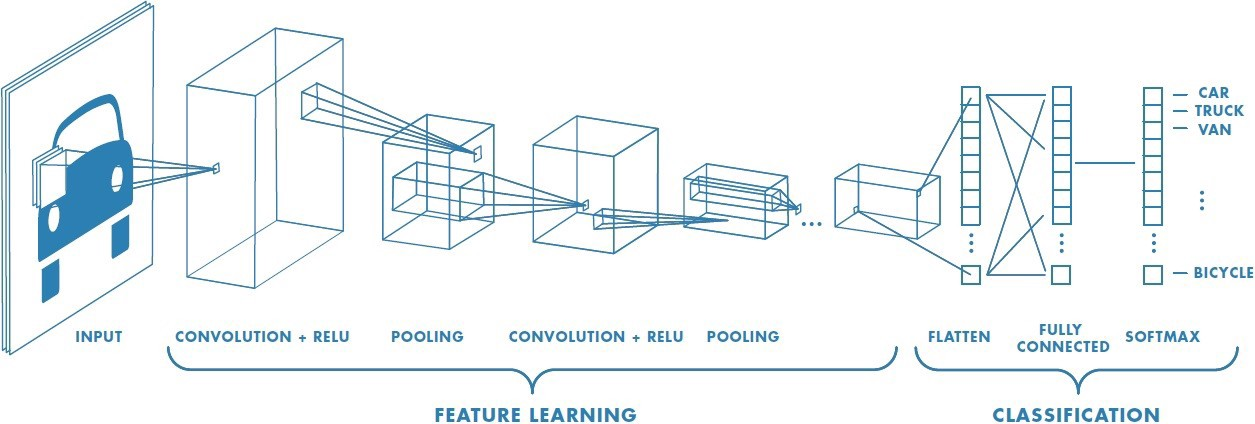
\includegraphics[width=\textwidth]{diagrams/6-cvn/conv_diagram.jpeg}
    \caption[Typical CNN architecture]
    {Illustration of a typical CNN architecture, containing convolutional, pooling and
        fully-connected layers before the final output layer.}
    \label{fig:conv_diagram}
\end{figure}

Led by research teams at the technology giants, improvements upon this standard architecture have
been made. Initially this involved the addition of extra convolutional layers to form a deeper
network as VGG did in 2014~\cite{simonyan2014}. Separately, the `inception module' introduced by
GoogLeNet~\cite{szegedy2015} the same year allowed for different scales of features to be explored
using the concept of a `network within a network'.

As the size of CNNs increased it was found that the gradients on the lower layers of the network
were found to decrease. This sometimes had the effect of the gradient `vanishing' from these
layers preventing learning. To counter this problem ResNet~\cite{he2016_original, he2016_improved}
introduced residual connections, skipping specific layers and allowing for a large gradient to
reach the affected lower layers during backpropagation. Recently the inception module and ResNet
ideas have been combined~\cite{szegedy2016}, and there has been a significant push for efficient
rather than just deeper networks~\cite{sandler2018,tan2019}. The repeating layout of layers that
form the above networks, often referred to as `blocks', are shown in Fig.~\ref{fig:blocks}.

\begin{figure} % BLOCKS DIAGRAM %
    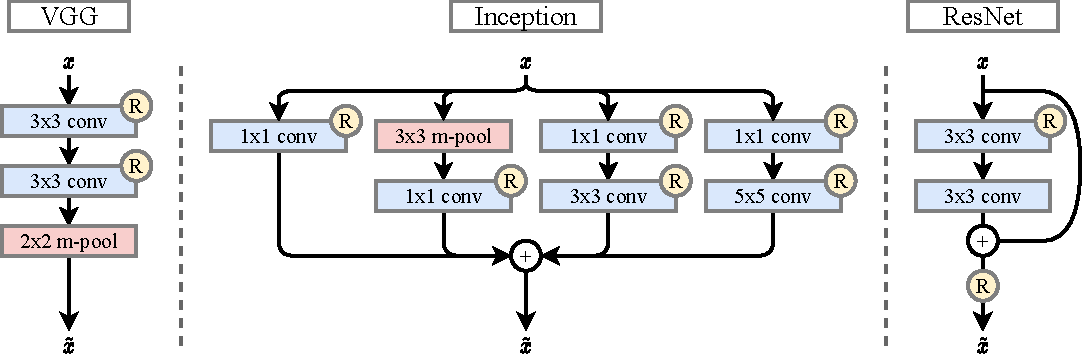
\includegraphics[width=\textwidth]{diagrams/6-cvn/blocks.pdf}
    \caption[Common CNN architecture blocks]
    {Common blocks used within CNN architectures, taking $x$ as input and producing $\tilde{x}$ as
        output through operations whose flow is outlined via the arrows. The blue and red boxes
        represent convolutional and pooling layers respectively, with the size of the operation
        shown. The circular yellow $R$ indicates the use of the ReLU activation function.}
    \label{fig:blocks}
\end{figure}

\subsection{Regularisation} %%%%%%%%%%%%%%%%%%%%%%%%%%%%%%%%%%%%%%%%%%%%%%%%%%%%%%%%%%%%%%%%%%%%%%
\label{sec:cvn_theory_reg} %%%%%%%%%%%%%%%%%%%%%%%%%%%%%%%%%%%%%%%%%%%%%%%%%%%%%%%%%%%%%%%%%%%%%%%

A key challenge for supervised machine learning techniques is ensuring the algorithm can
generalise to new previously unseen datasets. This can be difficult when for a deep neural network
containing millions of trainable parameters, it can become easy for the network to learn the
specific features and noise of the training dataset. This process is called `overfitting' and is
common when training convolutional neural networks. Methods used within this work to prevent this
from happening are outlined below, all of which are commonly referred to as `regularisation'
techniques.

\subsubsection*{Stochastic Gradient Descent}

The process outlined so far of updating the network weights at each training iteration using the
gradient calculated over the full dataset is called `batch training'. It is instead much more
common to calculate an approximation to the gradient at each iteration using a `minibatch' of the
full dataset. This is done by considering just a subset of the training data with a size commonly
referred to as the `batch size' and typically equal to a power of two for computational reasons.

This modification to standard gradient descent is called stochastic gradient descent as it
introduces stochasticity to the training process, and has two main advantages. Firstly the
computational speed of each iteration is significantly reduced, and crucially the memory
requirements lowered. Secondly, the additional noise introduced decreases the chance that the
minimisation will get stuck in a local minimum suited to overfitting the training dataset.

\subsubsection*{Early stopping}

Early stopping is a simple procedure which prevents the inevitable overfitting process from
affecting the final generalised performance of the network. During training, the training dataset
is commonly iterated over multiple times, with each iteration called an `epoch'. By evaluating the
error on an independent `validation' dataset at the end of each epoch, the point at which
overfitting begins can be determined, as shown in Fig.~\ref{fig:early_stopping}. At this point,
the training is stopped to return the best possible generalised model. In practice, it is common
only to stop training after $n$ number of epochs have passed with no improvement.

\begin{figure} % EARLY STOPPING DIAGRAM %
    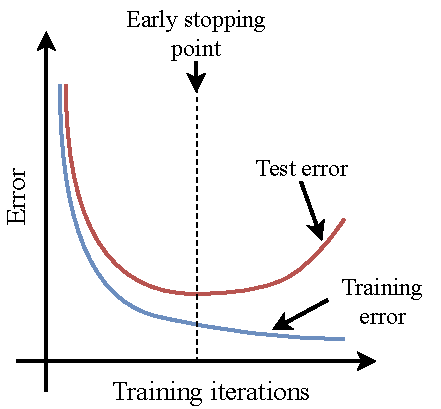
\includegraphics[width=0.5\textwidth]{diagrams/6-cvn/early_stopping.pdf}
    \caption[Illustration of the early stopping procedure.]
    {Illustration of the early stopping procedure. Initially both the training and test error
        decreases, but, at some point the test error will start to increase due to overfitting, at
        this point the training is stopped.}
    \label{fig:early_stopping}
\end{figure}

\subsubsection*{Batch normalisation}

The training of a neural network is found to work best when the inputs of each neuron are centred
on zero with respect to the bias of the neuron. This is because neuron input values can cause
saturation of the activation function and subsequent `vanishing' of the associated gradient,
reducing the ability of the network to learn. To counter this, Batch
Normalisation~\cite{ioffe2015} introduces layers that standardise the inputs using the mean and
variance calculated over each minibatch. This not only speeds up training by preventing the
`vanishing' of gradients but also reduces overfitting by again using the stochasticity of the
minibatch.

\subsubsection*{Dropout}

Dropout is another simple technique to reduce the overfitting of training data~\cite{hinton2012}.
At each training iteration, each neuron has a probability $p$ to be `dropped-out' and ignored in
the iterations calculations. This is illustrated in \ref{fig:dropout}. By ignoring a subset of the
neurons at each iteration it makes it harder for the network to form the particularly strong
connections between neurons that are usually responsible for overfitting, allowing for a better
generalisation.

\begin{figure} % DROPOUT DIAGRAM %
    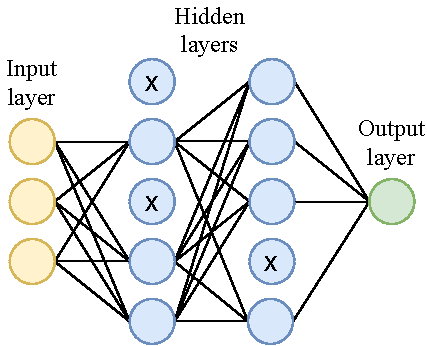
\includegraphics[width=0.6\textwidth]{diagrams/6-cvn/dropout.pdf}
    \caption[Illustration of dropout.]
    {Example of dropout applied to the network shown in Fig.~\ref{fig:network}. Neurons are
        randomly `dropped out' and not considered at each training step. This reduces the strong
        correlations between neurons that can lead to overfitting.}
    \label{fig:dropout}
\end{figure}

\section{A baseline implementation for CHIPS} %%%%%%%%%%%%%%%%%%%%%%%%%%%%%%%%%%%%%%%%%%%%%%%%%%%%
\label{sec:cvn_baseline} %%%%%%%%%%%%%%%%%%%%%%%%%%%%%%%%%%%%%%%%%%%%%%%%%%%%%%%%%%%%%%%%%%%%%%%%%

The output from a water Cherenkov neutrino detector is effectively a simple image of each event
where the number of photoelectrons and hit times for each PMT are known.

- We need a grid-like topology

-Water Cherenkov detectors generate essentially an `image' of the neutrino interaction and
therefore they are well suited to use things from computer vision.
- Many HEP problems including water cherenkov detectors essentially result in an 'image' of an
event, which are well suited to these tools.
- CNNs have been widely applied in various computer vision tasks to solve image recognition and
analysis problems.

\subsection{Model evaluation} %%%%%%%%%%%%%%%%%%%%%%%%%%%%%%%%%%%%%%%%%%%%%%%%%%%%%%%%%%%%%%%%%%%%
\label{sec:cvn_baseline_soft} %%%%%%%%%%%%%%%%%%%%%%%%%%%%%%%%%%%%%%%%%%%%%%%%%%%%%%%%%%%%%%%%%%%%

\begin{figure} % OSC FLUXES DIAGRAM %
    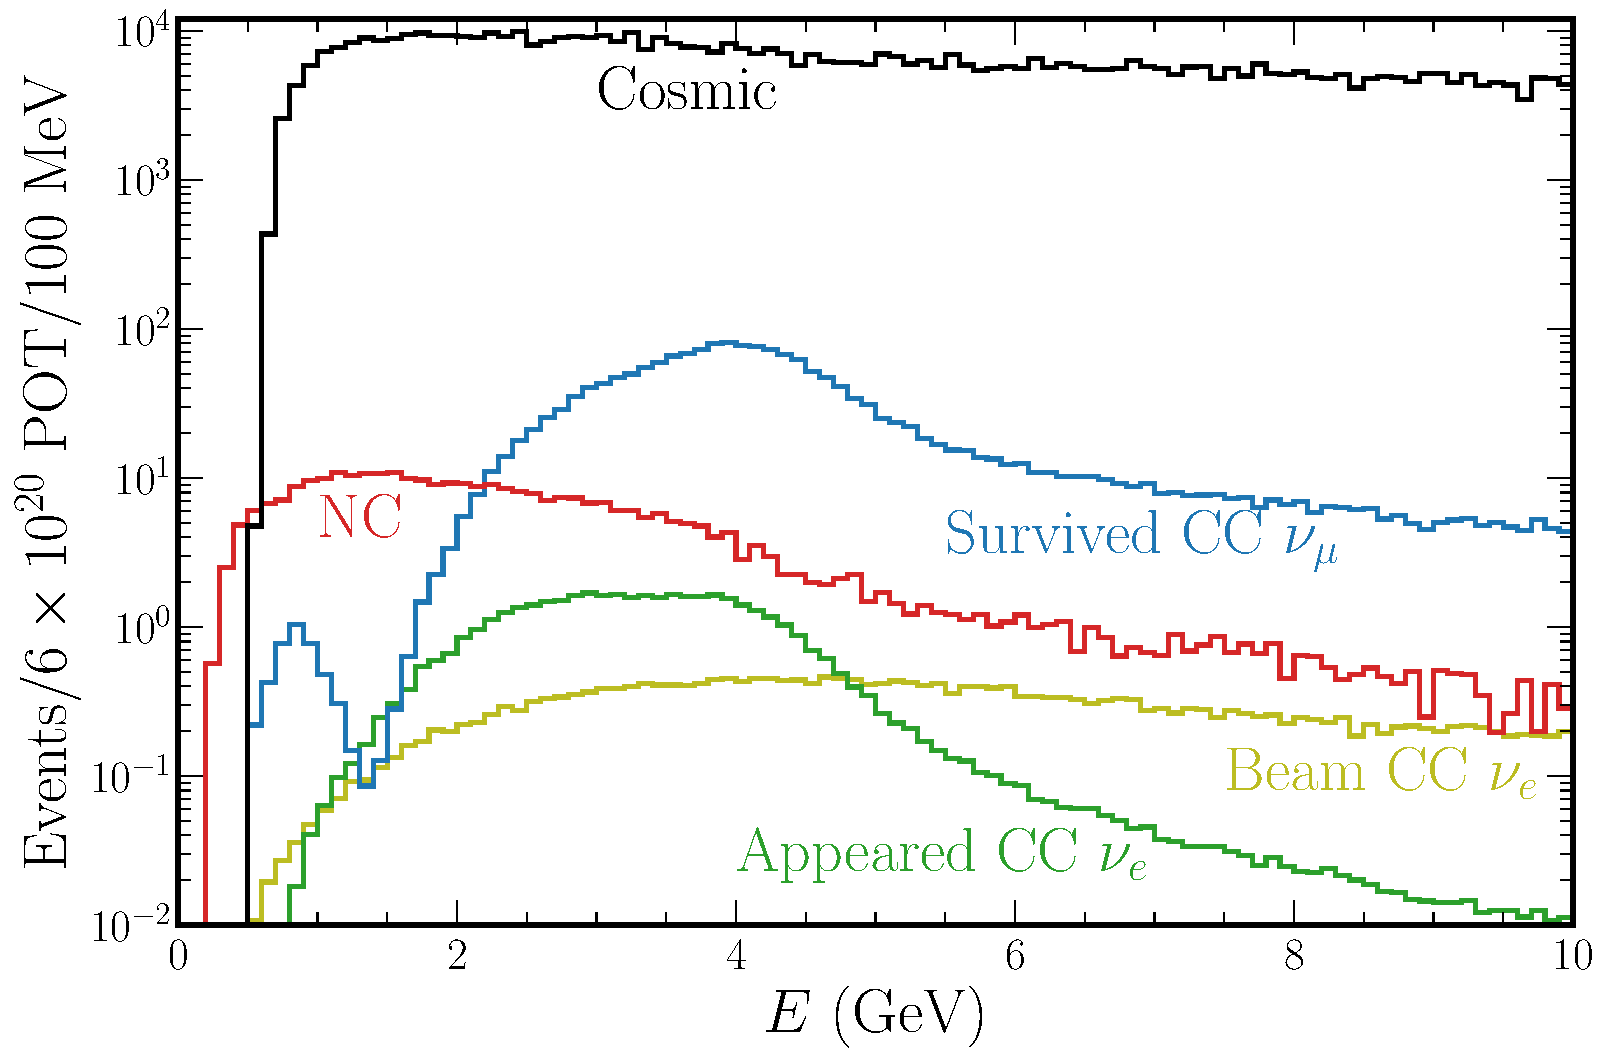
\includegraphics[width=0.8\textwidth]{diagrams/6-cvn/chipsnet/explore_osc_fluxes.pdf}
    \caption[explore osc fluxes short]
    {explore osc fluxes long}
    \label{fig:explore_osc_fluxes}
\end{figure}

\begin{figure} % STACK INT TYPES DIAGRAM %
    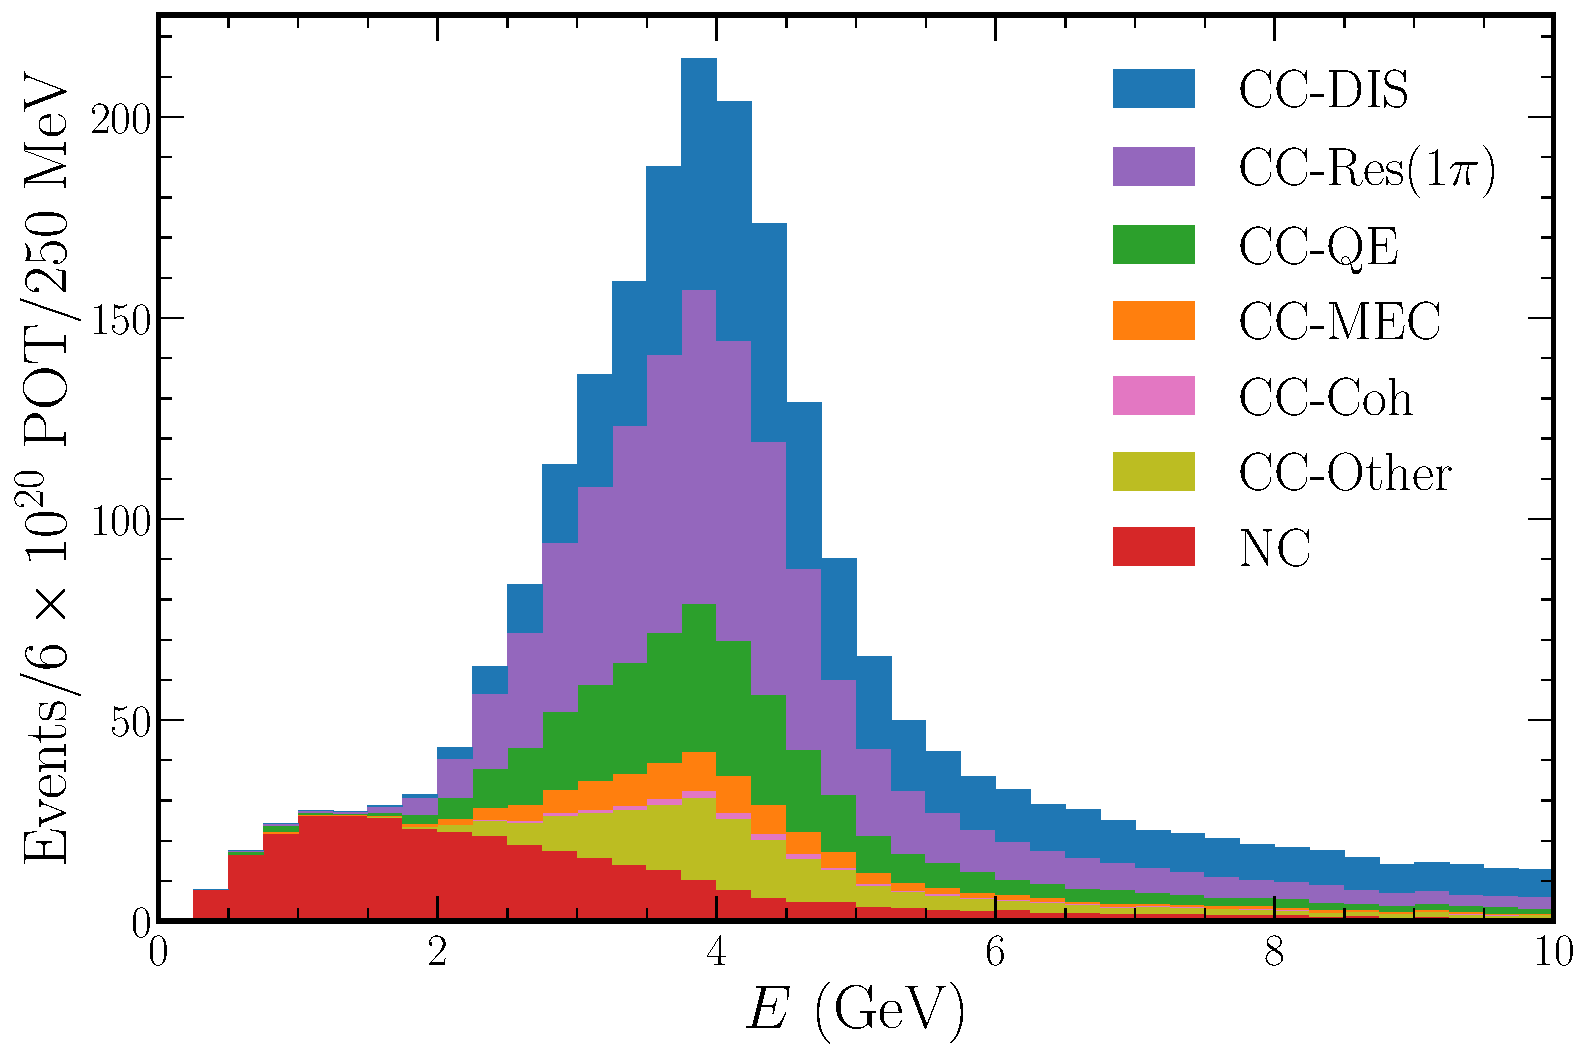
\includegraphics[width=0.8\textwidth]{diagrams/6-cvn/chipsnet/explore_stacked_int_types.pdf}
    \caption[explore stacked int types short]
    {explore stacked int types long}
    \label{fig:explore_stacked_int_types}
\end{figure}

\begin{figure} % SIMPLE CUTS DIAGRAM %
    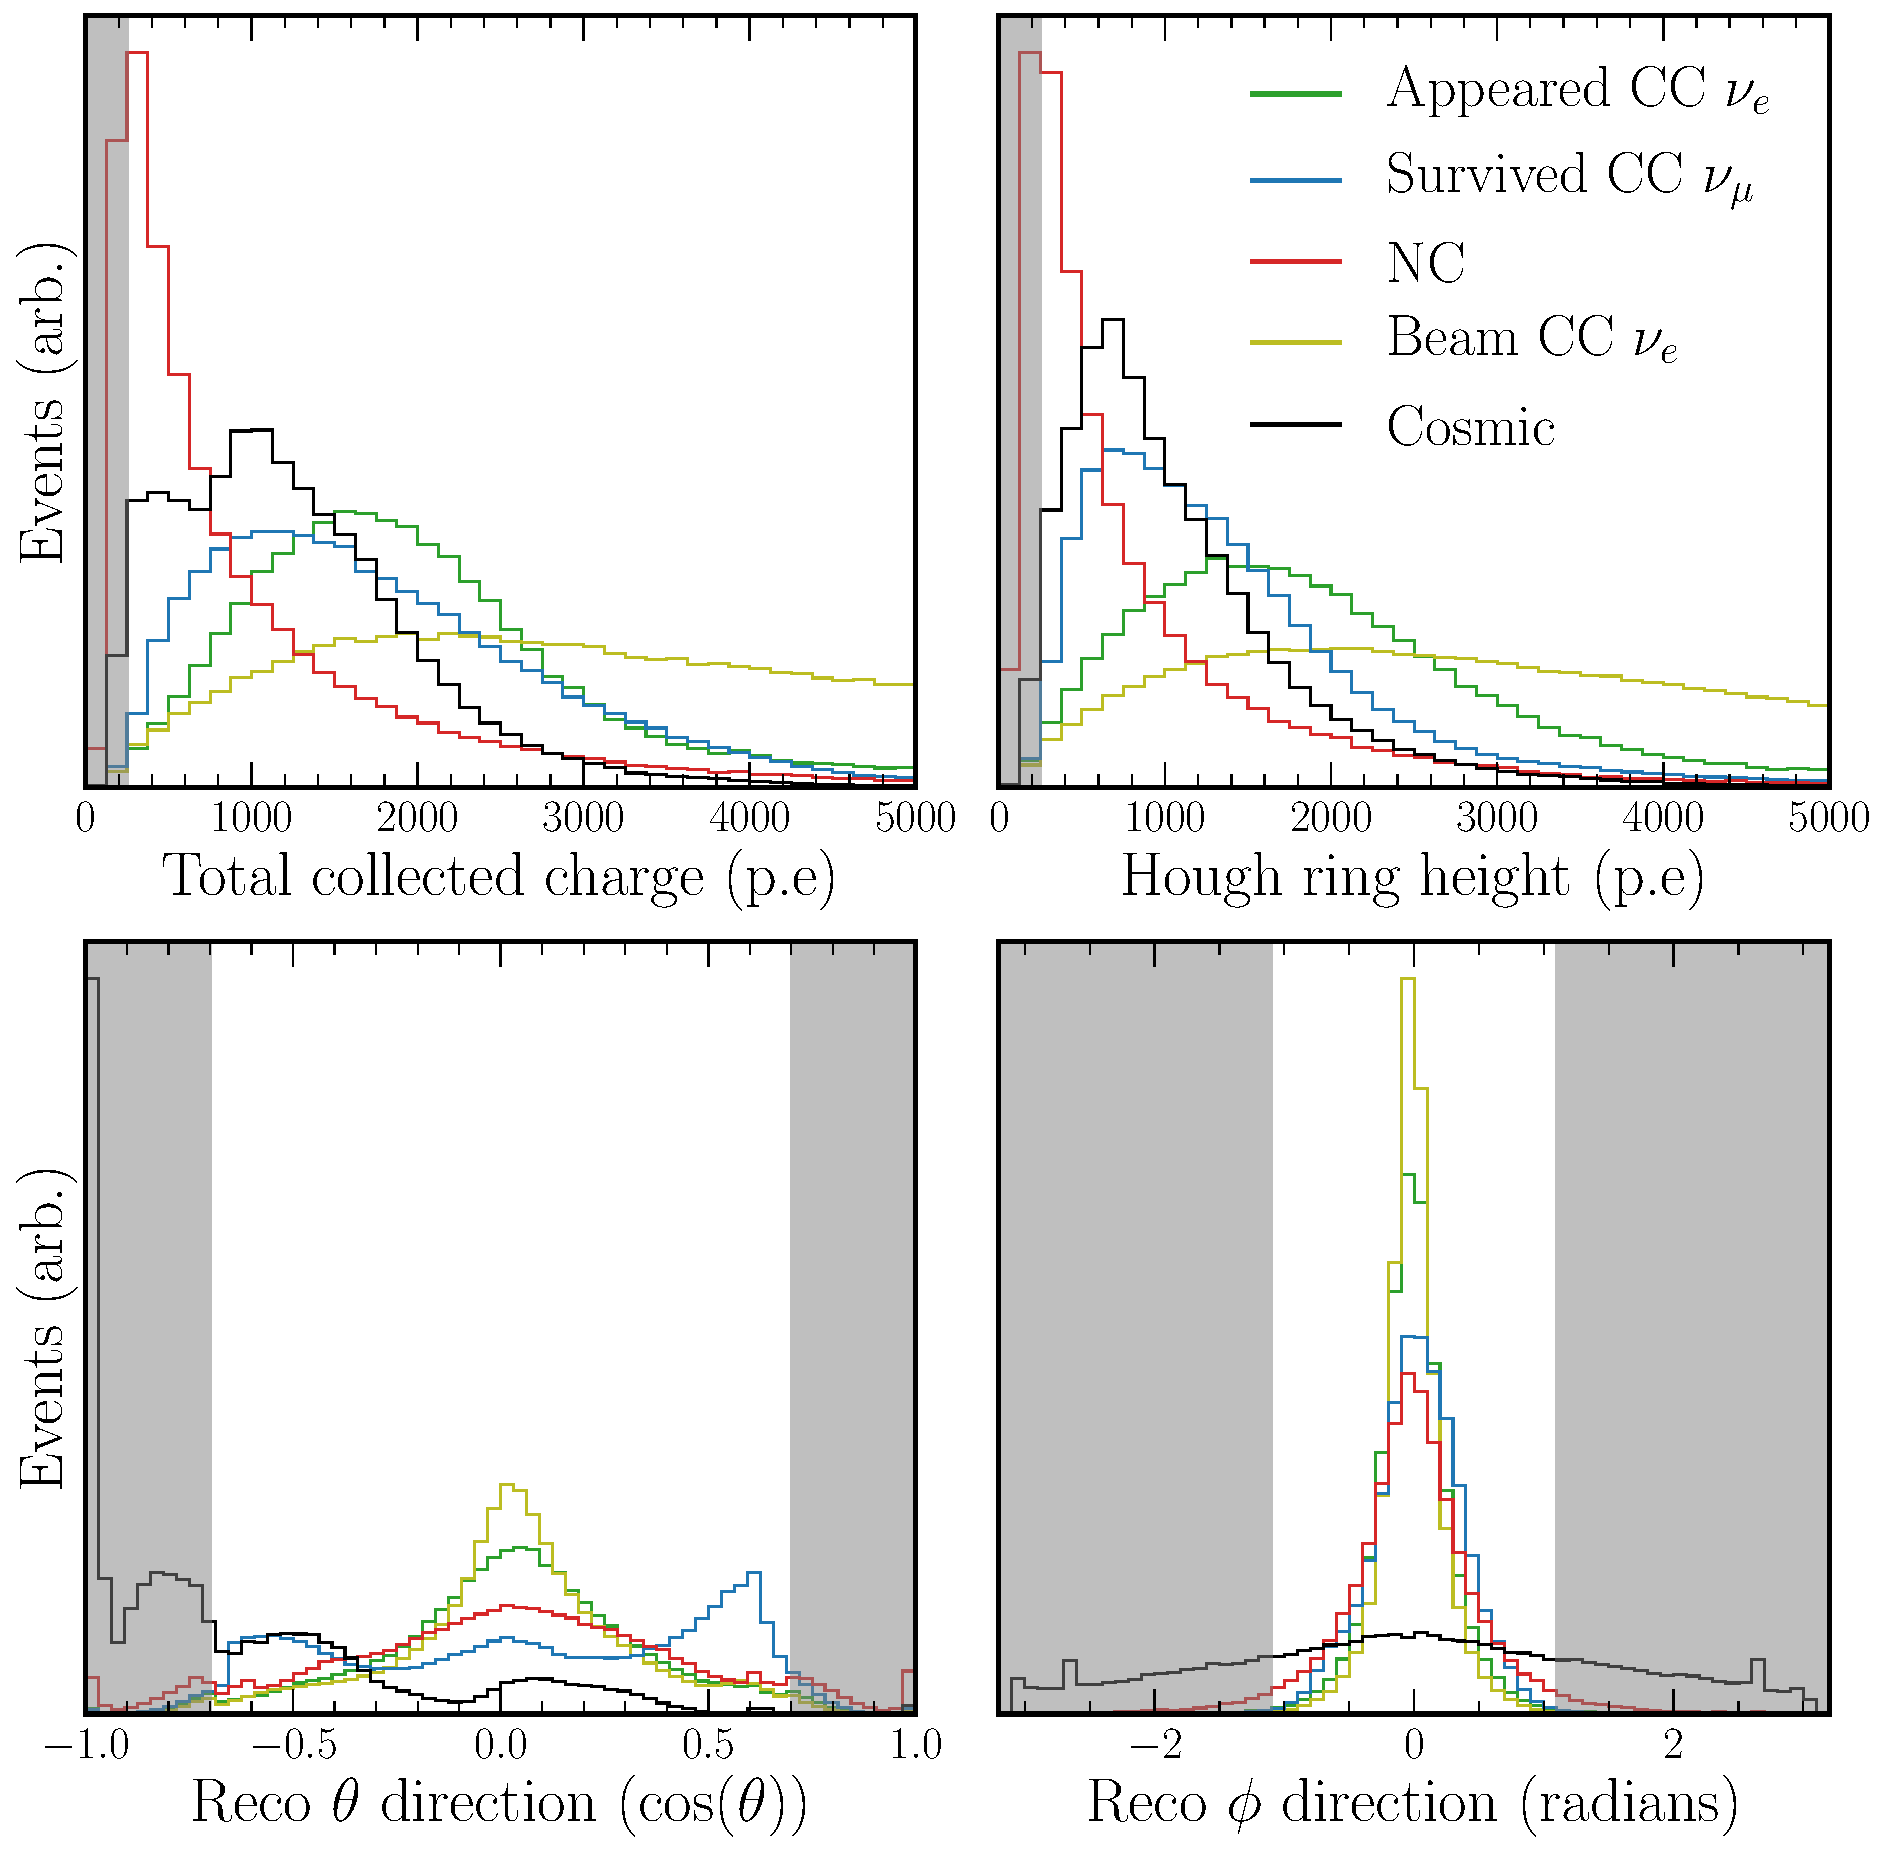
\includegraphics[width=0.8\textwidth]{diagrams/6-cvn/chipsnet/explore_simple_cuts.pdf}
    \caption[explore simple cuts short]
    {explore simple cuts long}
    \label{fig:explore_simple_cuts}
\end{figure}

EXPLAIN WHAT HAS BEEN IMPLEMENTED AS IT WAS FOUND TO BE THE BEST THEN INCLUDE PLOTS AS FOR YOU
INTEREST.
I WILL POINT OUT THE KEY FINDINGS IN OPTIMISATION OF THE NETWORK

PLAN
- Explain the primary task we are trying to solve and how we will judge how well it have done.
Which output scores will we use to compare etc... Although we will use a similar implementation
for both cosmic rejection and energy estimation, primary we are looking for electron neutrino
identification in beam events. Just talk about nuel scores for this first section. We have a
independent test dataset that is scaled to match the events expected in CHIPS. Energy spectrum,
type of neutrino interaction, number of events expected table etc...
- MODEL EVALUATION + TESTING SAMPLE
- SOFTWARE IMPLEMENTATION + TRAINING
- TRAINING SAMPLE
- EVENT REPRESENTATION
- NETWORK ARCHITECTURE
- MULTI-TASK METHODOLOGY

\subsection{Software implementation} %%%%%%%%%%%%%%%%%%%%%%%%%%%%%%%%%%%%%%%%%%%%%%%%%%%%%%%%%%%%%
\label{sec:cvn_baseline_soft} %%%%%%%%%%%%%%%%%%%%%%%%%%%%%%%%%%%%%%%%%%%%%%%%%%%%%%%%%%%%%%%%%%%%

FACTS
- We have developed the `chipsnet' python package built intop of the Tensorflow framework.
- We use Tensorflow framework initially developed by Google
- Makes training across multiple graphics processing units (GPUs) easy to implement.
- We use the Tensorflow dataset API which creates an efficient input pipeline for training data,
allowing it to be loaded on the fly at training time. Impossible to load everything into memory.
- The input files are loaded and random events are loaded into memory decoded and any
manipulations applied before use in training.
- The use of parrallelism allows for all CPU cores (and threads) to be used for loading and
preprocessing data for the GPU batch training process. Preloading the data so it is ready for when
it is needed.
- To optimise data storage and training speed at the training stage all inputs are encoded using
8-bits, with the scaling determined to saturate for each channel ~0.001!!! SHOW PLOT Bottleneck at
training becomes the loading of data on the fly and not the actual network calculations done on
the GPUs.
- Input data is scaled for all channels to be between [0, 1]
- Training data is split into a train and validation dataset 95-5\% split.
- We apply augmentation to the images apply a random factor scaling to each input pixel of
2\% for all channels. Clipping any negative values this produces back to zero.
- The keras high-level API is used within Tensorflow to implement the networks using pre defined
common layers.
- Mini-batch training strategy was used.
- The SHERPA hyperparameter tuning framework was used for hyperparameter tuning.
- We use a learning rate determined from hyperparamter studies to converge well,reducing the
learning rate at each step according to
\begin{equation}
    l_{e}=\frac{l_{0}}{1+c_{d}n_{e}}
\end{equation}
where $c_{d}$ is the coefficient of decay set to be 0.5 and $n_{e}$ is the epoch number
- Implement early stopping
- Input are 64*64 images, how do we represent a cylinder?

- Many high level libraries have now been formed, predominantly led by Tensorflow (from google)
and pyTorch (from facebook) making it easier to quickly code and implemented DNNs.

- Primary goal is to classify the neutrino flavour nuel CC, numu CC or NC
- Secondary goal is to then classify the individual interaction mode (QEL, RES, DIS etc...) these
will have different energy resolutions and systematic uncertainties, so seperation can provide
increased sensitivity.

\subsubsection*{Data preparation}

- normalisation of data
- standardisation etc...

\subsubsection*{Hyperparameter optimisation}

- Refer back to the learning rate as a good example
parameter whose value greatly affects how a network trains. Too large and the minimisation will
continue to step over the minima and too small and the time taken to reach the minima will
increase or the minima may never be found.



\subsection{Software implementation} %%%%%%%%%%%%%%%%%%%%%%%%%%%%%%%%%%%%%%%%%%%%%%%%%%%%%%%%%%%%%
\label{sec:cvn_baseline_soft} %%%%%%%%%%%%%%%%%%%%%%%%%%%%%%%%%%%%%%%%%%%%%%%%%%%%%%%%%%%%%%%%%%%%

- Early stopping
- Model (dropout, batch norm, se, vgg etc...)

[0,25], outside range: 0.0010
    [0,120], outside range: 0.0015
    [0,3500], outside range: 0.0023

\begin{figure} % 8-BIT DIAGRAM %
    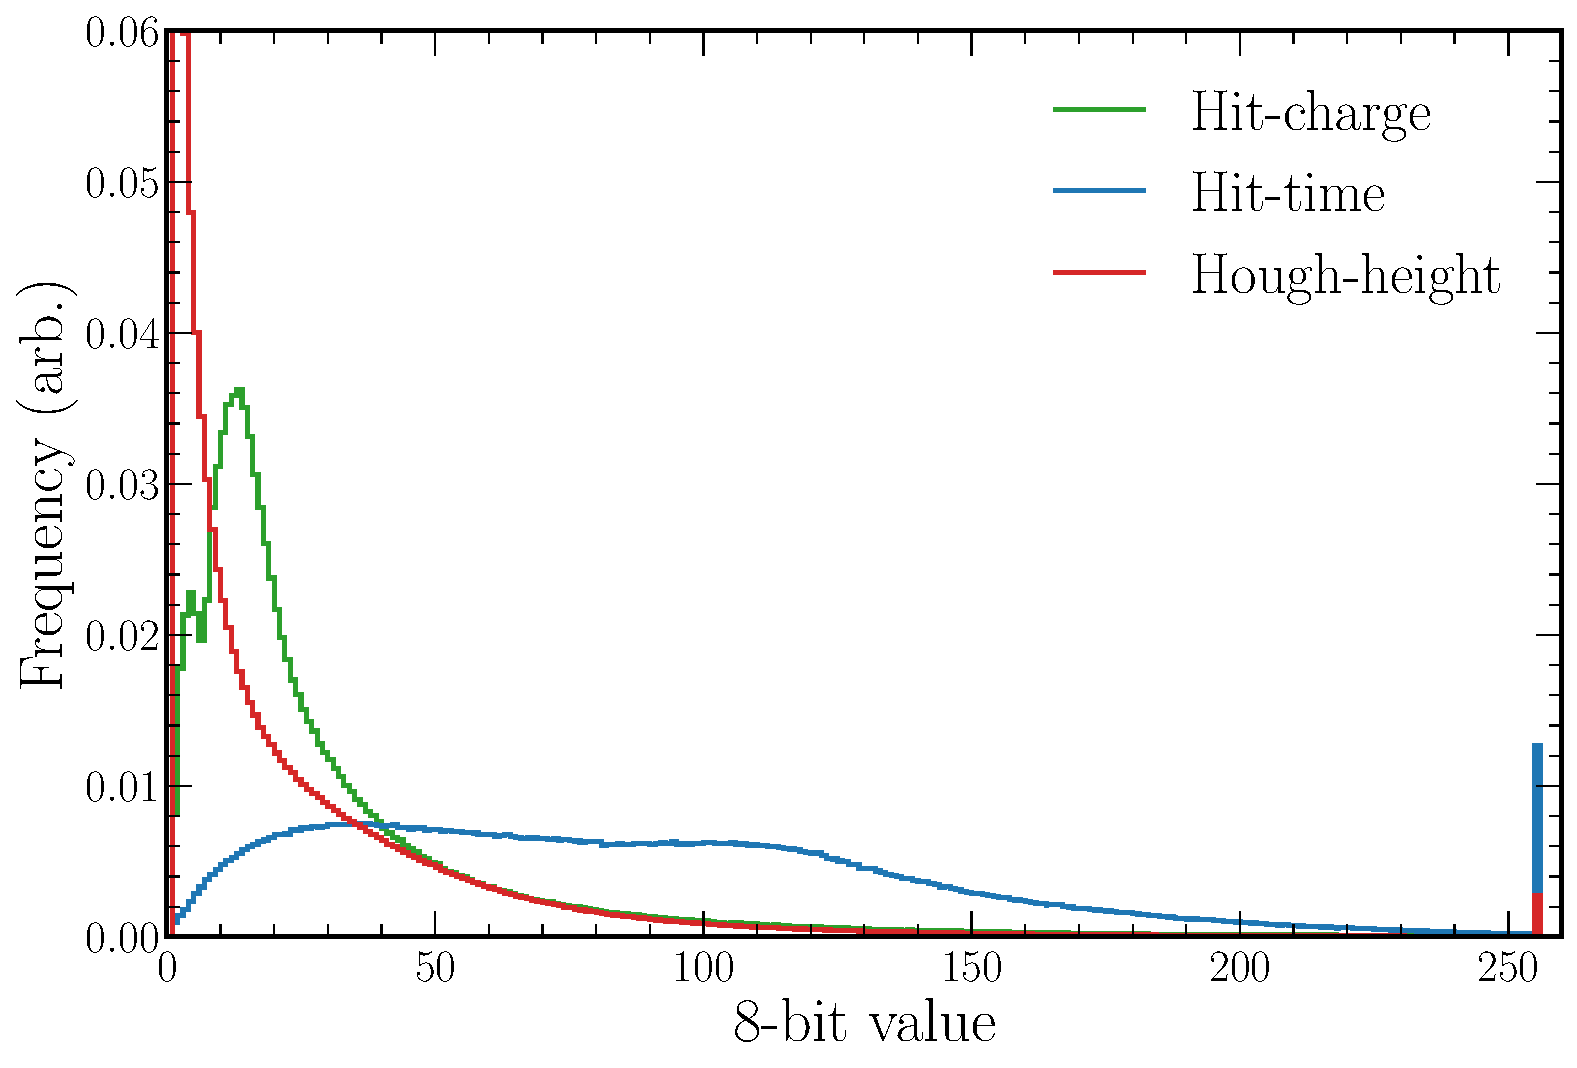
\includegraphics[width=0.6\textwidth]{diagrams/6-cvn/chipsnet/explore_8_bit_range.pdf}
    \caption[explore 8 bit range short]
    {explore 8 bit range long}
    \label{fig:explore_8_bit_range}
\end{figure}

\subsection{Network architecture} %%%%%%%%%%%%%%%%%%%%%%%%%%%%%%%%%%%%%%%%%%%%%%%%%%%%%%%%%%%%%%%%
\label{sec:cvn_baseline_architecture} %%%%%%%%%%%%%%%%%%%%%%%%%%%%%%%%%%%%%%%%%%%%%%%%%%%%%%%%%%%%

- truncated versions of the other networks so they have approximately the same number of parameters
to train for making a good comparison.

Squeeze-and-excitation networks paper in Ref.~\cite{hu2018}
\begin{figure} % SQUEEZE-EXITATION BLOCK DIAGRAM %
    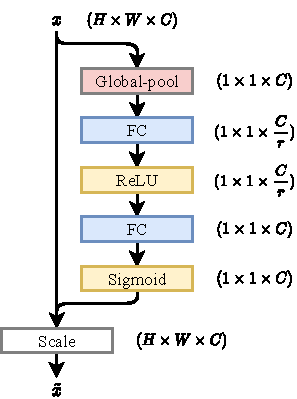
\includegraphics[width=0.4\textwidth]{diagrams/6-cvn/se.pdf}
    \caption[se short]
    {se long}
    \label{fig:se}
\end{figure}

\begin{figure} % CHIPSNET DIAGRAM %
    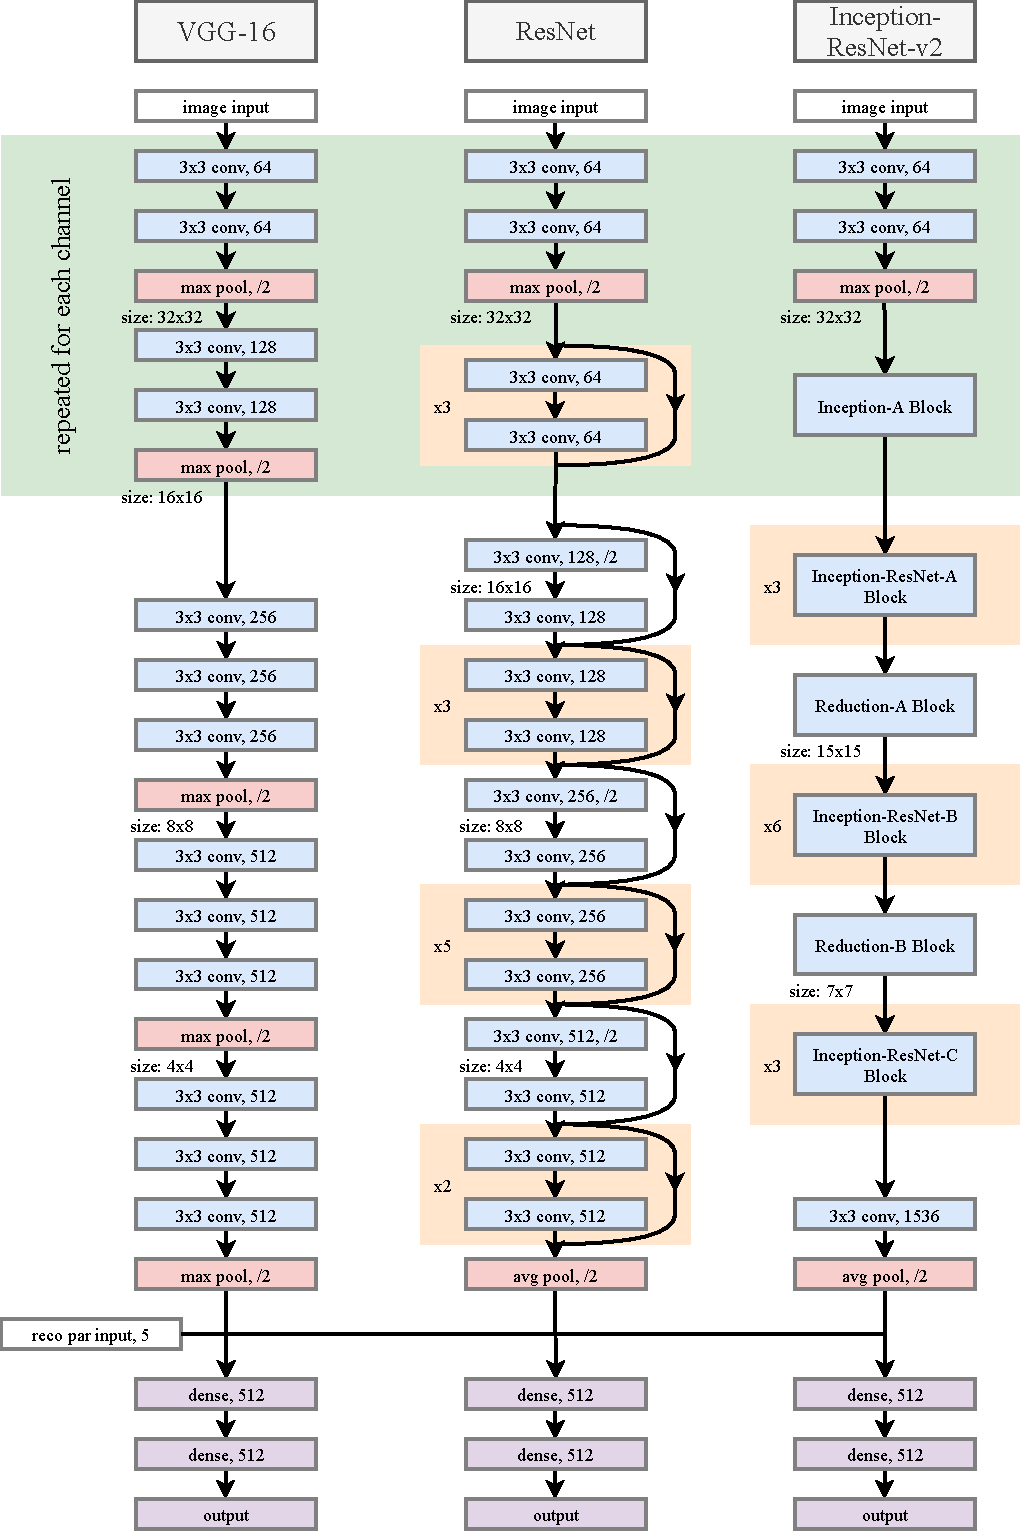
\includegraphics[width=\textwidth]{diagrams/6-cvn/chipsnet.pdf}
    \caption[chipsnet short]
    {chipsnet long}
    \label{fig:chipsnet}
\end{figure}

vgg: 17,225,296 (88ms)
inception: 16,893,216 (192ms)
resnet: 16,526,288 (112ms)
inception-resnet: 17,145,238 (209ms)

\begin{figure} % ARCHITECTURE NUEL EFF CURVES DIAGRAM %
    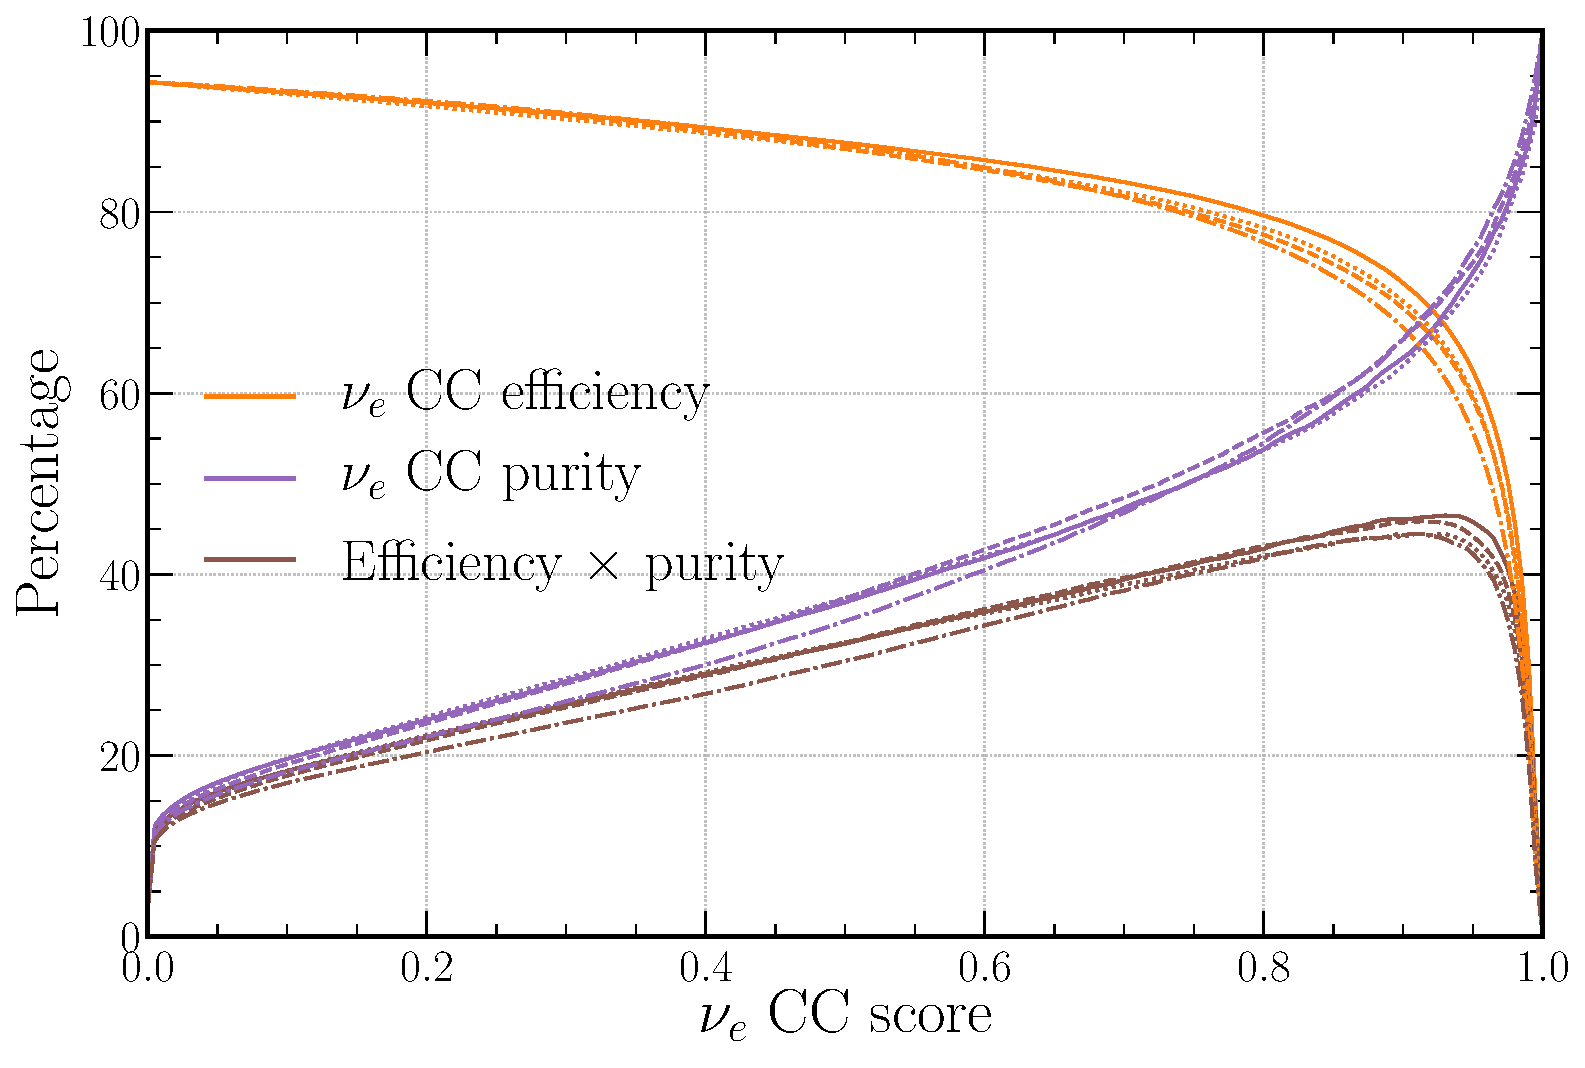
\includegraphics[width=0.6\textwidth]{diagrams/6-cvn/chipsnet/arch_nuel_eff_curves.pdf}
    \caption[arch nuel eff curves short]
    {vgg=solid, inception=dashed, resnet=dotted, inception-resnet=dot-dash}
    \label{fig:arch_nuel_eff_curves}
\end{figure}

\begin{figure} % ARCHITECTURE NUEL COMP CURVES DIAGRAM %
    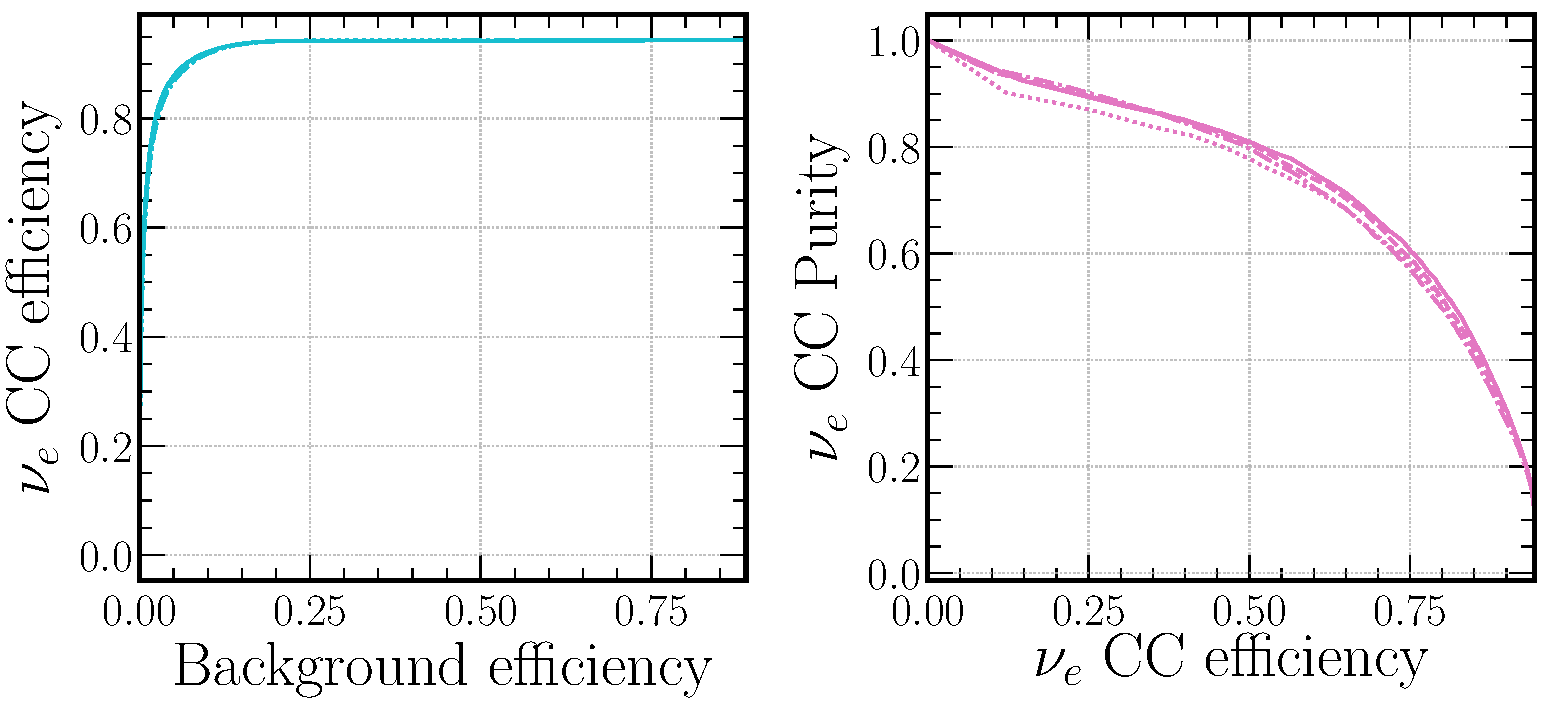
\includegraphics[width=0.8\textwidth]{diagrams/6-cvn/chipsnet/arch_nuel_comp_curves.pdf}
    \caption[arch nuel comp curves short]
    {vgg=solid, inception=dashed, resnet=dotted, inception-resnet=dot-dash}
    \label{fig:arch_nuel_comp_curves}
\end{figure}

- Nuel-> ROC-AUC: 0.82559, PRC-AUC: 0.71155, S-Eff: 0.87661, S-Pur: 0.36928
- FOM1-> 0.46510, 0.93000, 53.44422, 8.34671, 15.75487, 0.67485, 0.68920
- FOM2-> 13.44645, 0.98500, 31.21664, 1.57028, 3.81933, 0.39418, 0.85277

- Nuel-> ROC-AUC: 0.82519, PRC-AUC: 0.70632, S-Eff: 0.86992, S-Pur: 0.37332
- FOM1-> 0.45910, 0.91500, 53.20954, 9.73154, 14.92970, 0.67188, 0.68331
- FOM2-> 13.47965, 0.98500, 28.04995, 1.43802, 2.89217, 0.35419, 0.86627

- Nuel-> ROC-AUC: 0.82444, PRC-AUC: 0.68789, S-Eff: 0.86926, S-Pur: 0.37417
- FOM1-> 0.44511, 0.91000, 54.46409, 11.50537, 18.18029, 0.68772, 0.64723
- FOM2-> 12.22026, 0.98000, 32.56108, 2.77151, 4.32813, 0.41115, 0.82099

- Nuel-> ROC-AUC: 0.82444, PRC-AUC: 0.69946, S-Eff: 0.87369, S-Pur: 0.34882
- FOM1-> 0.44448, 0.90500, 52.61119, 10.90981, 15.11323, 0.66433, 0.66906
- FOM2-> 13.48962, 0.98500, 23.98040, 0.96809, 2.19211, 0.30280, 0.88356

\subsection{Which training sample to use} %%%%%%%%%%%%%%%%%%%%%%%%%%%%%%%%%%%%%%%%%%%%%%%%%%%%%%%%
\label{sec:cvn_baseline_sample} %%%%%%%%%%%%%%%%%%%%%%%%%%%%%%%%%%%%%%%%%%%%%%%%%%%%%%%%%%%%%%%%%%

- See signal interactions peaked closely near score values of unity and the backgrounds lie close
to the zero score as expected.

\begin{figure} % FLUX TRAINING SAMPLE DIAGRAM %
    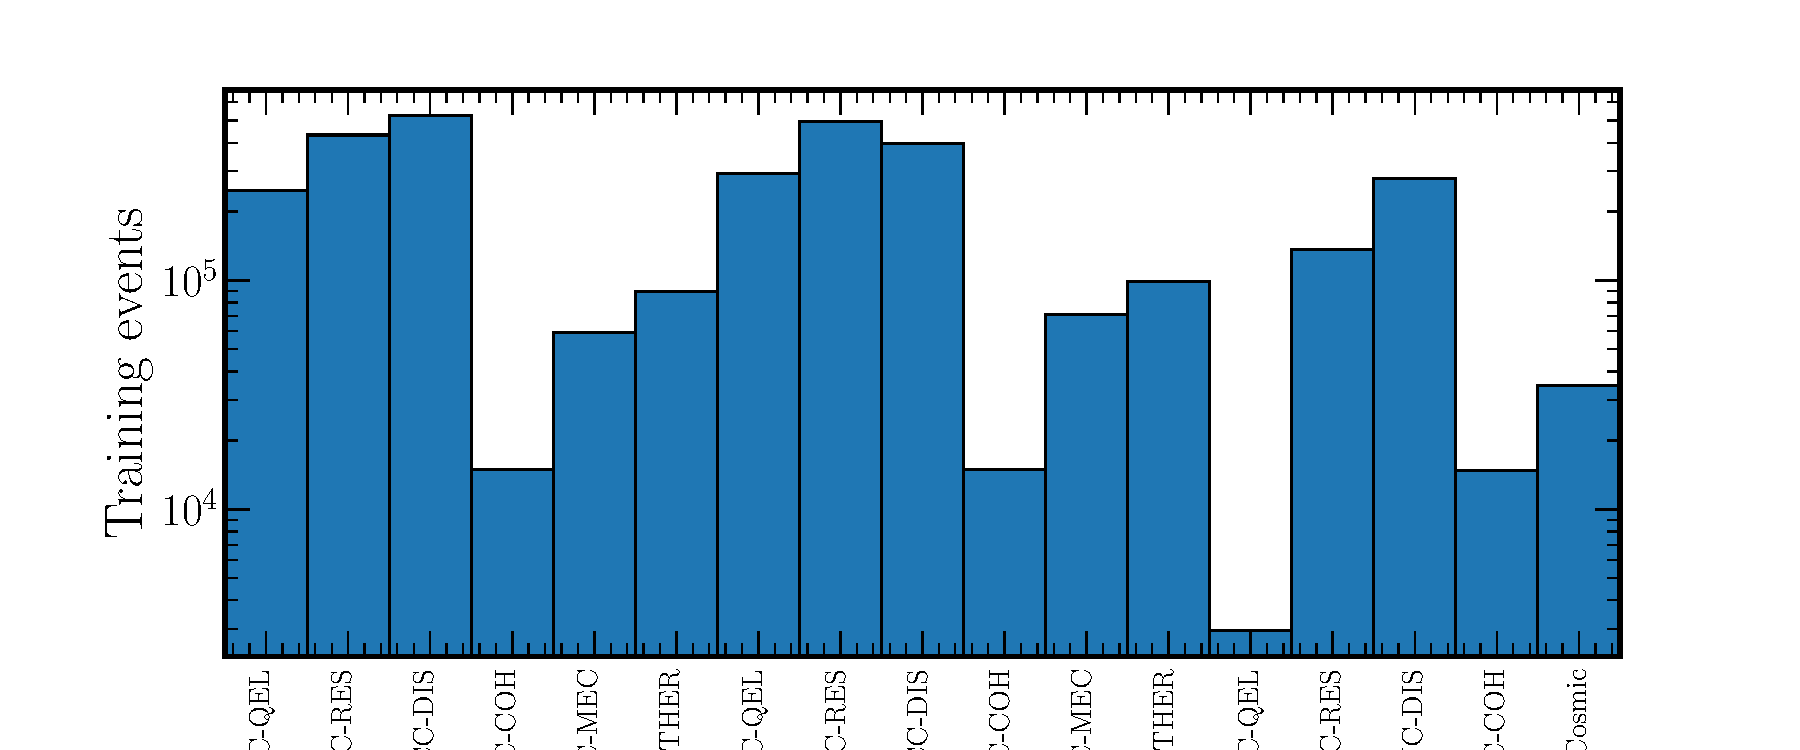
\includegraphics[width=0.6\textwidth]{diagrams/6-cvn/chipsnet/explore_flux_sample.pdf}
    \caption[explore flux sample short]
    {explore flux sample long}
    \label{fig:explore_flux_sample}
\end{figure}

\begin{figure} % UNIFORM TRAINING SAMPLE DIAGRAM %
    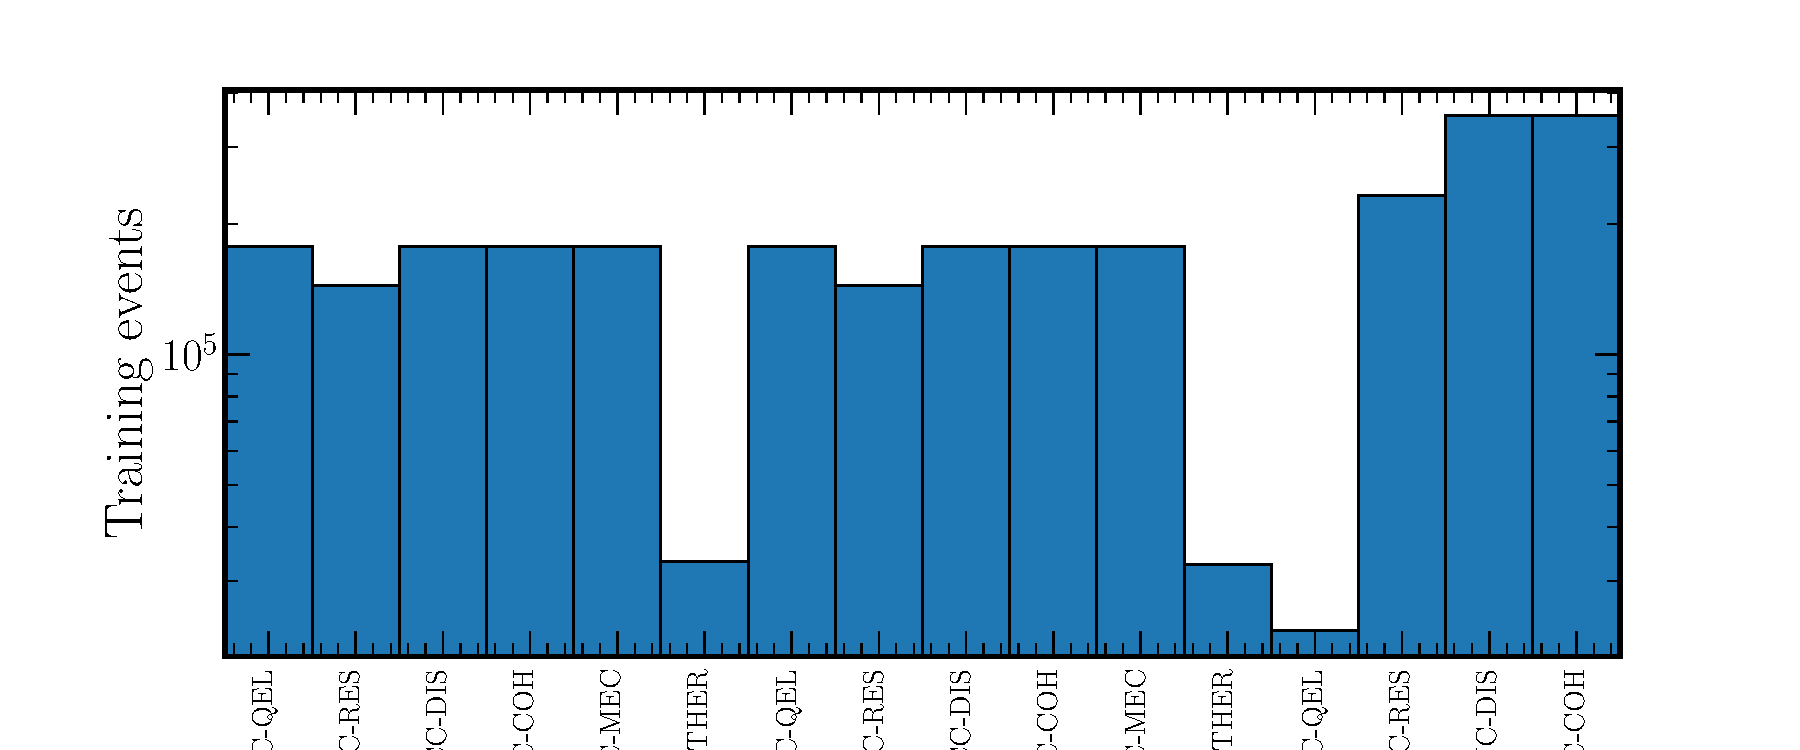
\includegraphics[width=0.6\textwidth]{diagrams/6-cvn/chipsnet/explore_uniform_sample.pdf}
    \caption[explore uniform sample short]
    {explore uniform sample long}
    \label{fig:explore_uniform_sample}
\end{figure}

\begin{figure} % BOTH TRAINING SAMPLE DIAGRAM %
    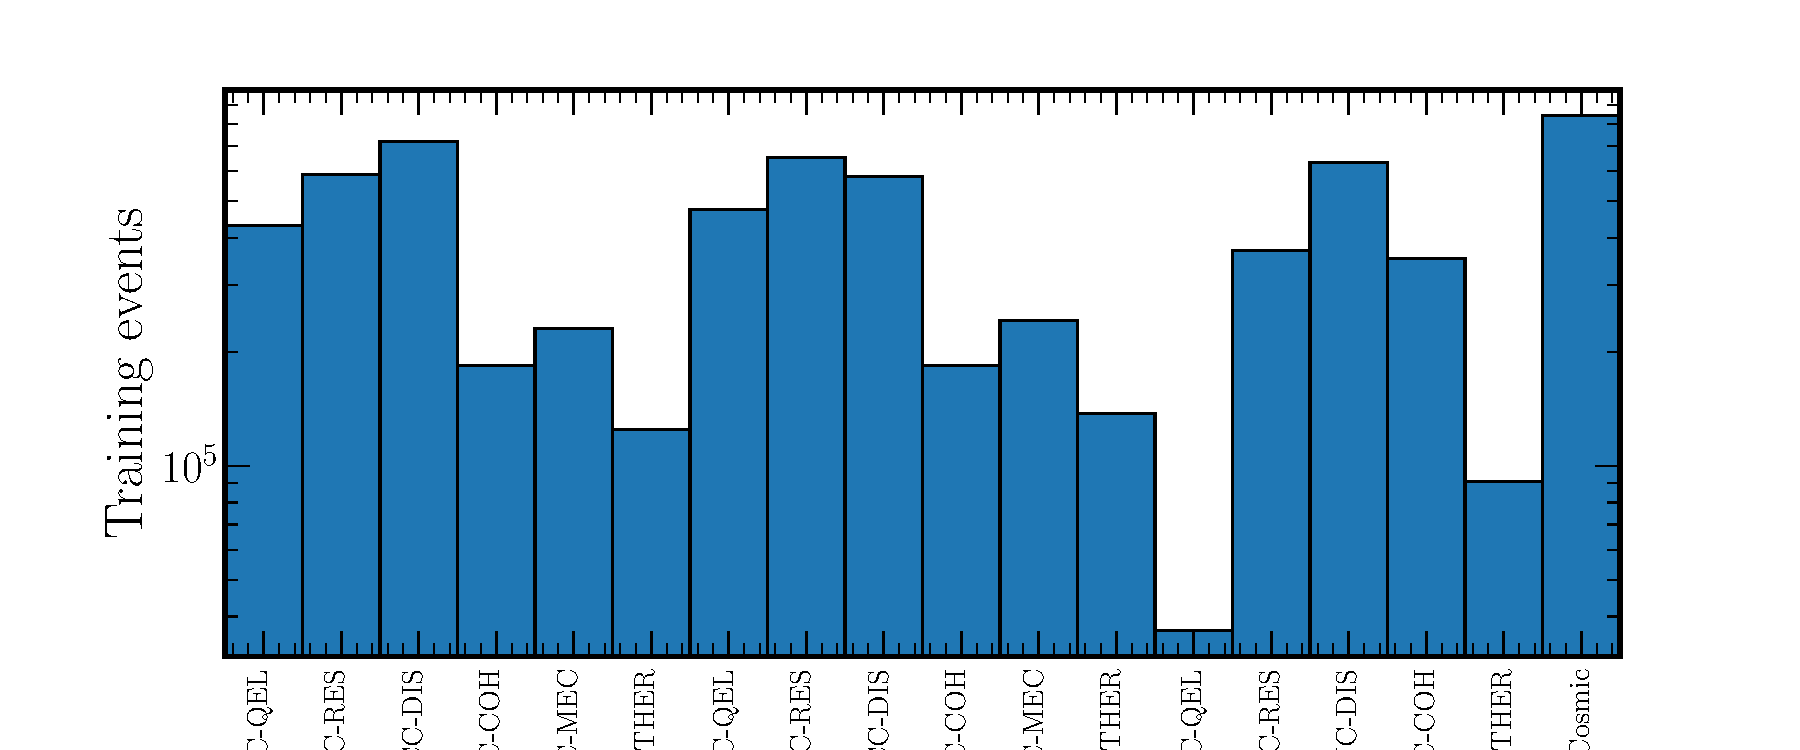
\includegraphics[width=0.6\textwidth]{diagrams/6-cvn/chipsnet/explore_both_sample.pdf}
    \caption[explore both sample short]
    {explore both sample long}
    \label{fig:explore_both_sample}
\end{figure}

\begin{figure} % SAMPLE FLUX OUTPUT DIAGRAM %
    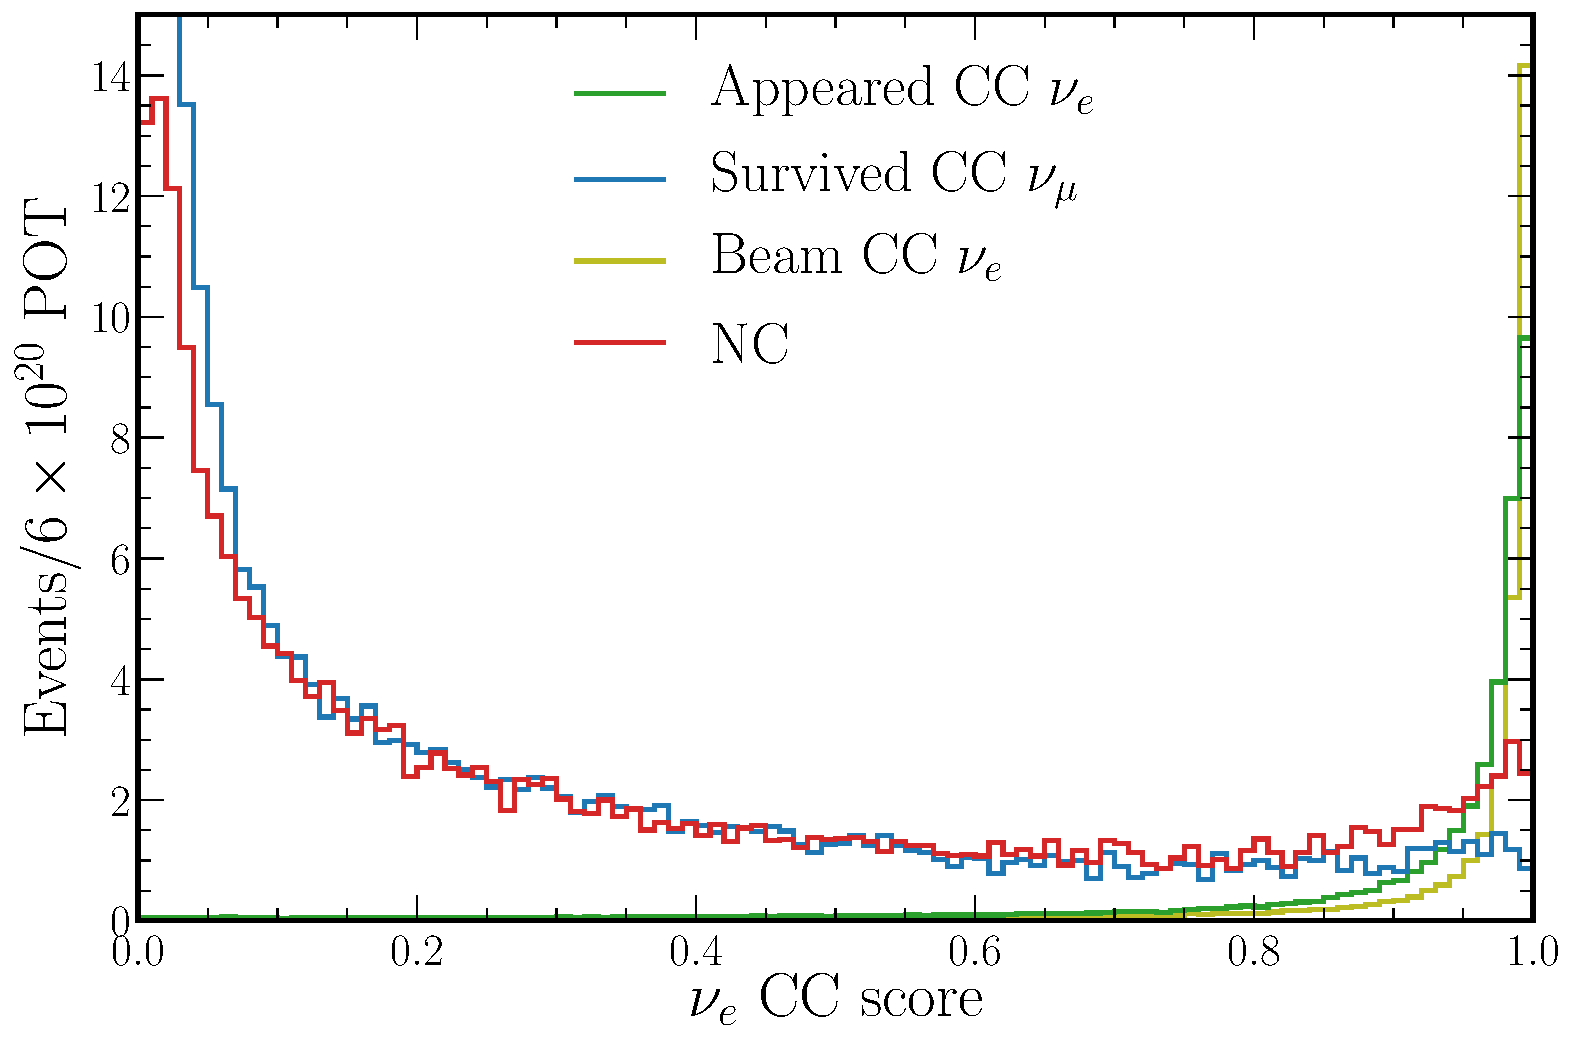
\includegraphics[width=0.6\textwidth]{diagrams/6-cvn/chipsnet/sample_flux_output_values.pdf}
    \caption[sample flux output values short]
    {sample flux output values long}
    \label{fig:sample_flux_output_values}
\end{figure}

\begin{figure} % SAMPLE UNIFORM OUTPUT DIAGRAM %
    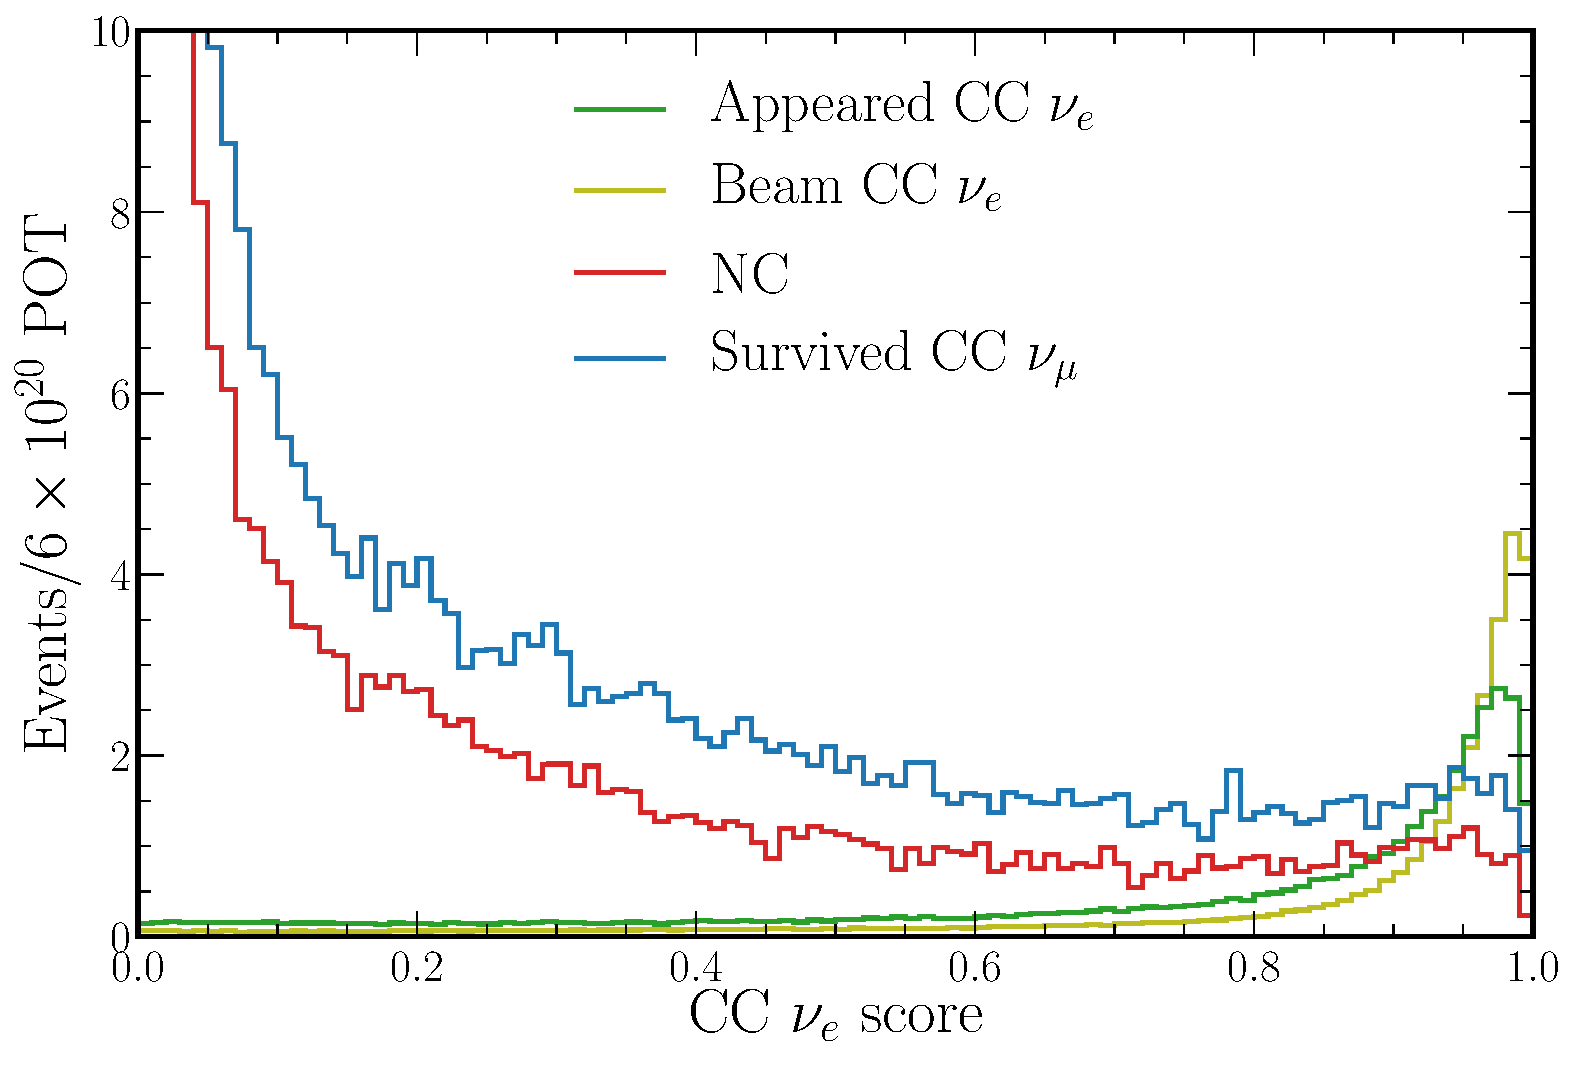
\includegraphics[width=0.6\textwidth]{diagrams/6-cvn/chipsnet/sample_uniform_output_values.pdf}
    \caption[sample uniform output values short]
    {sample uniform output values long}
    \label{fig:sample_uniform_output_values}
\end{figure}

\begin{figure} % SAMPLE BOTH OUTPUT DIAGRAM %
    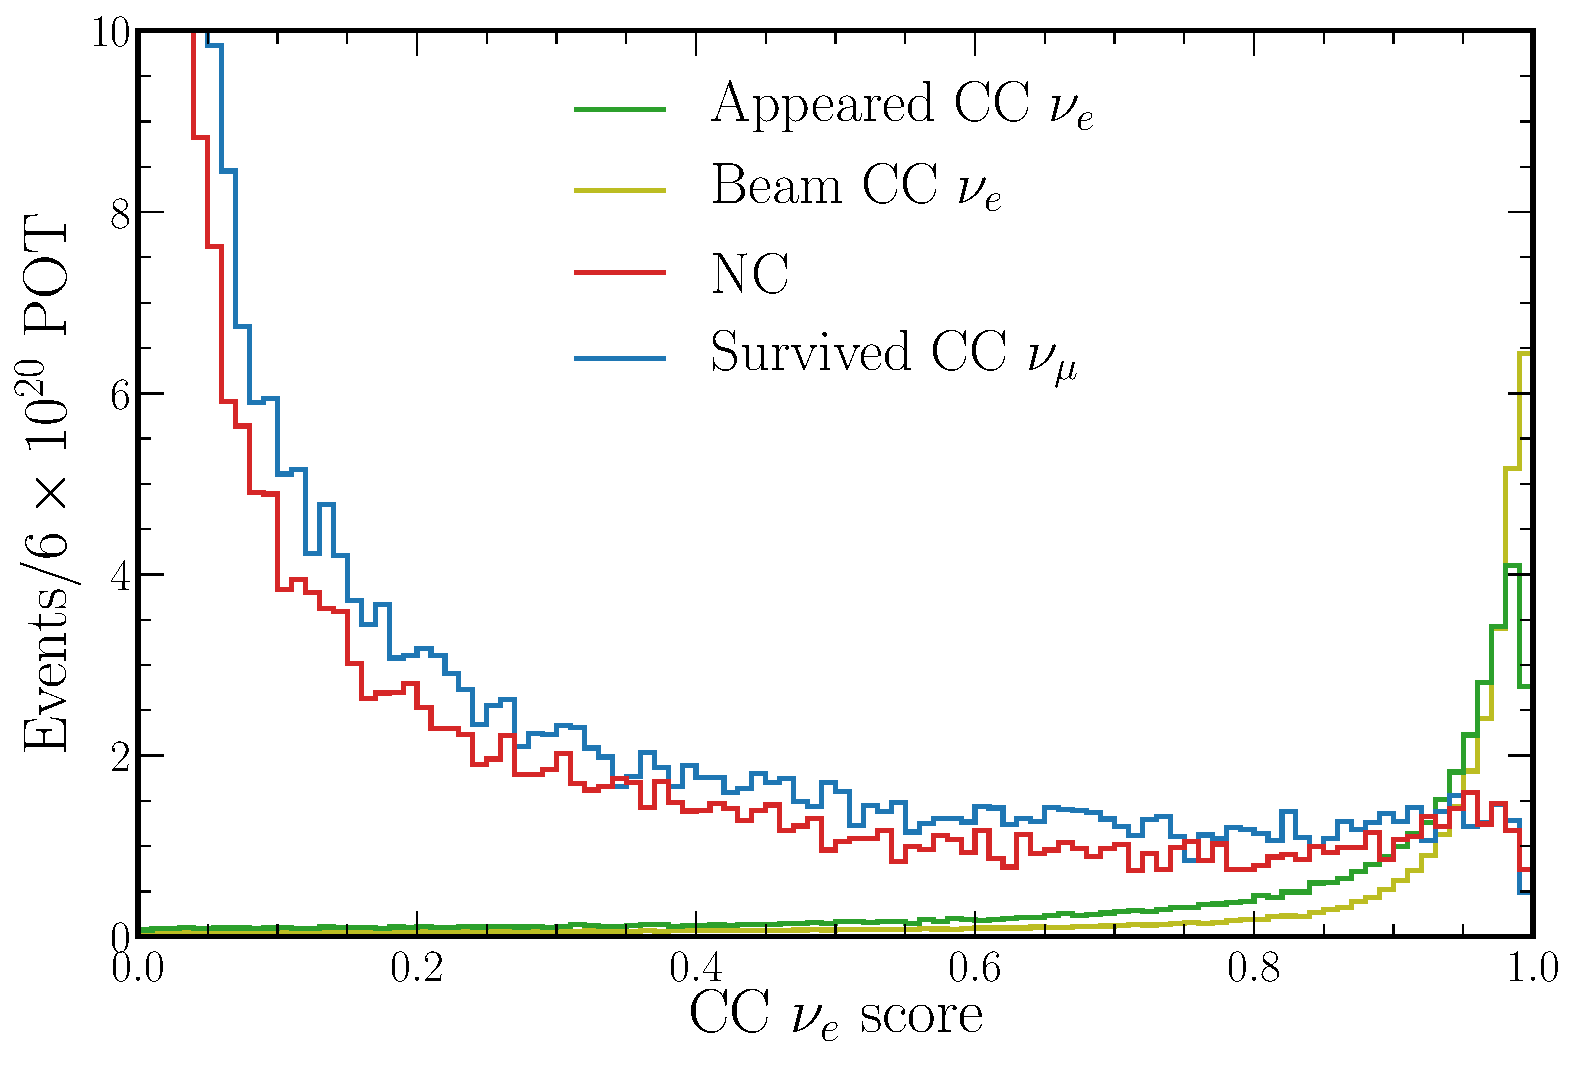
\includegraphics[width=0.6\textwidth]{diagrams/6-cvn/chipsnet/sample_both_output_values.pdf}
    \caption[sample both output values short]
    {sample both output values long}
    \label{fig:sample_both_output_values}
\end{figure}

\begin{figure} % SAMPLE NUEL EFF CURVES DIAGRAM %
    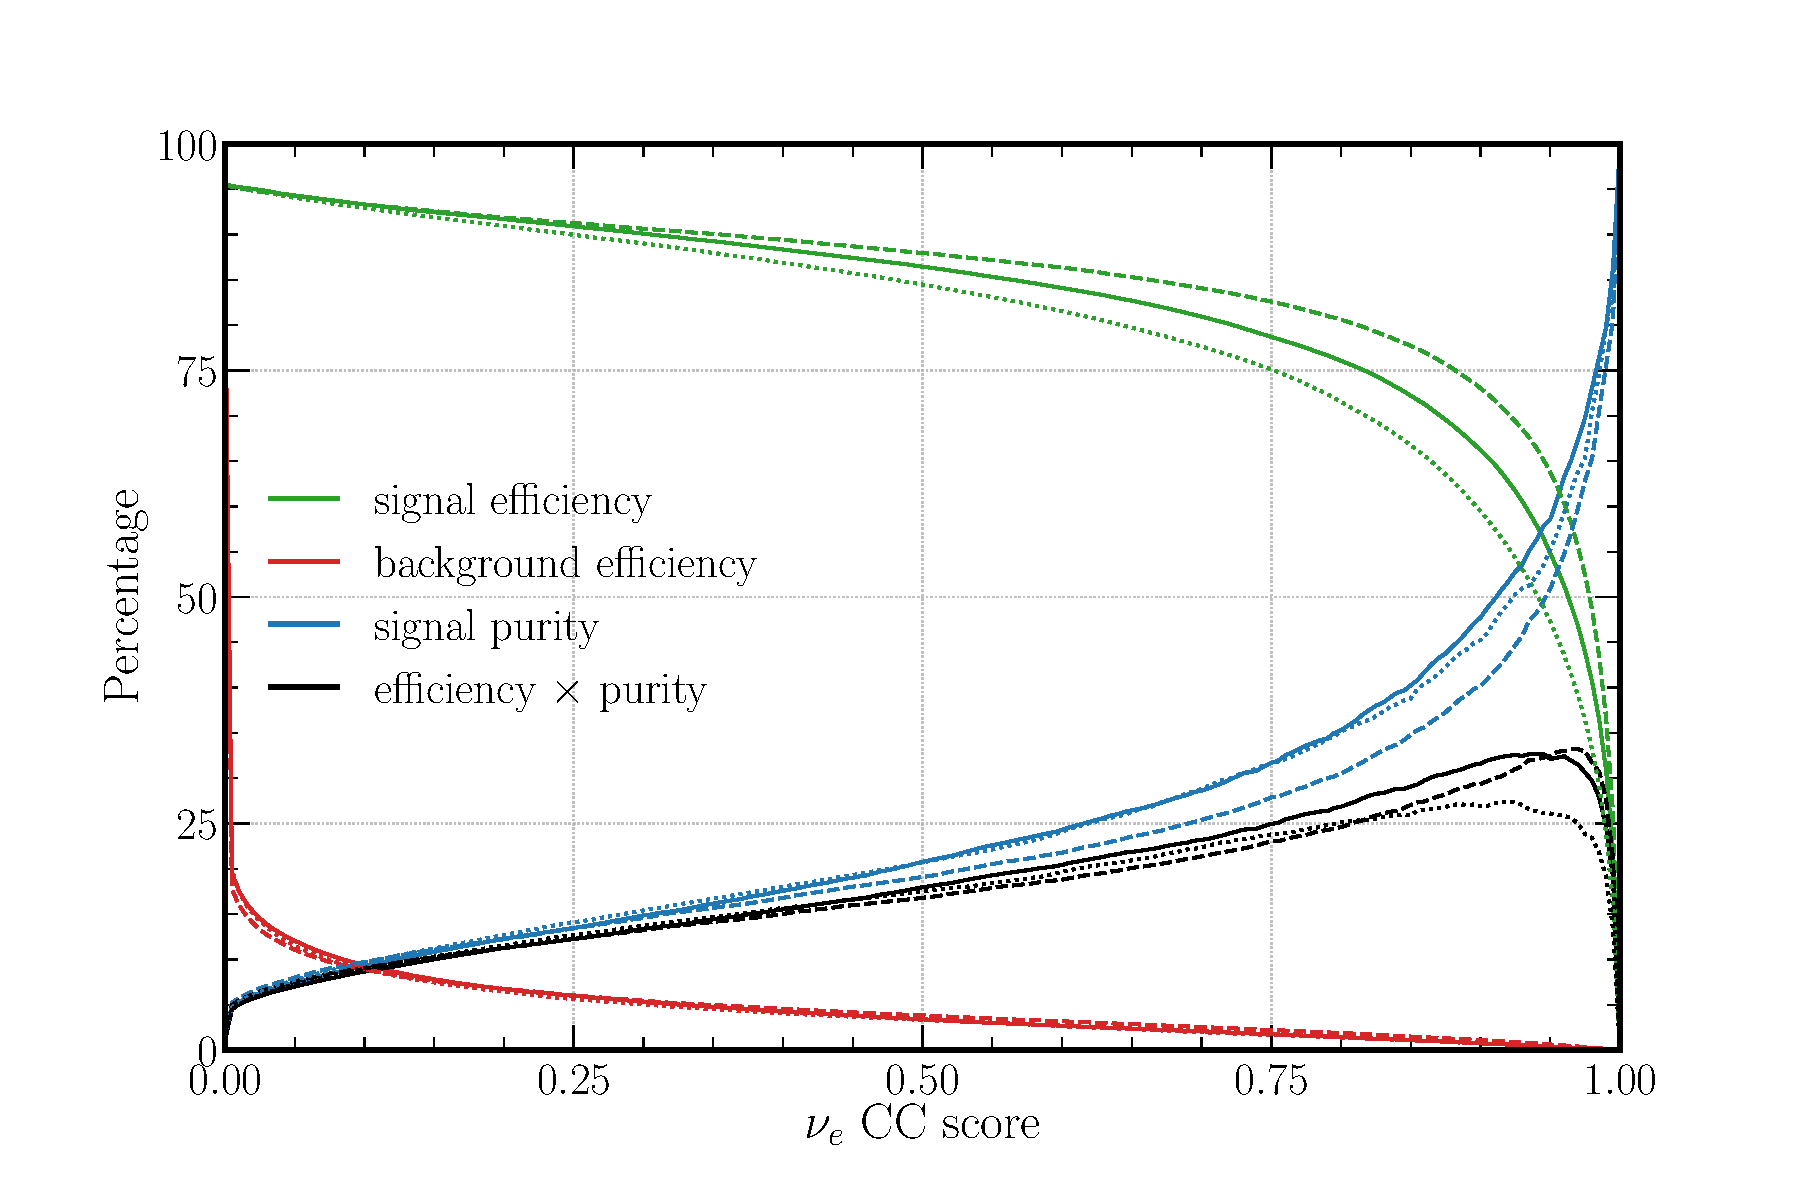
\includegraphics[width=0.6\textwidth]{diagrams/6-cvn/chipsnet/sample_nuel_eff_curves.pdf}
    \caption[sample nuel eff curves short]
    {both=solid, flux=dashed, uniform=dotted}
    \label{fig:sample_nuel_eff_curves}
\end{figure}

\begin{figure} % SAMPLE NUEL COMP CURVES DIAGRAM %
    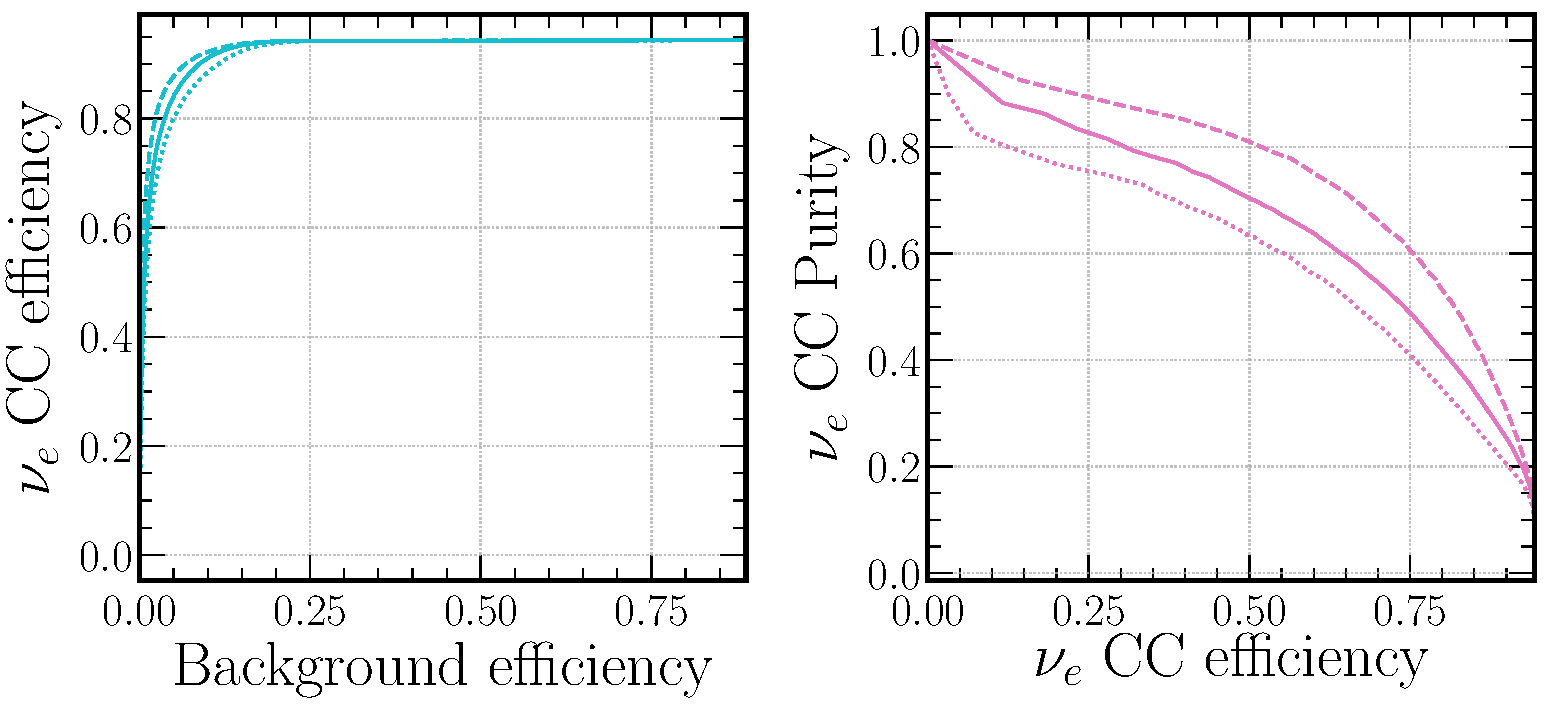
\includegraphics[width=0.8\textwidth]{diagrams/6-cvn/chipsnet/sample_nuel_comp_curves.pdf}
    \caption[sample nuel comp curves short]
    {both=solid, flux=dashed, uniform=dotted}
    \label{fig:sample_nuel_comp_curves}
\end{figure}

- Nuel-> ROC-AUC: 0.82559, PRC-AUC: 0.71155, S-Eff: 0.87661, S-Pur: 0.36928
- FOM1-> 0.46510, 0.93000, 53.44422, 8.34671, 15.75487, 0.67485, 0.68920
- FOM2-> 13.44645, 0.98500, 31.21664, 1.57028, 3.81933, 0.39418, 0.85277

- Nuel-> ROC-AUC: 0.81488, PRC-AUC: 0.56769, S-Eff: 0.79933, S-Pur: 0.34677
- FOM1-> 0.33905, 0.82500, 49.50120, 26.12079, 15.63656, 0.62506, 0.54243
- FOM2-> 8.44226, 0.92500, 36.01710, 11.59853, 6.60268, 0.45479, 0.66430

- Nuel-> ROC-AUC: 0.82063, PRC-AUC: 0.63426, S-Eff: 0.83421, S-Pur: 0.36814
- FOM1-> 0.38628, 0.84000, 52.60971, 19.59654, 18.26900, 0.66431, 0.58148
- FOM2-> 10.10769, 0.96000, 30.52599, 4.49055, 4.63030, 0.38545, 0.76995

\subsection{Which event representation to use} %%%%%%%%%%%%%%%%%%%%%%%%%%%%%%%%%%%%%%%%%%%%%%%%%%%
\label{sec:cvn_baseline_repr} %%%%%%%%%%%%%%%%%%%%%%%%%%%%%%%%%%%%%%%%%%%%%%%%%%%%%%%%%%%%%%%%%%%%

- Cern summer report in Ref.~\cite{theodore2016}
- New ideas with x+ x- mapping in Ref.~\cite{berns2020}
- Fraction of deposited charge in endcaps = 0.4769380479133997


\begin{equation} % ONE-HOT EQUATION %
    X_{\pm}=
    \begin{cases}
        1-\chi_{\mp} & (z \geq 0) \\
        \chi_{\pm}   & (z < 0)
    \end{cases}
\end{equation}

\begin{equation} % ONE-HOT EQUATION %
    \chi_{\pm}=W(\rho,z)\frac{\pi\pm\phi}{2\pi}
\end{equation}

\begin{equation}
    W(\rho,z)=\sqrt{\frac{\rho^{2}-2R\abs{z}+RH}{R^{2}+RH}}
\end{equation}

where R and Z are the radius and height of the detector cylinder and W is chosen for constant
surface density.

- Turns out removing the distortions of not viewing the event from the vertex is the most important
thing!!!


- Approaches in the past for event classification using CNNs for water cherenkov detectors have
taken a few Approaches to generating the input image representation.
- Projecting onto a 2d surface "outside" the detector

\begin{figure} % NUEL EVENT DIAGRAM %
    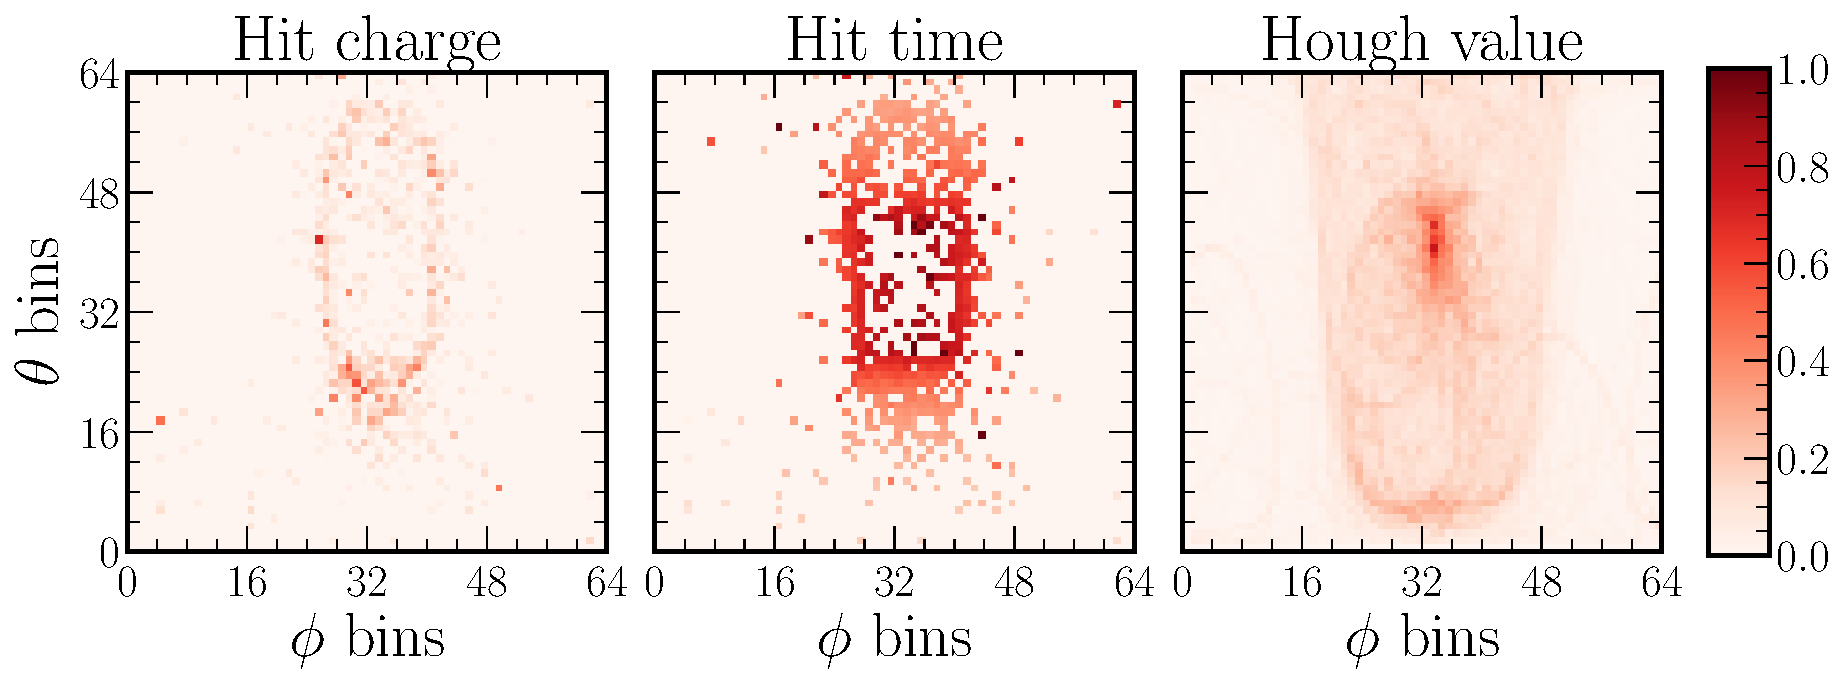
\includegraphics[width=0.8\textwidth]{diagrams/6-cvn/chipsnet/explore_nuel_ccres_event.pdf}
    \caption[explore nuel ccres event short]
    {3
        3307.41
        2777.48
            [  11 2212 2212  111 -999 -999 -999 -999 -999 -999 -999 -999 -999 -999
                -999 -999 -999 -999 -999 -999]
            [2777.48  1085.32   991.703  318.527 -999.    -999.    -999.    -999.
                -999.    -999.    -999.    -999.    -999.    -999.    -999.    -999.
                -999.    -999.    -999.    -999.   ]
        0}
    \label{fig:explore_nuel_ccres_event}
\end{figure}

\begin{figure} % NUMU EVENT DIAGRAM %
    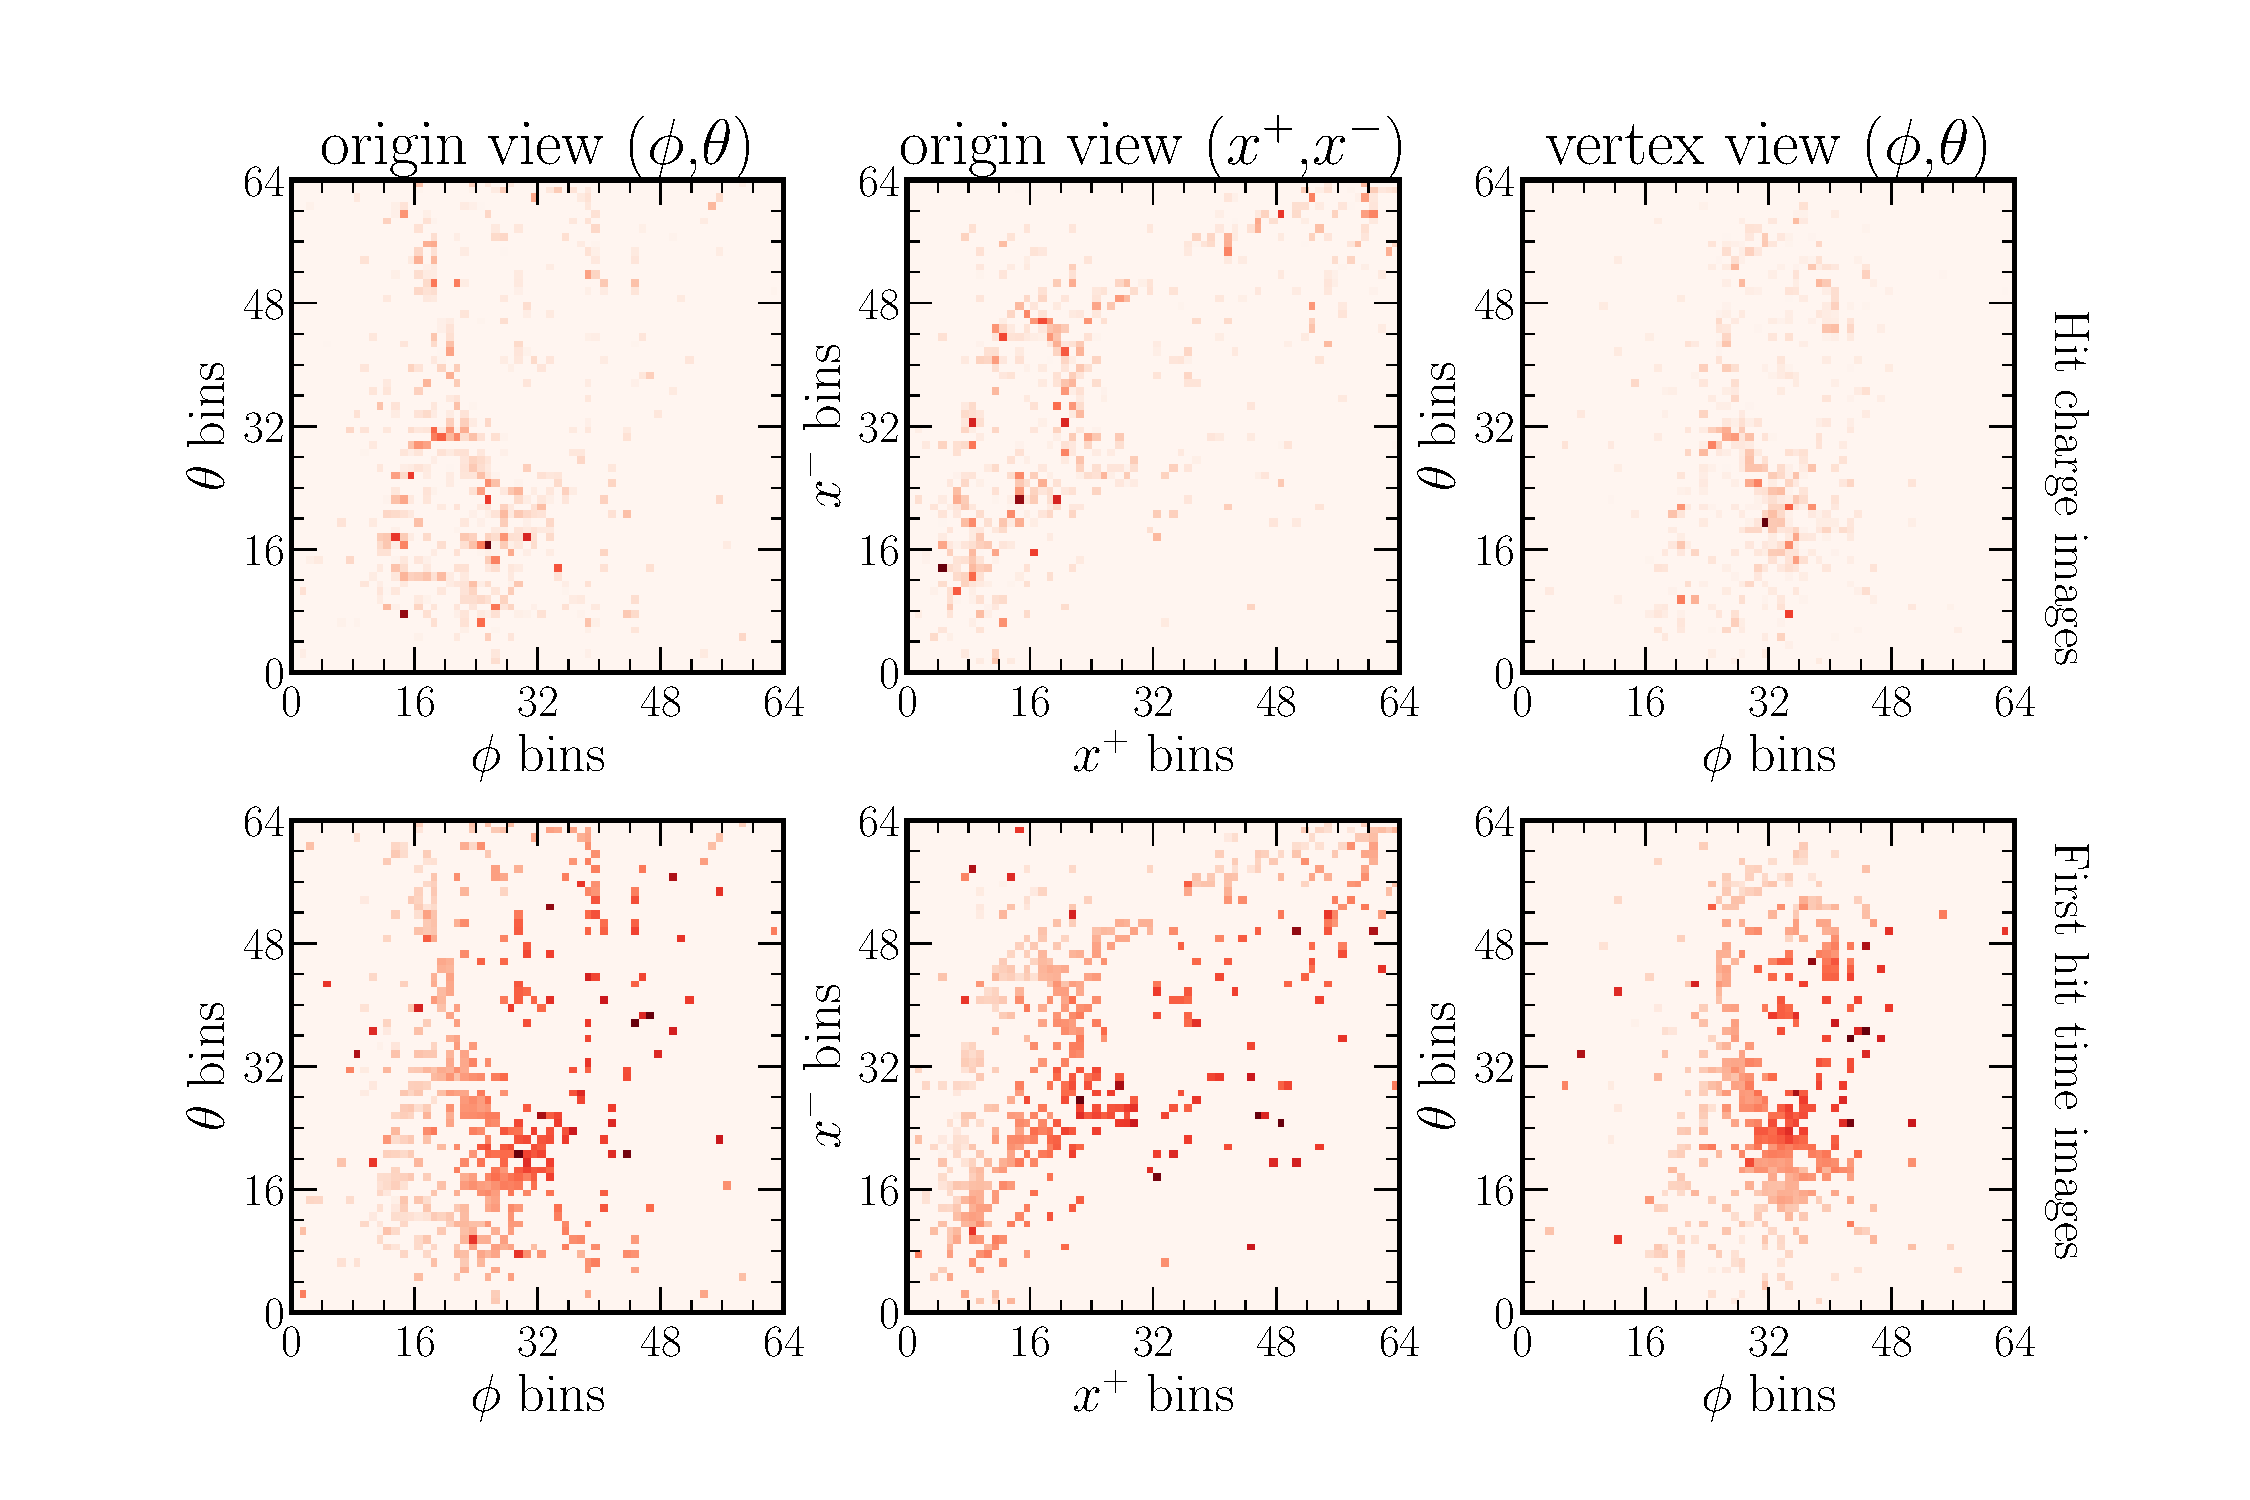
\includegraphics[width=0.8\textwidth]{diagrams/6-cvn/chipsnet/explore_numu_ccdis_event.pdf}
    \caption[explore numu ccdis event short]
    {91
        3520.17
        1862.55
            [2212   13 2112  211  211   22 -999 -999 -999 -999 -999 -999 -999 -999
                -999 -999 -999 -999 -999 -999]
            [2022.37  1862.55  1038.34   226.973  223.71     6.32  -999.    -999.
                -999.    -999.    -999.    -999.    -999.    -999.    -999.    -999.
                -999.    -999.    -999.    -999.   ]
        0}
    \label{fig:explore_numu_ccdis_event}
\end{figure}

\begin{figure} % NC EVENT DIAGRAM %
    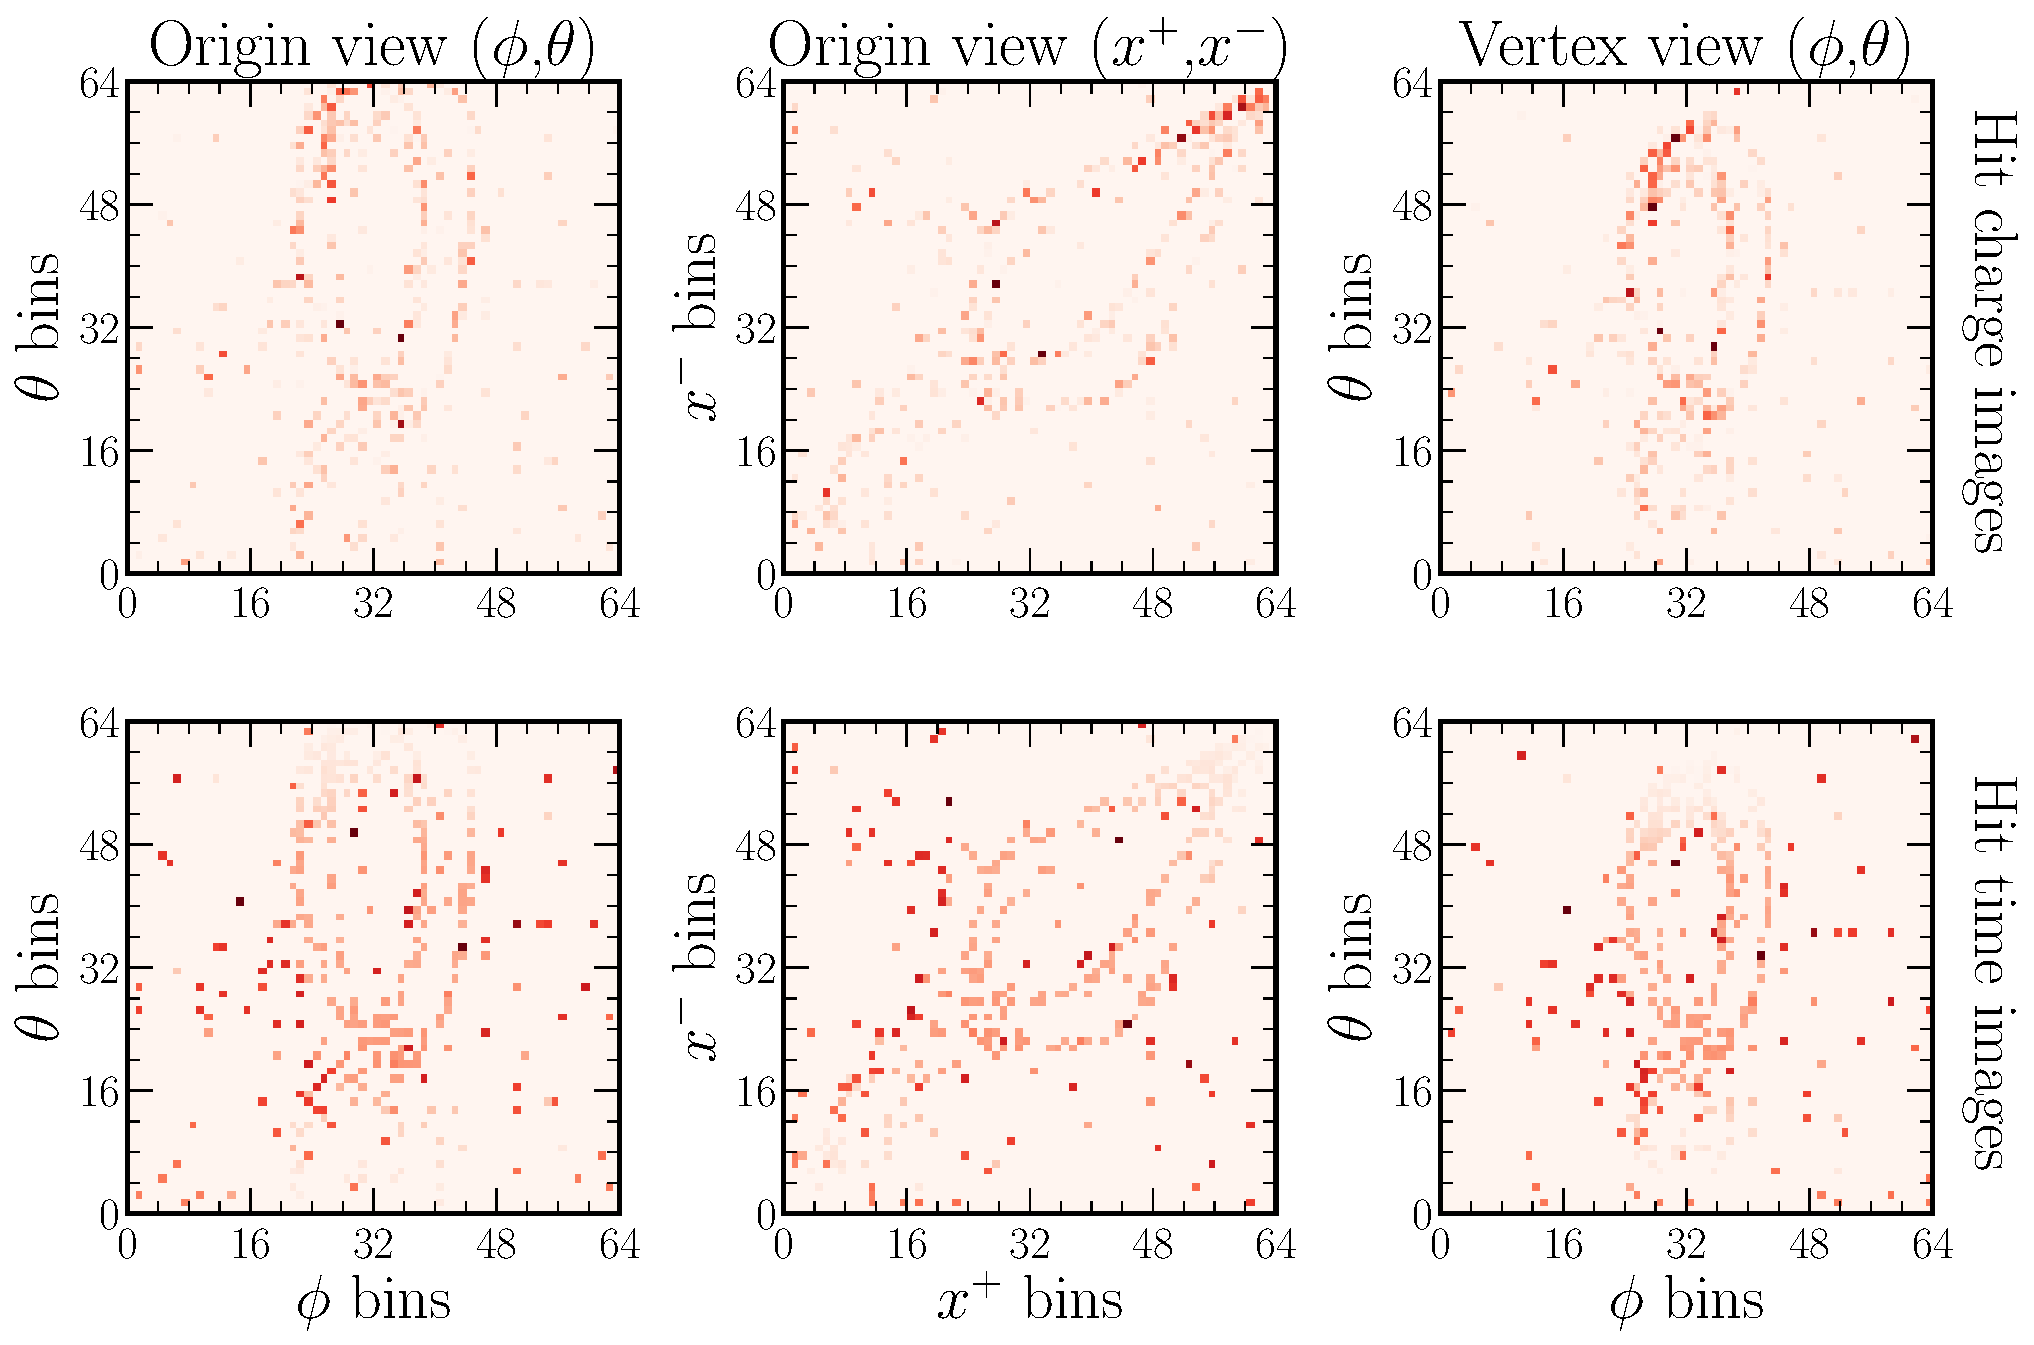
\includegraphics[width=0.8\textwidth]{diagrams/6-cvn/chipsnet/explore_nuel_ncdis_event.pdf}
    \caption[explore nuel ncdis event short]
    {92
    9301.59
    -1.0
    [  12 2212  211 2212 2212 2112 -999 -999 -999 -999 -999 -999 -999 -999
    -999 -999 -999 -999 -999 -999]
    [4731.25  2635.15  2511.54  1046.97   998.676  993.868 -999.    -999.
    -999.    -999.    -999.    -999.    -999.    -999.    -999.    -999.
    -999.    -999.    -999.    -999.   ]
    -1
    }
    \label{fig:explore_nuel_ncdis_event}
\end{figure}

\begin{figure} % COSMIC MUON EVENT DIAGRAM %
    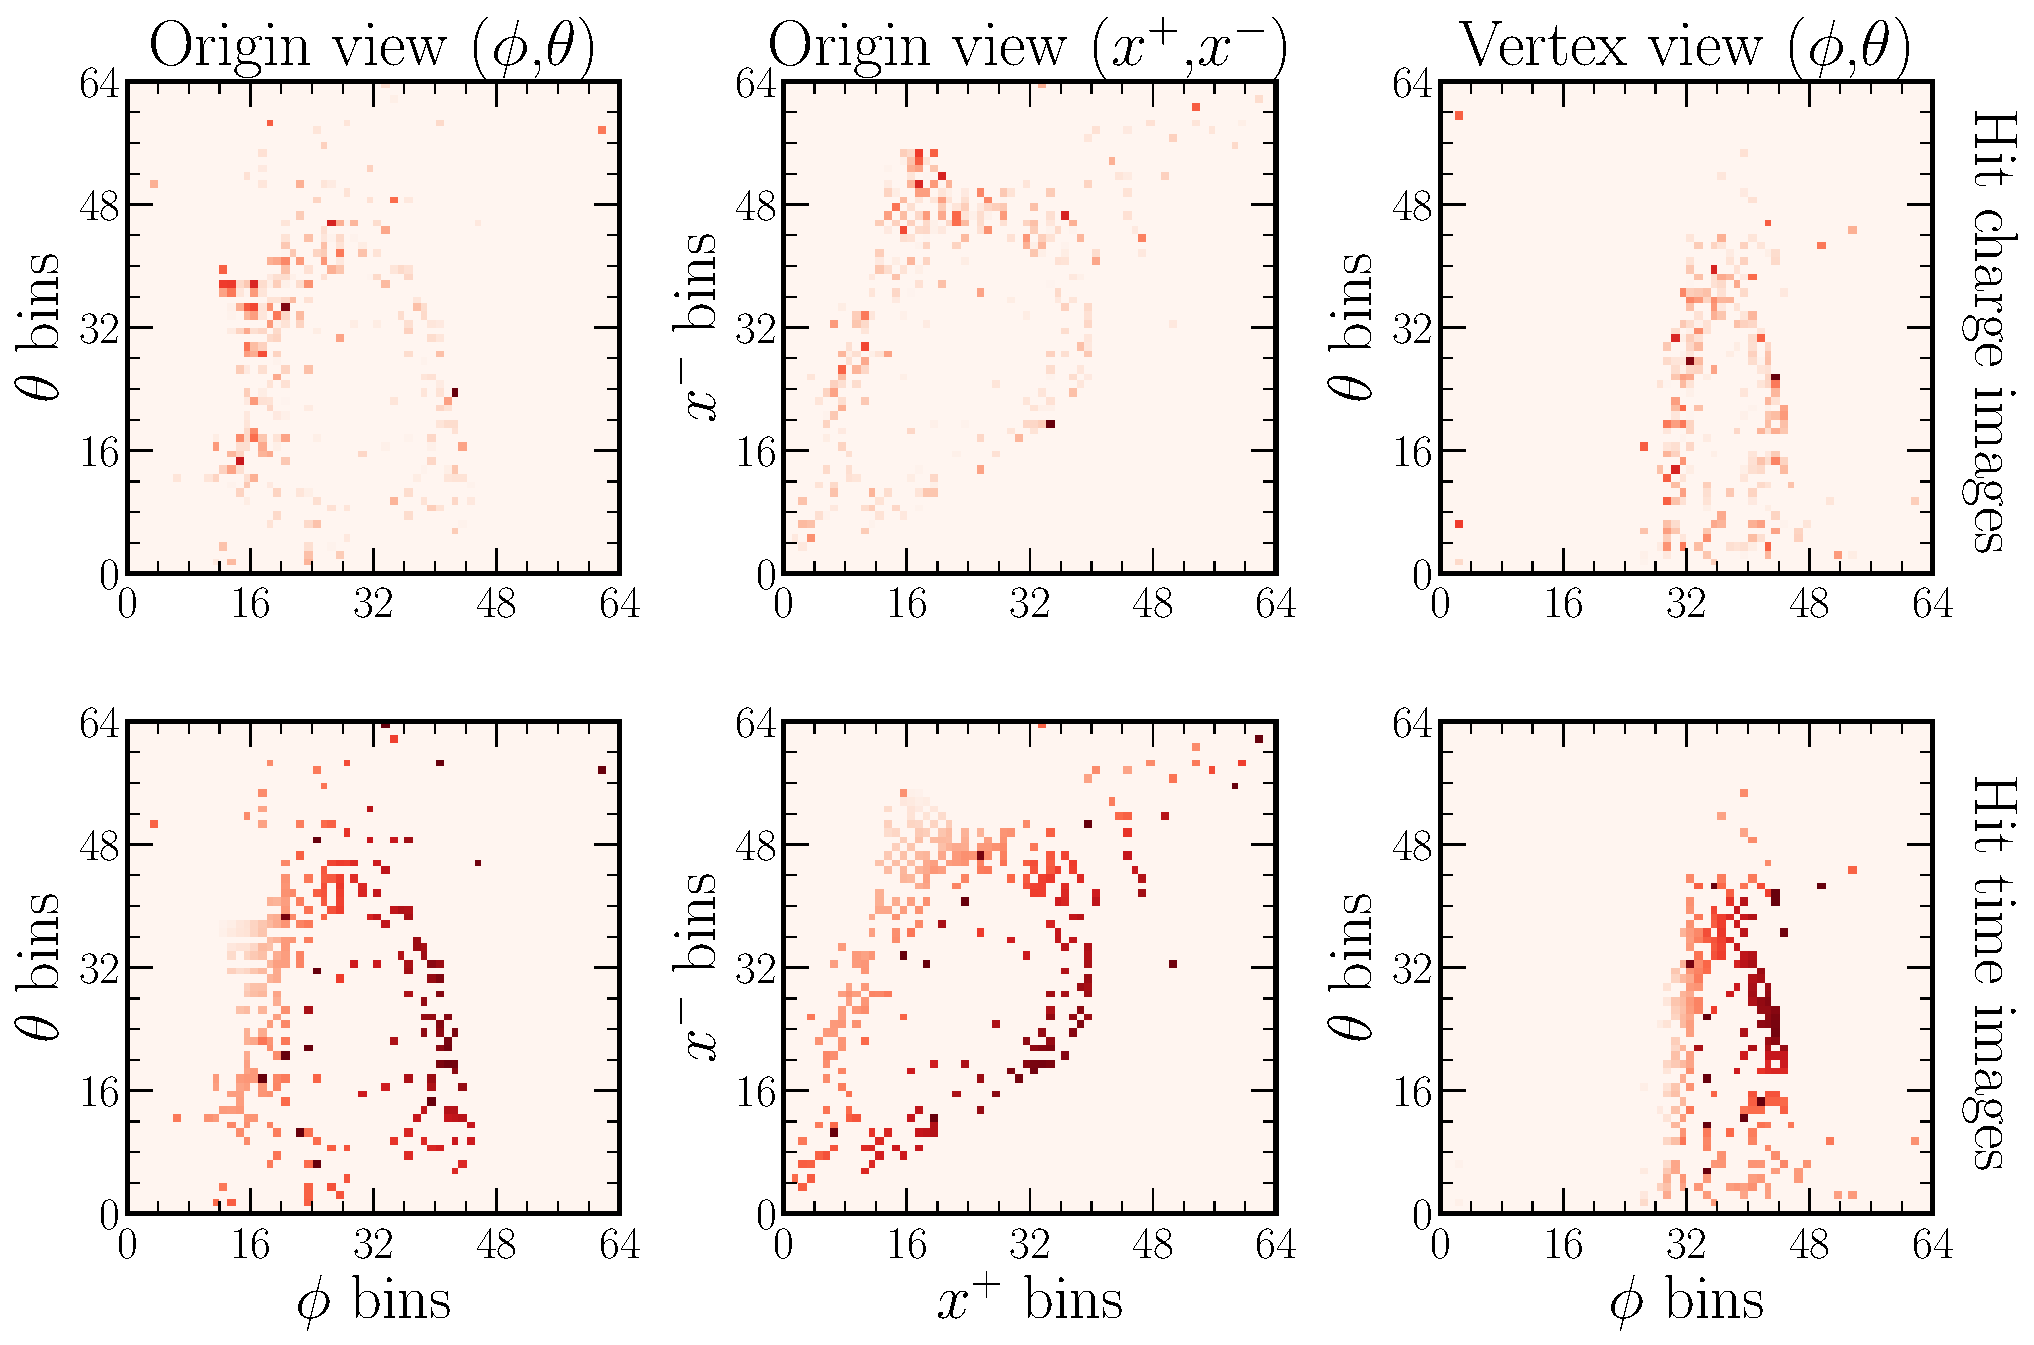
\includegraphics[width=0.8\textwidth]{diagrams/6-cvn/chipsnet/explore_cosmic_event.pdf}
    \caption[explore cosmic event short]
    {100
        2928.5
        2928.5
            [  13 -999 -999 -999 -999 -999 -999 -999 -999 -999 -999 -999 -999 -999
                -999 -999 -999 -999 -999 -999]
            [2928.5 -999.  -999.  -999.  -999.  -999.  -999.  -999.  -999.  -999.
                -999.  -999.  -999.  -999.  -999.  -999.  -999.  -999.  -999.  -999. ]
        0}
    \label{fig:explore_cosmic_event}
\end{figure}

\begin{figure} % HOUGH REPRESENTATIONS DIAGRAM %
    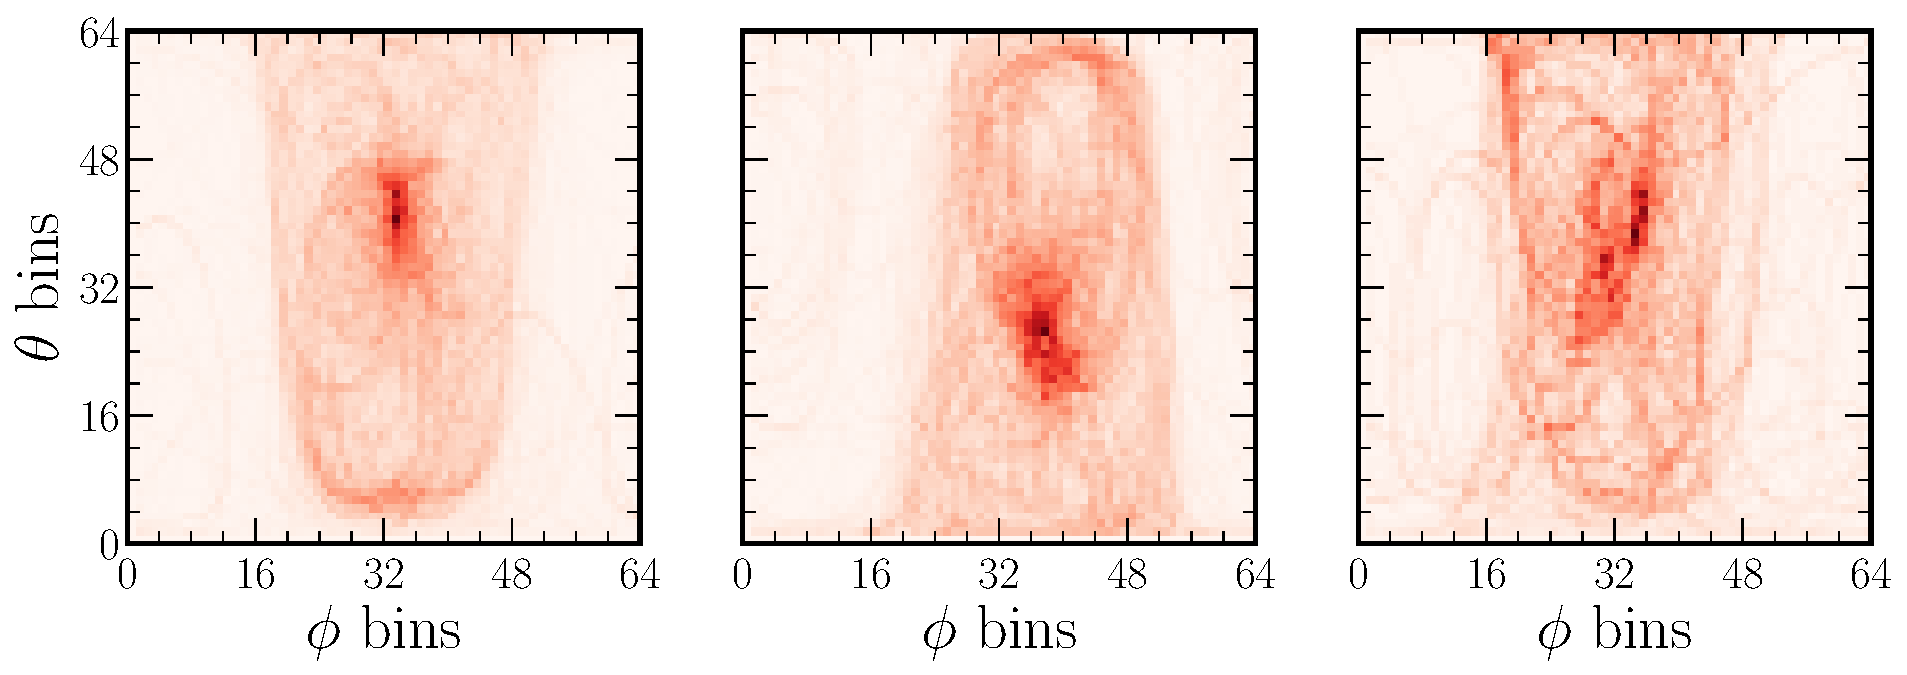
\includegraphics[width=\textwidth]{diagrams/6-cvn/chipsnet/explore_hough_events.pdf}
    \caption[example hough events short]
    {example hough events long}
    \label{fig:example_hough_events}
\end{figure}

\begin{figure} % VTX POSITIONS DIAGRAM %
    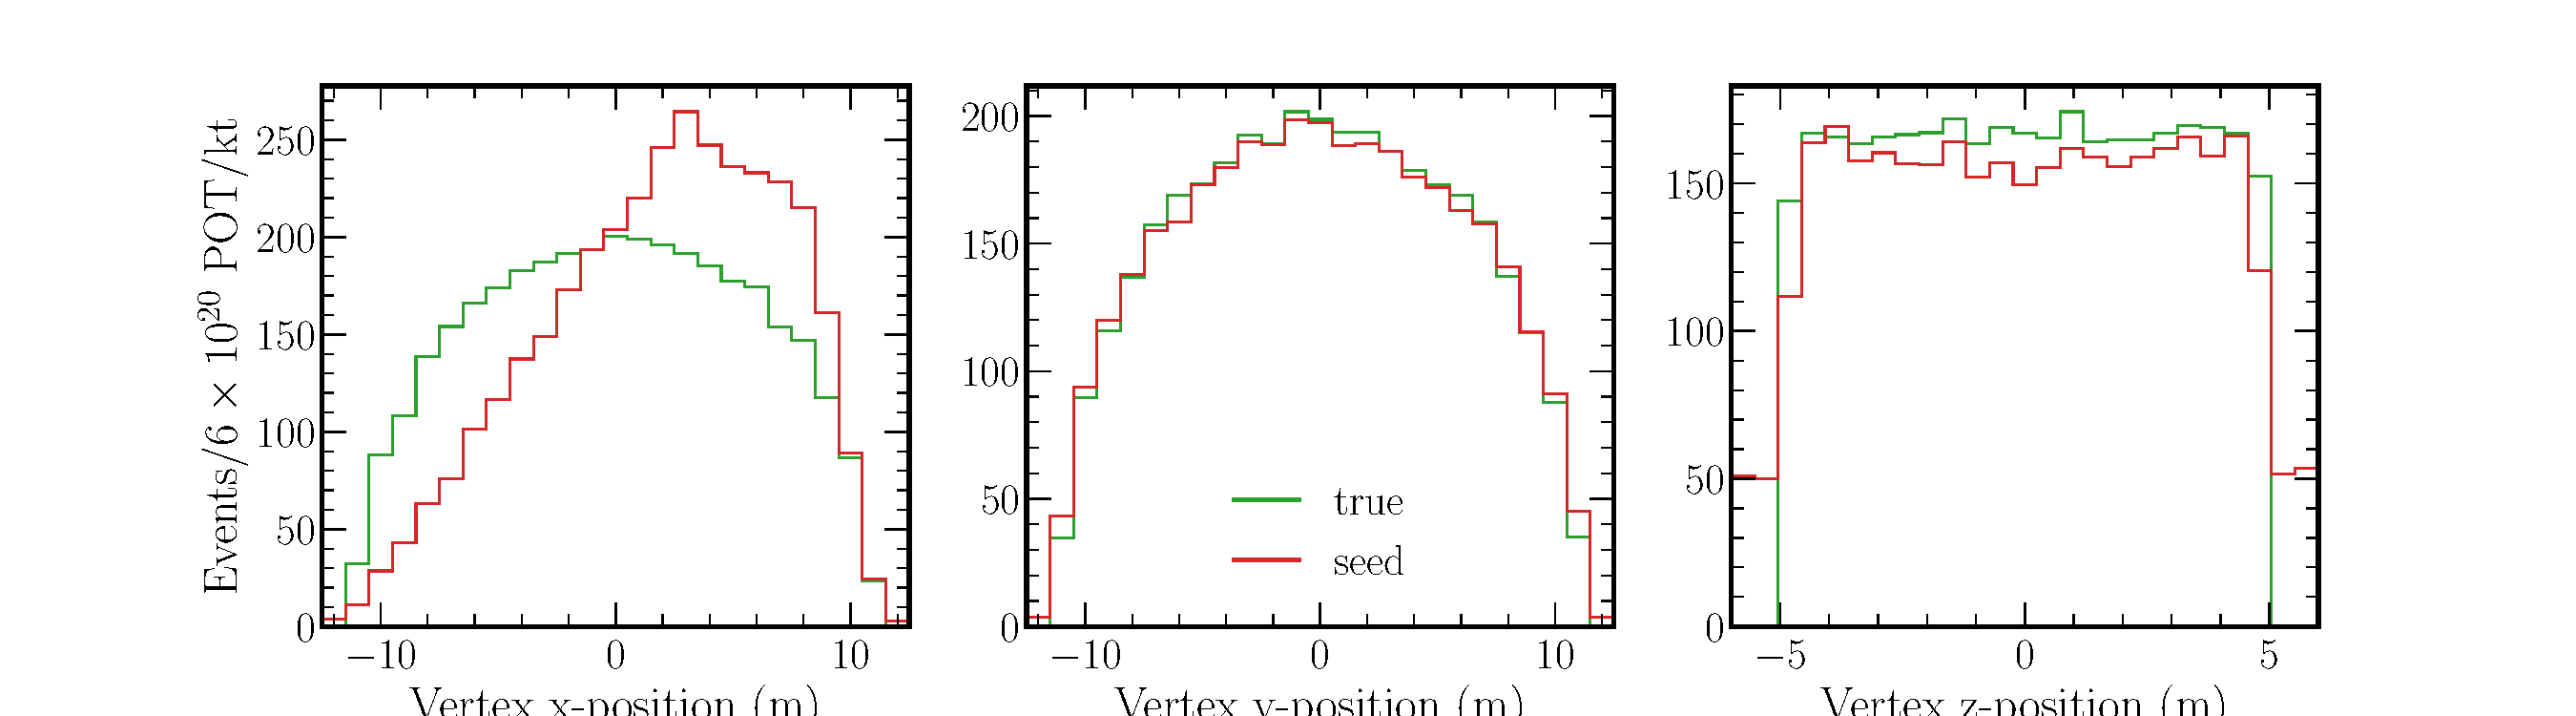
\includegraphics[width=\textwidth]{diagrams/6-cvn/chipsnet/explore_vtx_positions.pdf}
    \caption[explore vtx positions short]
    {explore vtx positions long}
    \label{fig:explore_vtx_positions}
\end{figure}

\begin{figure} % HOUGH VTX RES DIAGRAM %
    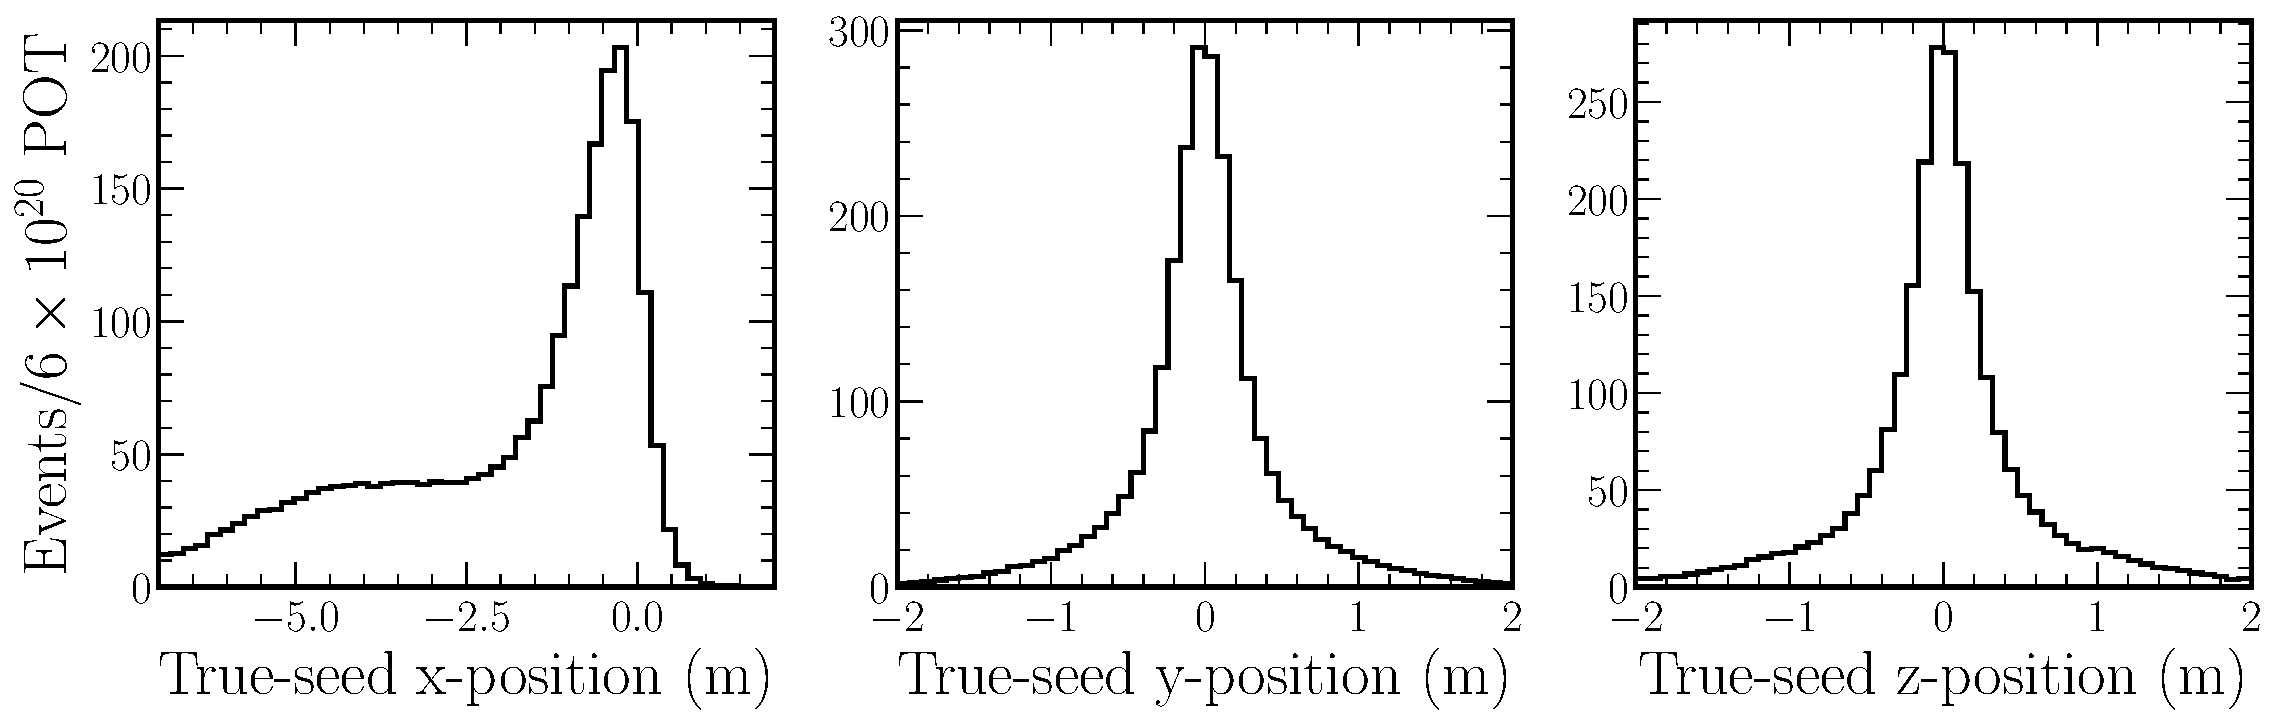
\includegraphics[width=\textwidth]{diagrams/6-cvn/chipsnet/explore_true_reco_vtx.pdf}
    \caption[explore true reco vtx short]
    {explore true reco vtx long}
    \label{fig:explore_true_reco_vtx}
\end{figure}

- Nuel-> ROC-AUC: 0.82509, PRC-AUC: 0.70686, S-Eff: 0.87786, S-Pur: 0.35433
- FOM1-> 0.46118, 0.93000, 52.98765, 8.61419, 15.27335, 0.66908, 0.68927
- FOM2-> 13.26595, 0.98500, 29.74203, 1.43964, 3.58684, 0.37556, 0.85543

- Nuel-> ROC-AUC: 0.82178, PRC-AUC: 0.67486, S-Eff: 0.87439, S-Pur: 0.29114
- FOM1-> 0.42202, 0.95500, 50.65626, 10.27209, 15.82963, 0.63948, 0.65995
- FOM2-> 12.53864, 0.99000, 29.40728, 1.75353, 3.74706, 0.37123, 0.84243

- Nuel-> ROC-AUC: 0.82116, PRC-AUC: 0.66987, S-Eff: 0.86660, S-Pur: 0.29764
- FOM1-> 0.41895, 0.94500, 50.97483, 10.86474, 16.45768, 0.64350, 0.65104
- FOM2-> 12.22739, 0.99000, 28.43808, 1.74364, 3.66555, 0.35900, 0.84019

\begin{figure} % REPR NUEL EFF CURVES DIAGRAM %
    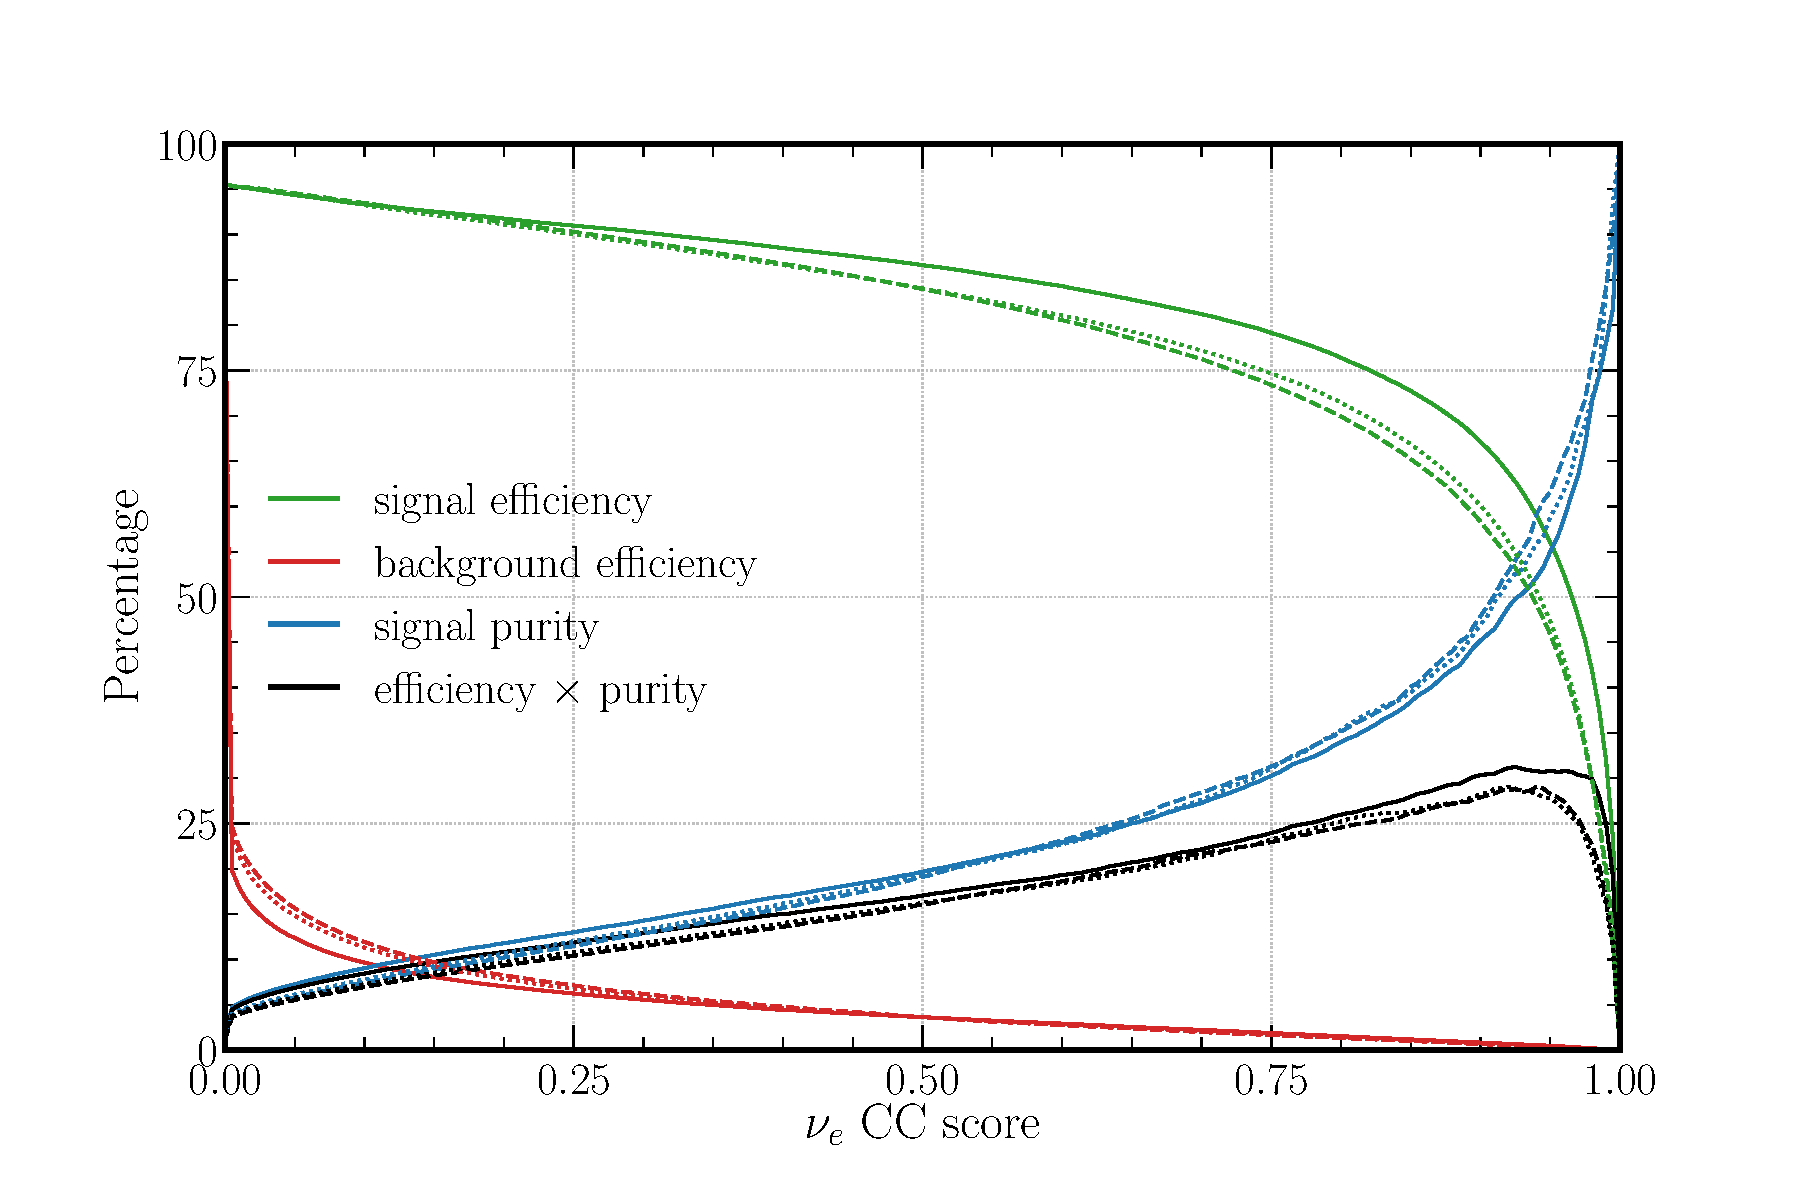
\includegraphics[width=0.6\textwidth]{diagrams/6-cvn/chipsnet/repr_nuel_eff_curves.pdf}
    \caption[repr nuel eff curves short]
    {v=solid, o=dashed, i=dotted}
    \label{fig:repr_nuel_eff_curves}
\end{figure}

\begin{figure} % REPR NUEL COMP CURVES DIAGRAM %
    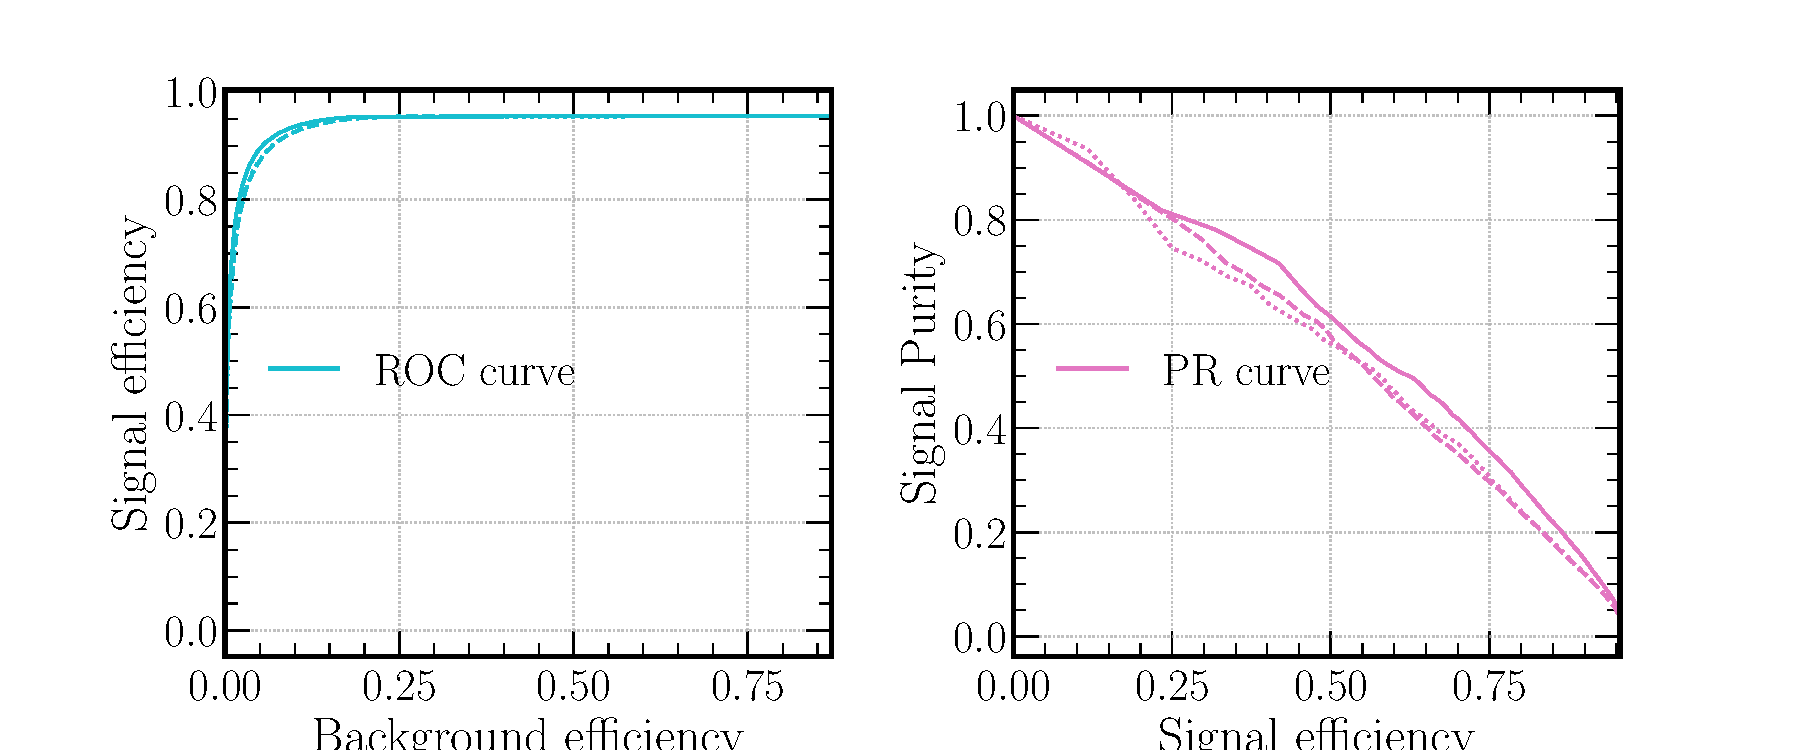
\includegraphics[width=0.8\textwidth]{diagrams/6-cvn/chipsnet/repr_nuel_comp_curves.pdf}
    \caption[repr nuel comp curves short]
    {v=solid, o=dashed, i=dotted}
    \label{fig:repr_nuel_comp_curves}
\end{figure}

\begin{figure} % REPR NUMU EFF CURVES DIAGRAM %
    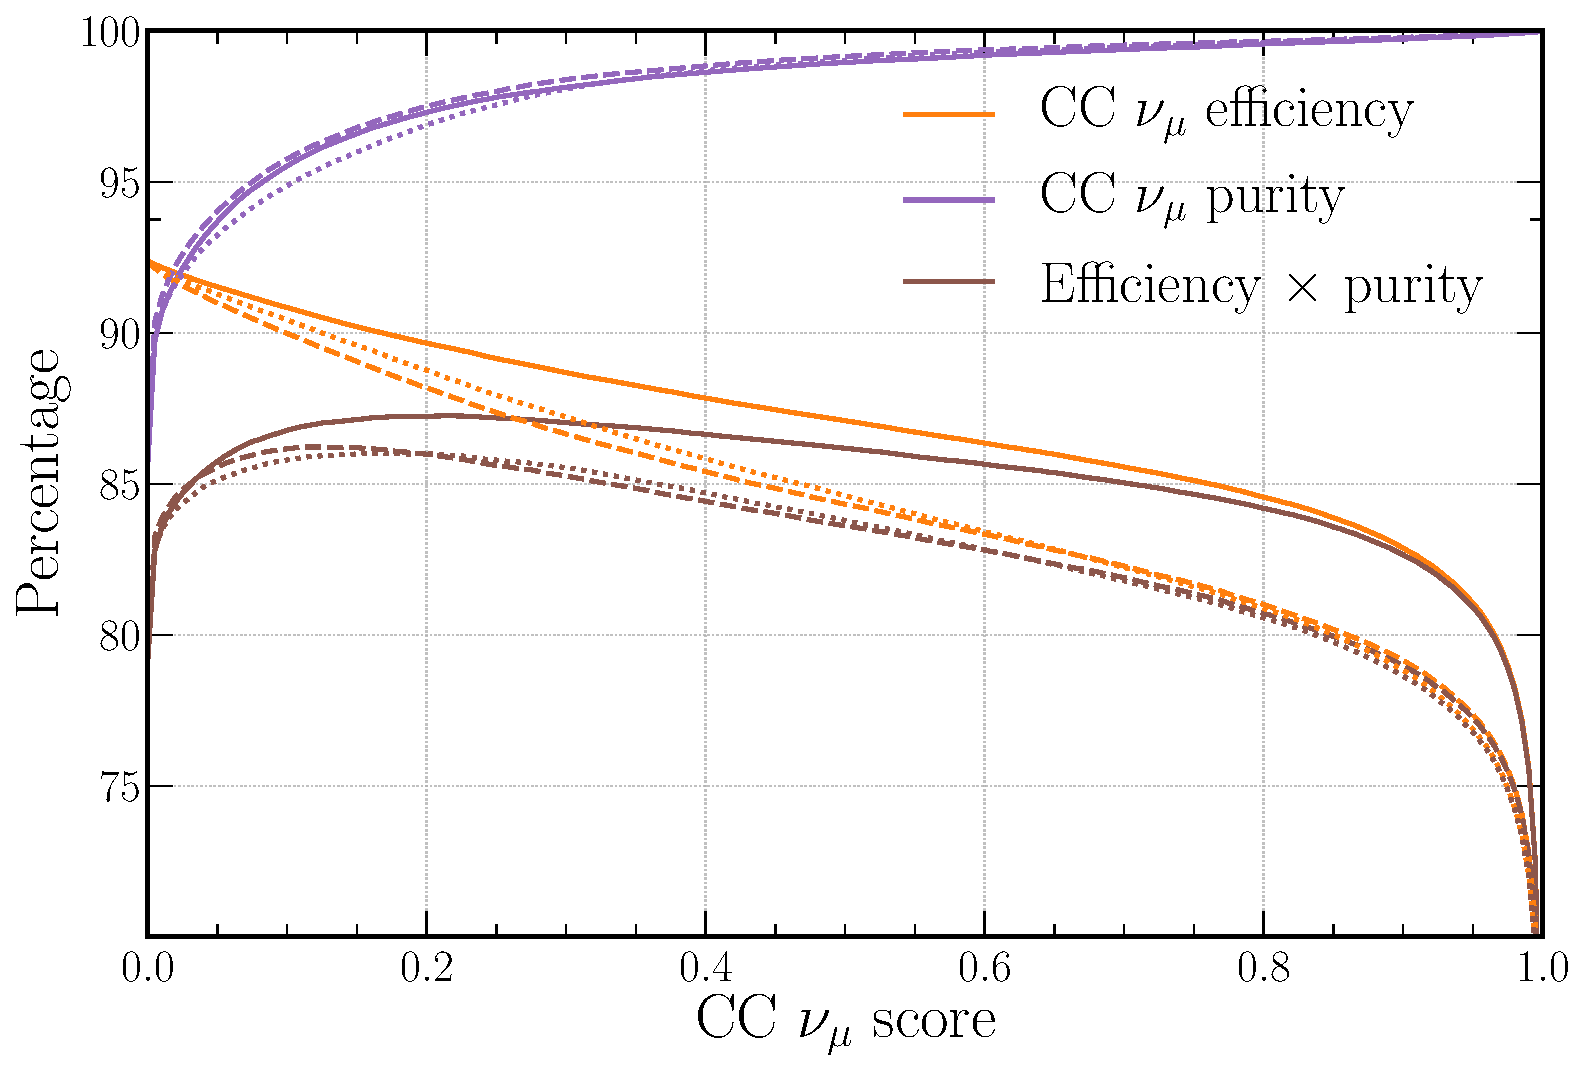
\includegraphics[width=0.6\textwidth]{diagrams/6-cvn/chipsnet/repr_numu_eff_curves.pdf}
    \caption[repr numu eff curves short]
    {v=solid, o=dashed, i=dotted}
    \label{fig:repr_numu_eff_curves}
\end{figure}

\begin{figure} % REPR NUMU COMP CURVES DIAGRAM %
    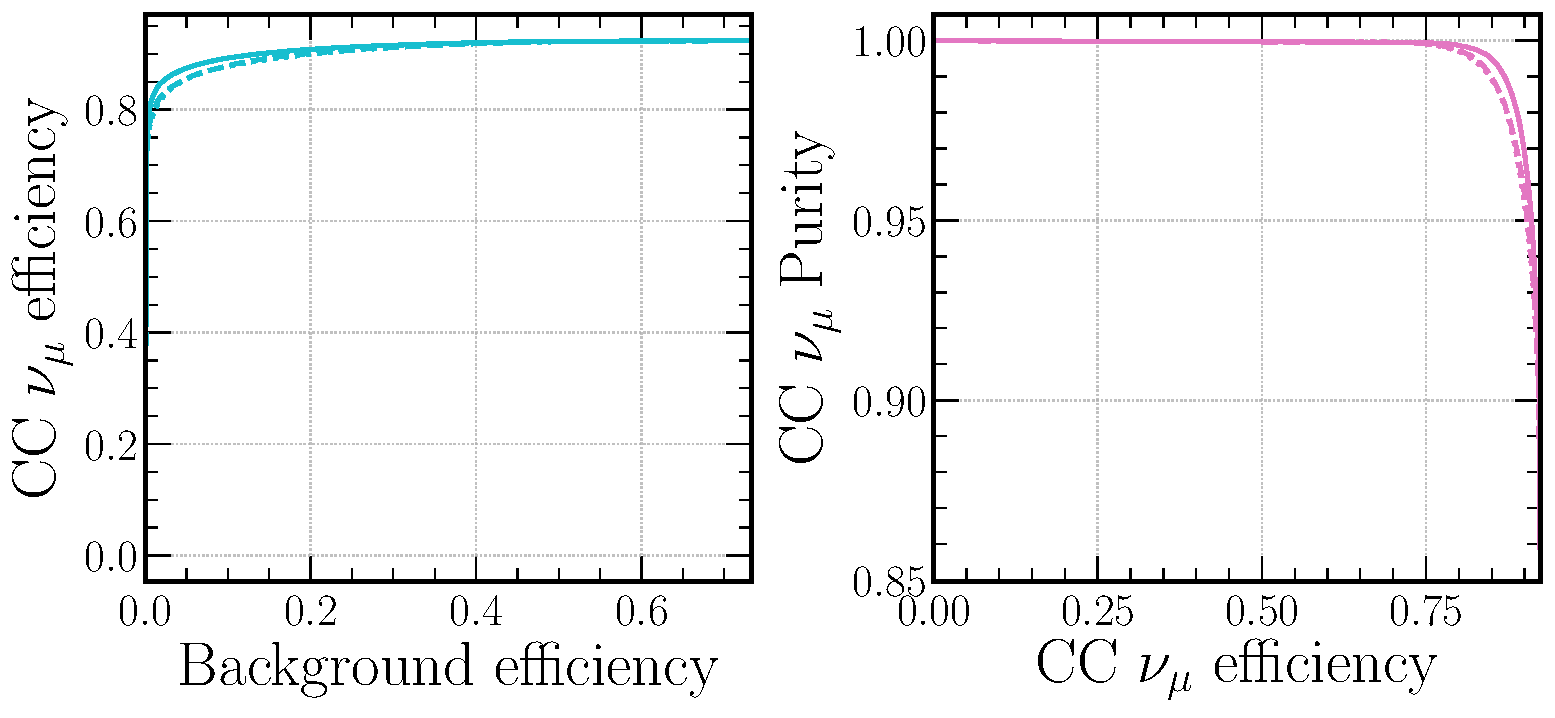
\includegraphics[width=0.8\textwidth]{diagrams/6-cvn/chipsnet/repr_numu_comp_curves.pdf}
    \caption[repr numu comp curves short]
    {v=solid, o=dashed, i=dotted}
    \label{fig:repr_numu_comp_curves}
\end{figure}

\subsection{Which channels to use} %%%%%%%%%%%%%%%%%%%%%%%%%%%%%%%%%%%%%%%%%%%%%%%%%%%%%%%%%%%%%%%
\label{sec:cvn_baseline_channel} %%%%%%%%%%%%%%%%%%%%%%%%%%%%%%%%%%%%%%%%%%%%%%%%%%%%%%%%%%%%%%%%%

\begin{figure} % CHANNEL NUEL EFF CURVES DIAGRAM %
    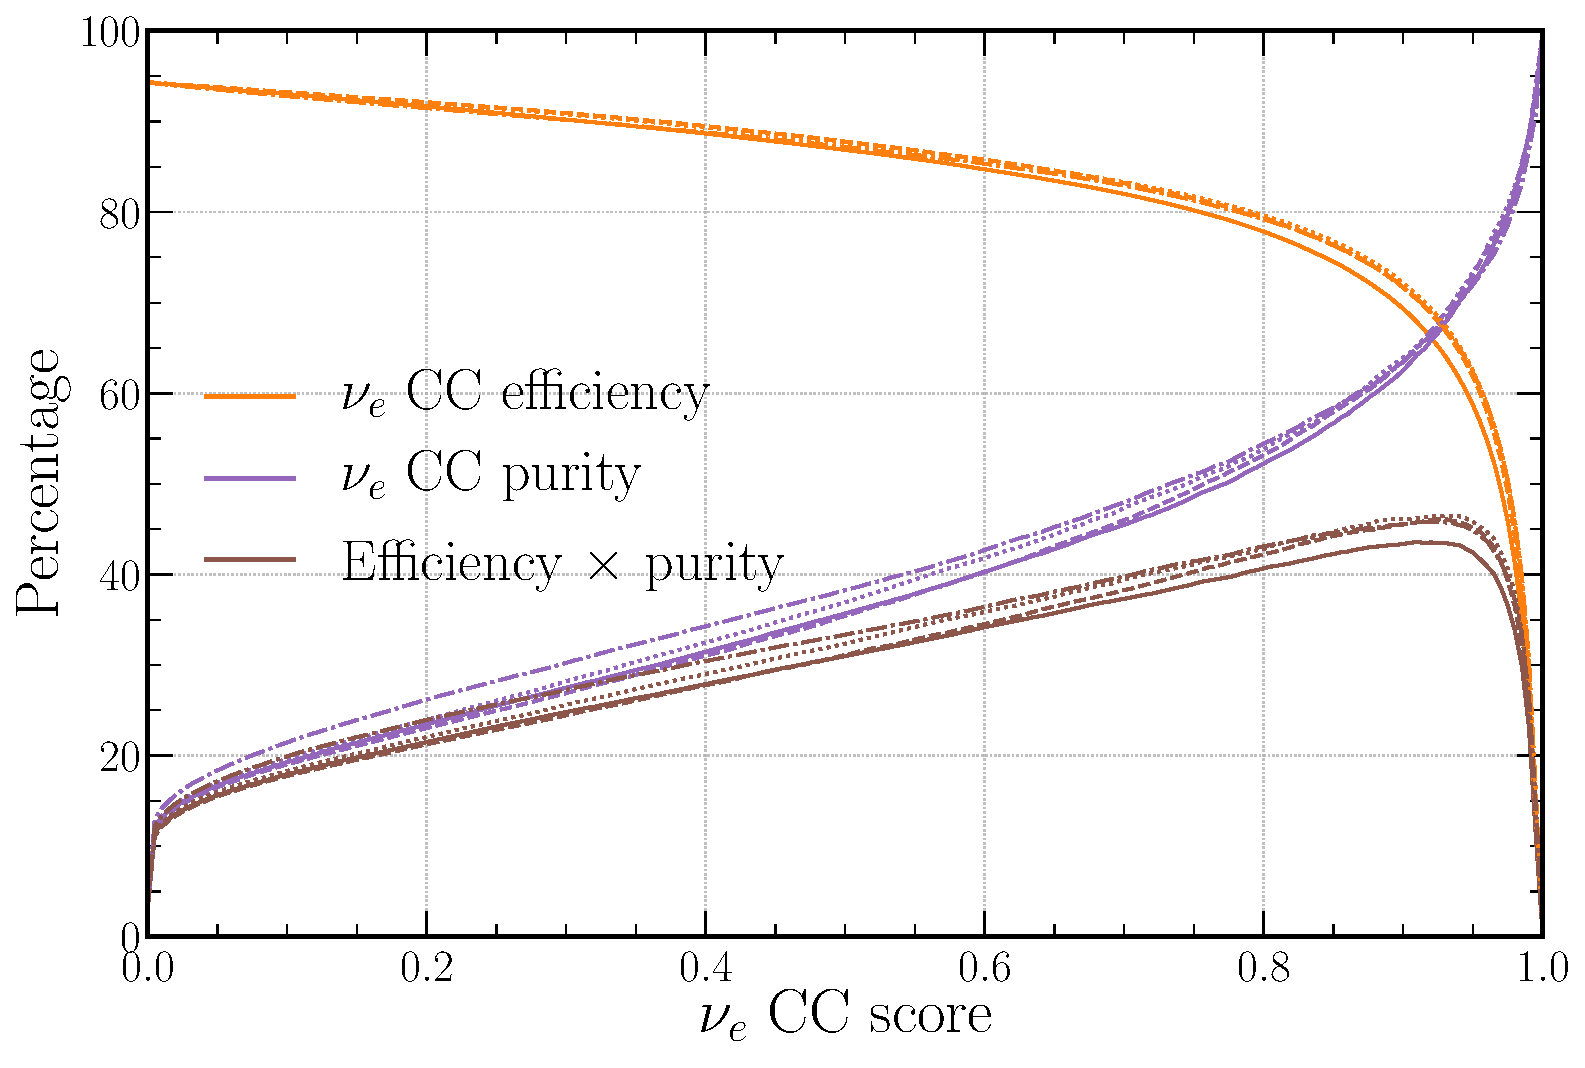
\includegraphics[width=0.6\textwidth]{diagrams/6-cvn/chipsnet/channel_nuel_eff_curves.pdf}
    \caption[channel nuel eff curves short]
    {c=solid, ct=dashed, cth=dotted, cth-stacked=dot-dash}
    \label{fig:channel_nuel_eff_curves}
\end{figure}

\begin{figure} % CHANNEL NUEL COMP CURVES DIAGRAM %
    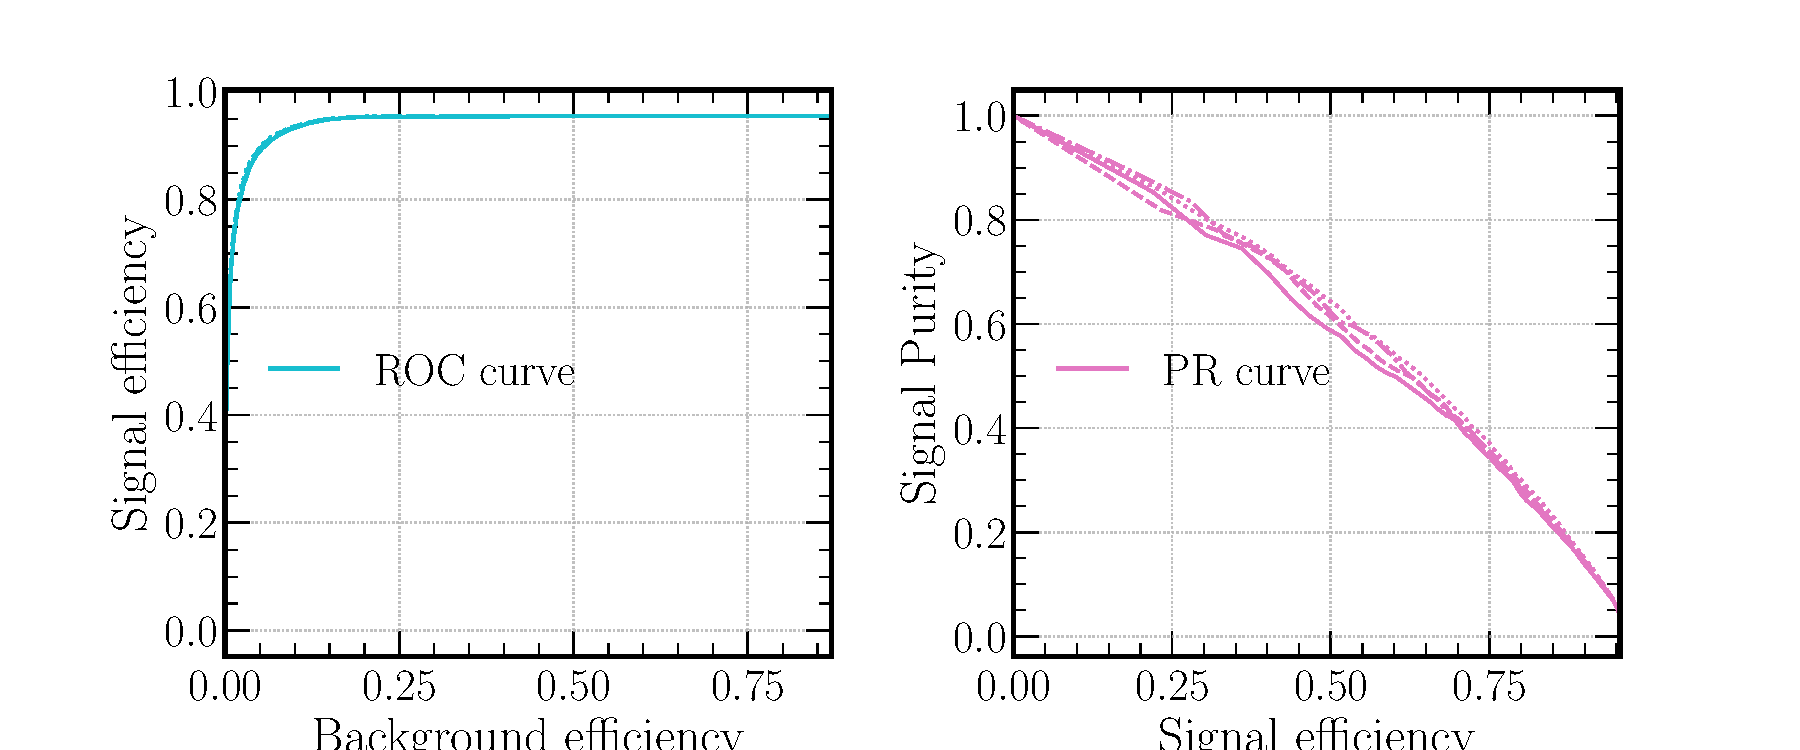
\includegraphics[width=0.8\textwidth]{diagrams/6-cvn/chipsnet/channel_nuel_comp_curves.pdf}
    \caption[channel nuel comp curves short]
    {c=solid, ct=dashed, cth=dotted, cth-stacked=dot-dash}
    \label{fig:channel_nuel_comp_curves}
\end{figure}

- Nuel-> ROC-AUC: 0.82377, PRC-AUC: 0.68935, S-Eff: 0.86860, S-Pur: 0.35681
- FOM1-> 0.43601, 0.91000, 53.71070, 12.22704, 17.60798, 0.67821, 0.64289
- FOM2-> 12.70378, 0.99000, 20.73912, 0.76294, 1.90217, 0.26187, 0.88613

- Nuel-> ROC-AUC: 0.82509, PRC-AUC: 0.70686, S-Eff: 0.87786, S-Pur: 0.35433
- FOM1-> 0.46118, 0.93000, 52.98765, 8.61419, 15.27335, 0.66908, 0.68927
- FOM2-> 13.26595, 0.98500, 29.74203, 1.43964, 3.58684, 0.37556, 0.85543

- Nuel-> ROC-AUC: 0.82559, PRC-AUC: 0.71155, S-Eff: 0.87661, S-Pur: 0.36928
- FOM1-> 0.46510, 0.93000, 53.44422, 8.34671, 15.75487, 0.67485, 0.68920
- FOM2-> 13.44645, 0.98500, 31.21664, 1.57028, 3.81933, 0.39418, 0.85277

- Nuel-> ROC-AUC: 0.82521, PRC-AUC: 0.70198, S-Eff: 0.87180, S-Pur: 0.38254
- FOM1-> 0.45819, 0.91500, 55.18628, 11.56662, 17.17741, 0.69684, 0.65753
- FOM2-> 12.66558, 0.99000, 24.37959, 1.35104, 2.35408, 0.30784, 0.86807

\begin{figure} % CHANNEL NUMU EFF CURVES DIAGRAM %
    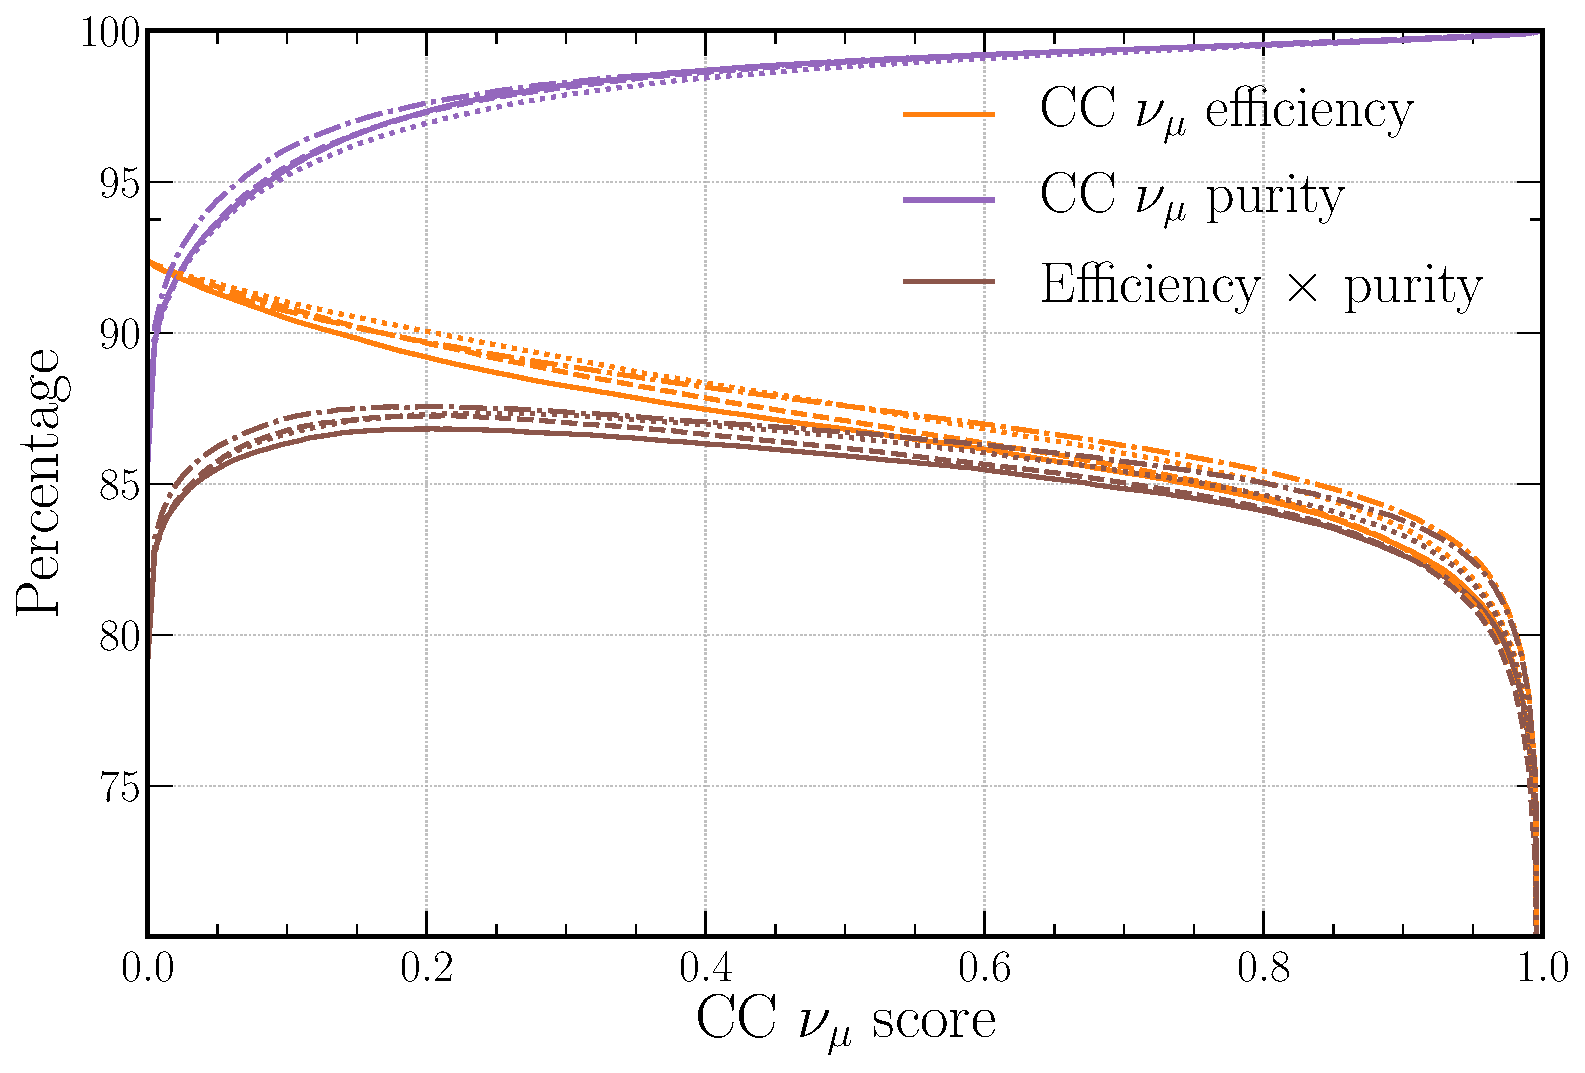
\includegraphics[width=0.6\textwidth]{diagrams/6-cvn/chipsnet/channel_numu_eff_curves.pdf}
    \caption[channel numu eff curves short]
    {c=solid, ct=dashed, cth=dotted, cth-stacked=dot-dash}
    \label{fig:channel_numu_eff_curves}
\end{figure}

\begin{figure} % CHANNEL NUMU COMP CURVES DIAGRAM %
    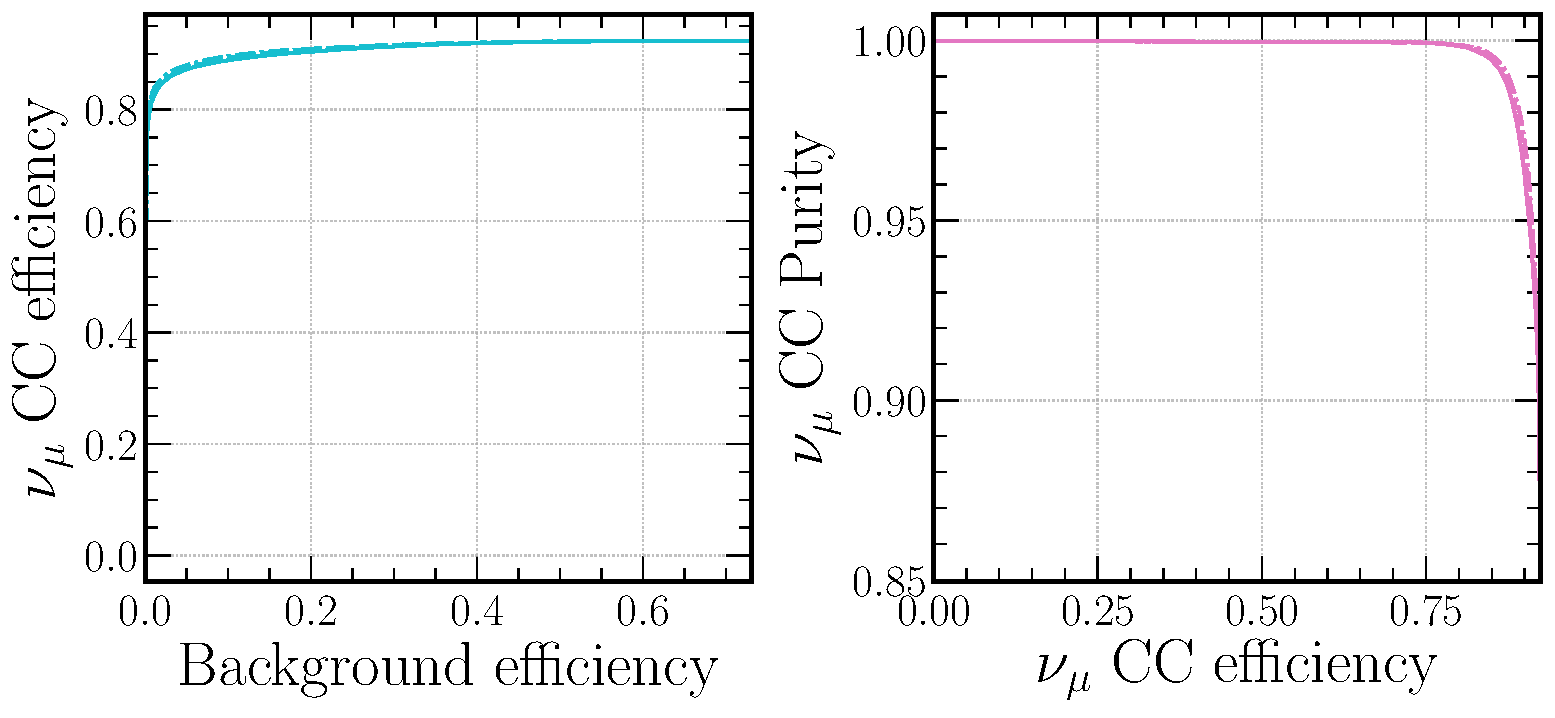
\includegraphics[width=0.8\textwidth]{diagrams/6-cvn/chipsnet/channel_numu_comp_curves.pdf}
    \caption[channel numu comp curves short]
    {c=solid, ct=dashed, cth=dotted, cth-stacked=dot-dash}
    \label{fig:channel_numu_comp_curves}
\end{figure}

\subsection{Multitask methodology} %%%%%%%%%%%%%%%%%%%%%%%%%%%%%%%%%%%%%%%%%%%%%%%%%%%%%%%%%%%%%%%
\label{sec:cvn_baseline_multi} %%%%%%%%%%%%%%%%%%%%%%%%%%%%%%%%%%%%%%%%%%%%%%%%%%%%%%%%%%%%%%%%%%%

Multi-task learning how to weight paper in Ref.~\cite{kendall2018}

\section{Cosmic muon rejection} %%%%%%%%%%%%%%%%%%%%%%%%%%%%%%%%%%%%%%%%%%%%%%%%%%%%%%%%%%%%%%%%%%
\label{sec:cvn_cosmic} %%%%%%%%%%%%%%%%%%%%%%%%%%%%%%%%%%%%%%%%%%%%%%%%%%%%%%%%%%%%%%%%%%%%%%%%%%%

\section{Beam classification} %%%%%%%%%%%%%%%%%%%%%%%%%%%%%%%%%%%%%%%%%%%%%%%%%%%%%%%%%%%%%%%%%%%%
\label{sec:cvn_beam} %%%%%%%%%%%%%%%%%%%%%%%%%%%%%%%%%%%%%%%%%%%%%%%%%%%%%%%%%%%%%%%%%%%%%%%%%%%%%

\subsection{Which categorisation to use} %%%%%%%%%%%%%%%%%%%%%%%%%%%%%%%%%%%%%%%%%%%%%%%%%%%%%%%%%
\label{sec:cvn_beam_cat} %%%%%%%%%%%%%%%%%%%%%%%%%%%%%%%%%%%%%%%%%%%%%%%%%%%%%%%%%%%%%%%%%%%%%%%%%

\begin{figure} % T_ALL_CAT SAMPLE DIAGRAM %
    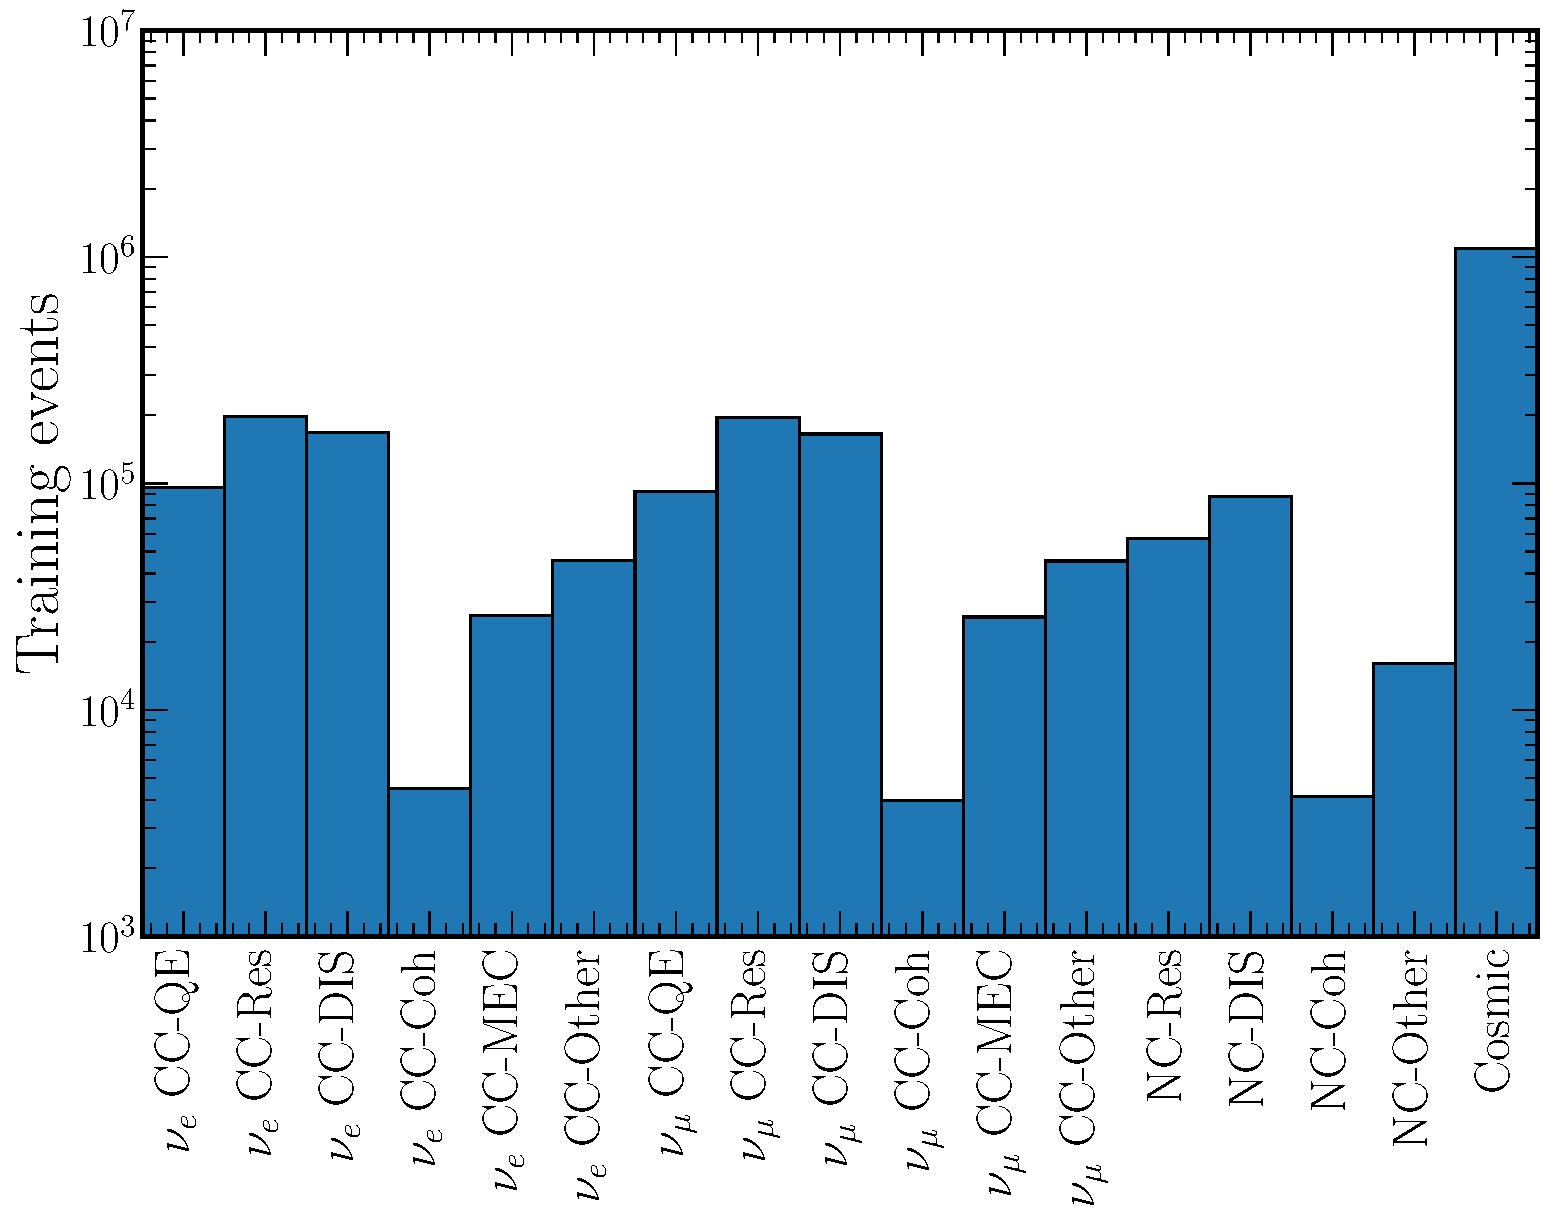
\includegraphics[width=0.6\textwidth]{diagrams/6-cvn/chipsnet/explore_t_all_cat.pdf}
    \caption[explore t all cat short]
    {explore t all cat long}
    \label{fig:explore_t_all_cat}
\end{figure}

\begin{figure} % T_NC_COMB_CAT SAMPLE DIAGRAM %
    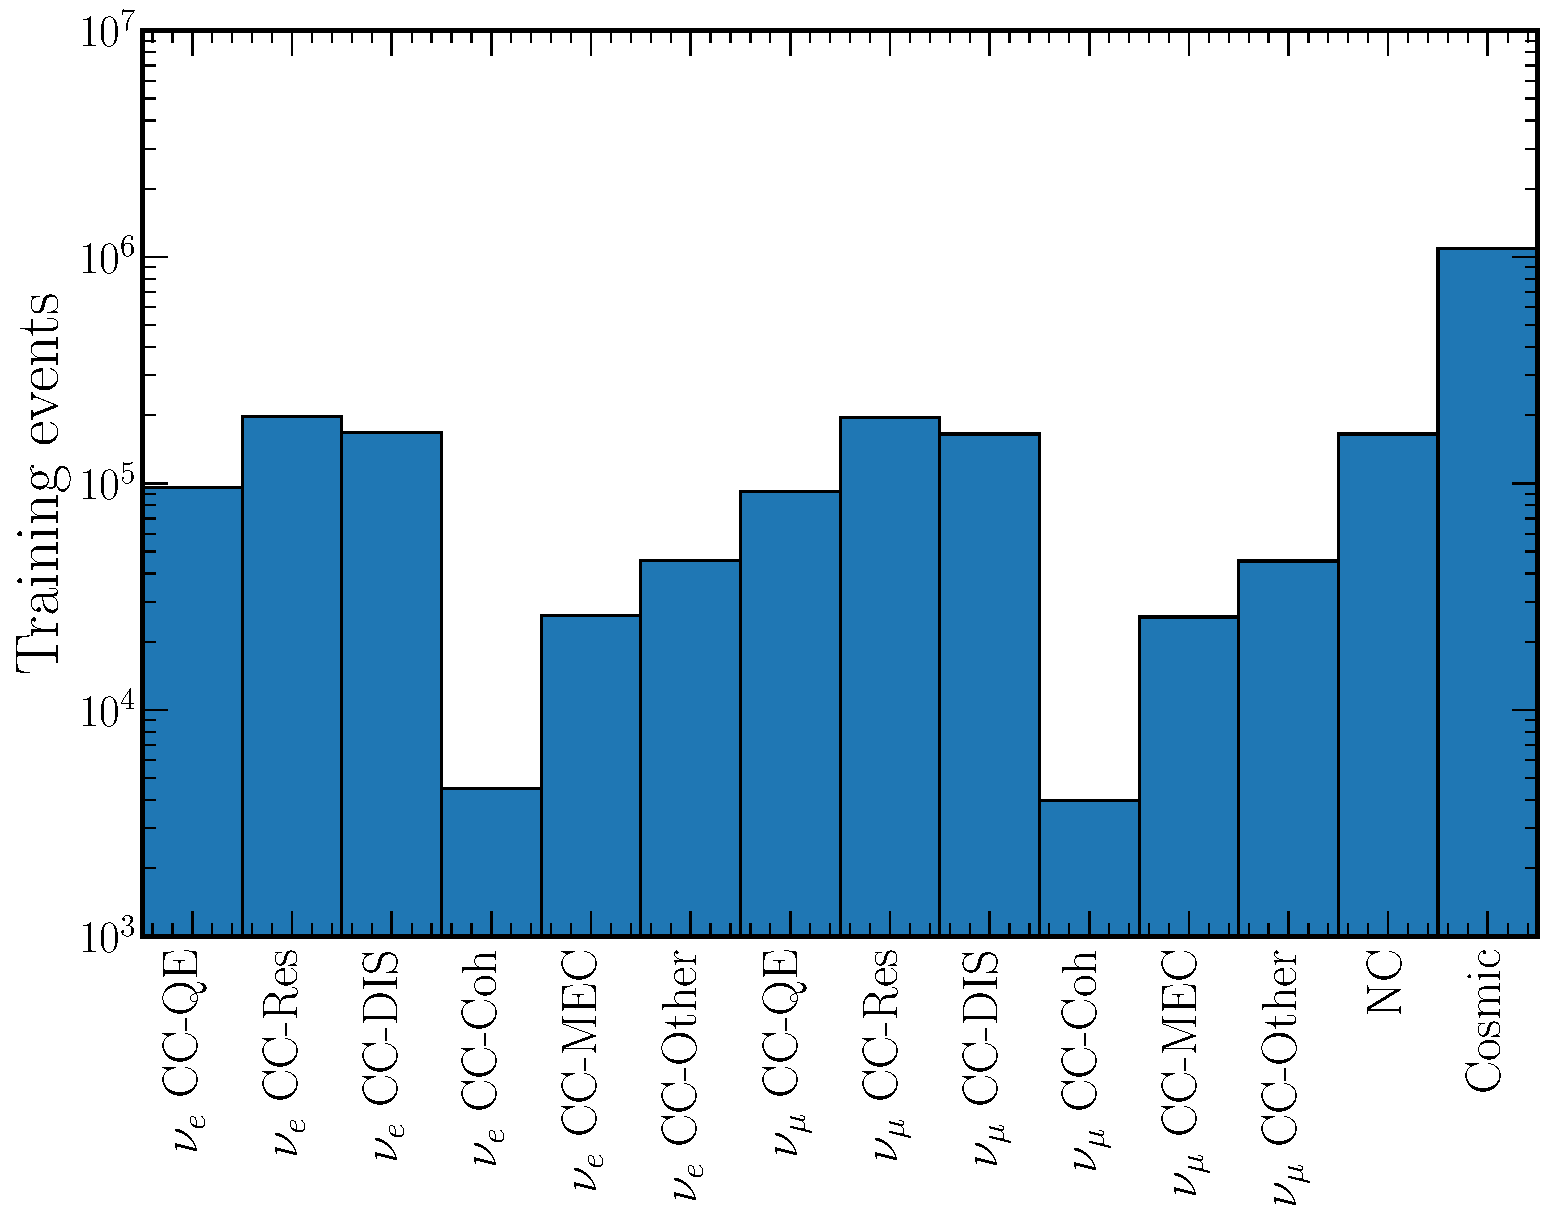
\includegraphics[width=0.6\textwidth]{diagrams/6-cvn/chipsnet/explore_t_nc_comb_cat.pdf}
    \caption[explore t nc comb cat short]
    {explore t nc comb cat long}
    \label{fig:explore_t_nc_comb_cat}
\end{figure}

\begin{figure} % T_COMB_CAT SAMPLE DIAGRAM %
    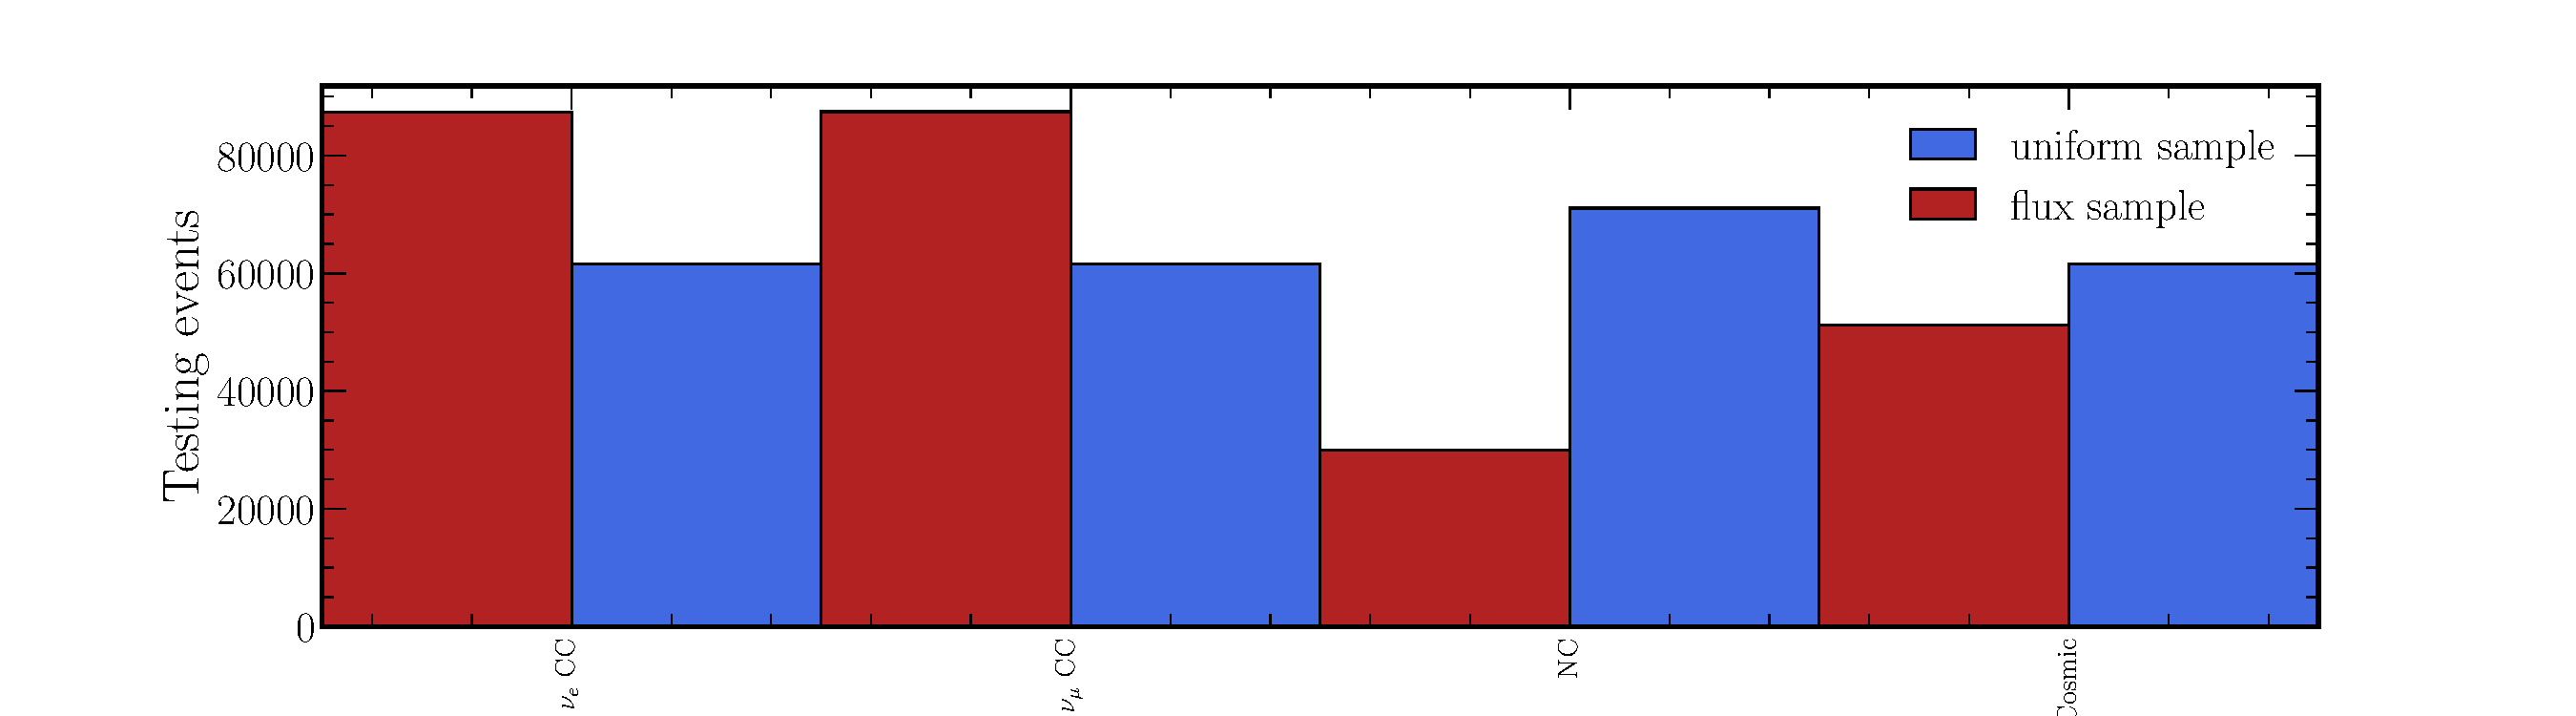
\includegraphics[width=0.6\textwidth]{diagrams/6-cvn/chipsnet/explore_t_comb_cat.pdf}
    \caption[explore t comb cat short]
    {explore t comb cat long}
    \label{fig:explore_t_comb_cat}
\end{figure}

\begin{figure} % CAT NUEL EFF CURVES DIAGRAM %
    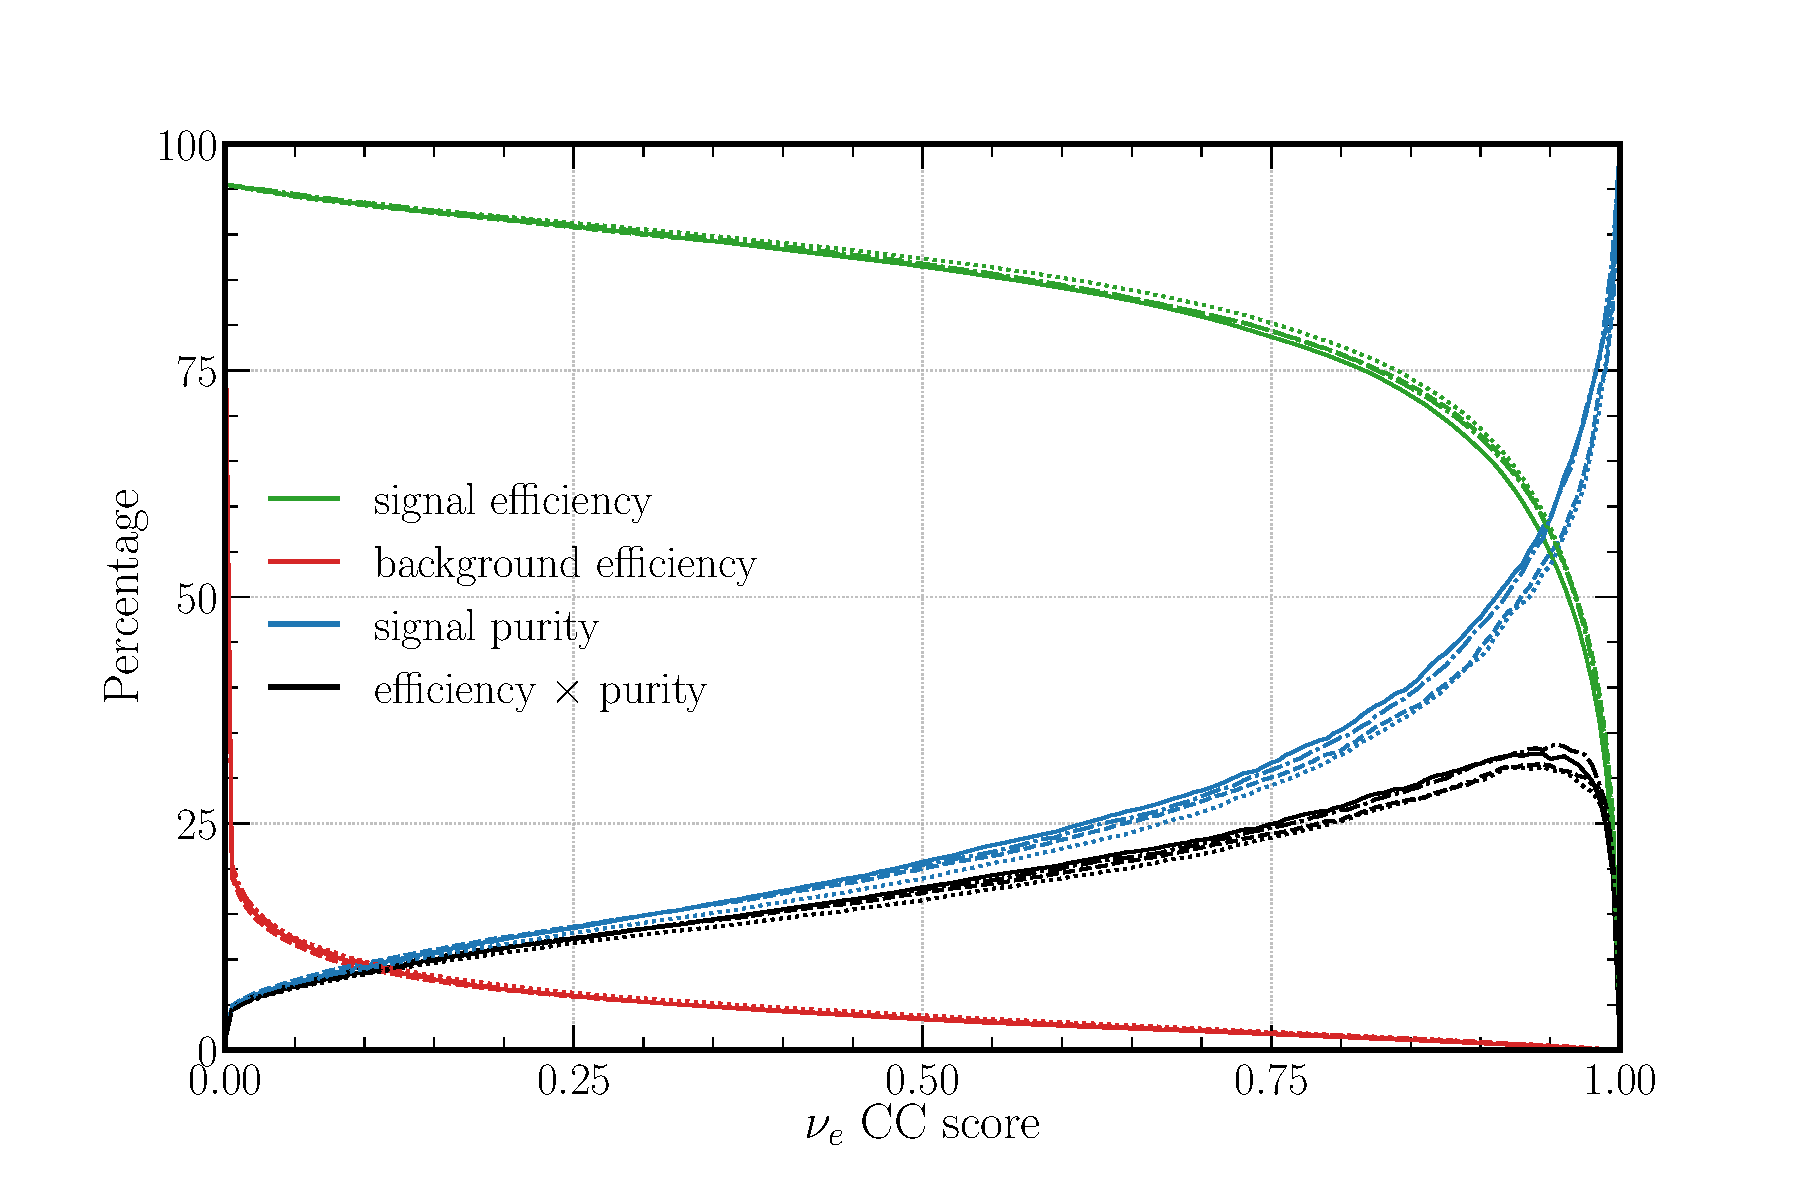
\includegraphics[width=0.6\textwidth]{diagrams/6-cvn/chipsnet/cat_nuel_eff_curves.pdf}
    \caption[cat nuel eff curves short]
    {cat nuel eff curves long}
    \label{fig:cat_nuel_eff_curves}
\end{figure}

\begin{figure} % CAT NUEL COMP CURVES DIAGRAM %
    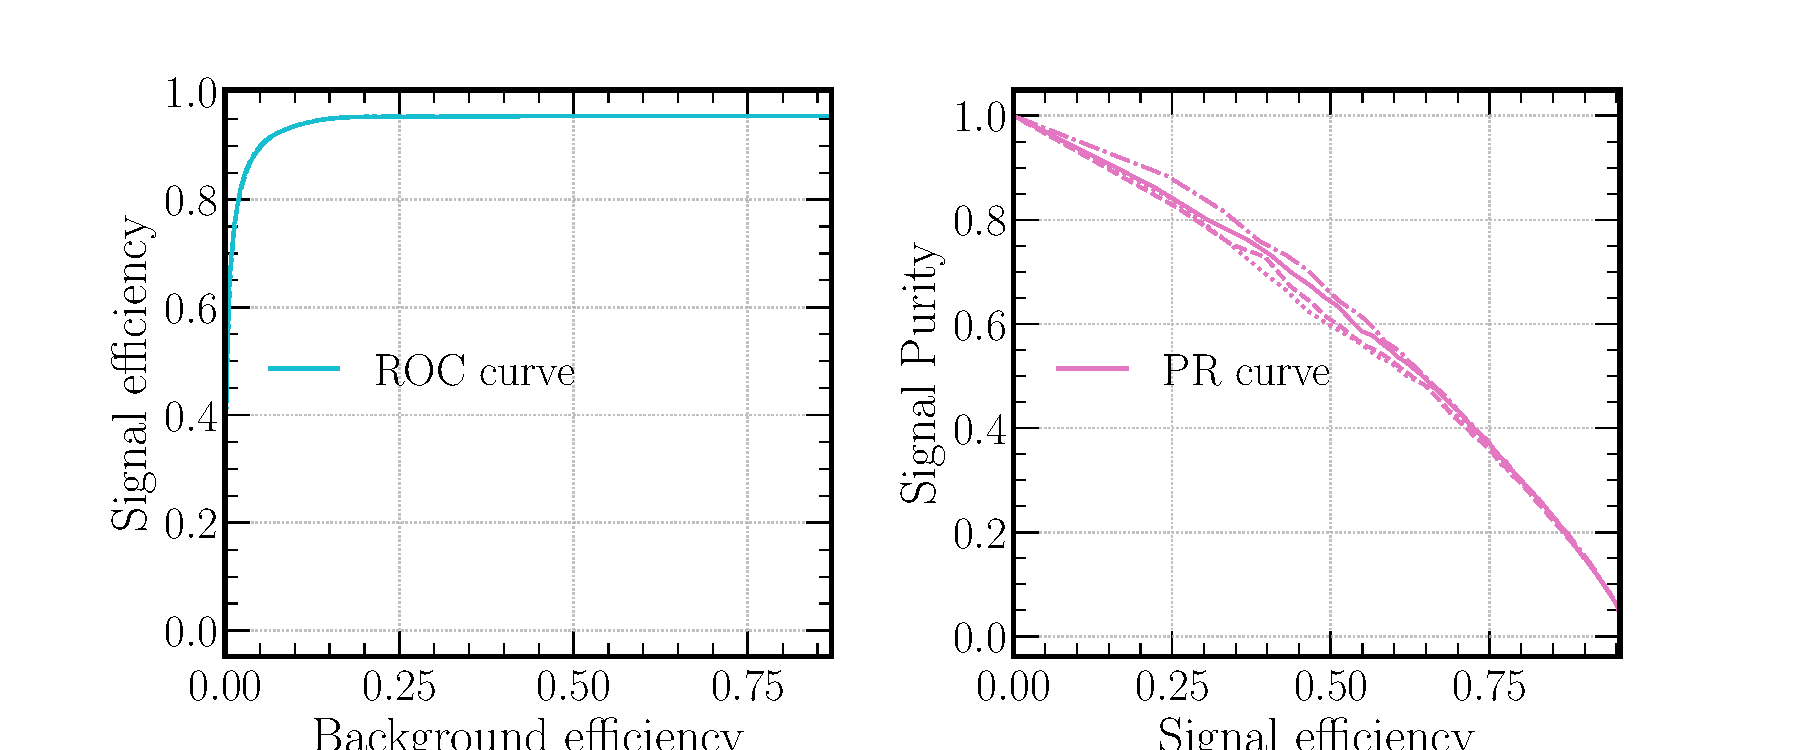
\includegraphics[width=0.8\textwidth]{diagrams/6-cvn/chipsnet/cat_nuel_comp_curves.pdf}
    \caption[cat nuel comp curves short]
    {cat nuel comp curves long}
    \label{fig:cat_nuel_comp_curves}
\end{figure}

\begin{figure} % CAT NUMU EFF CURVES DIAGRAM %
    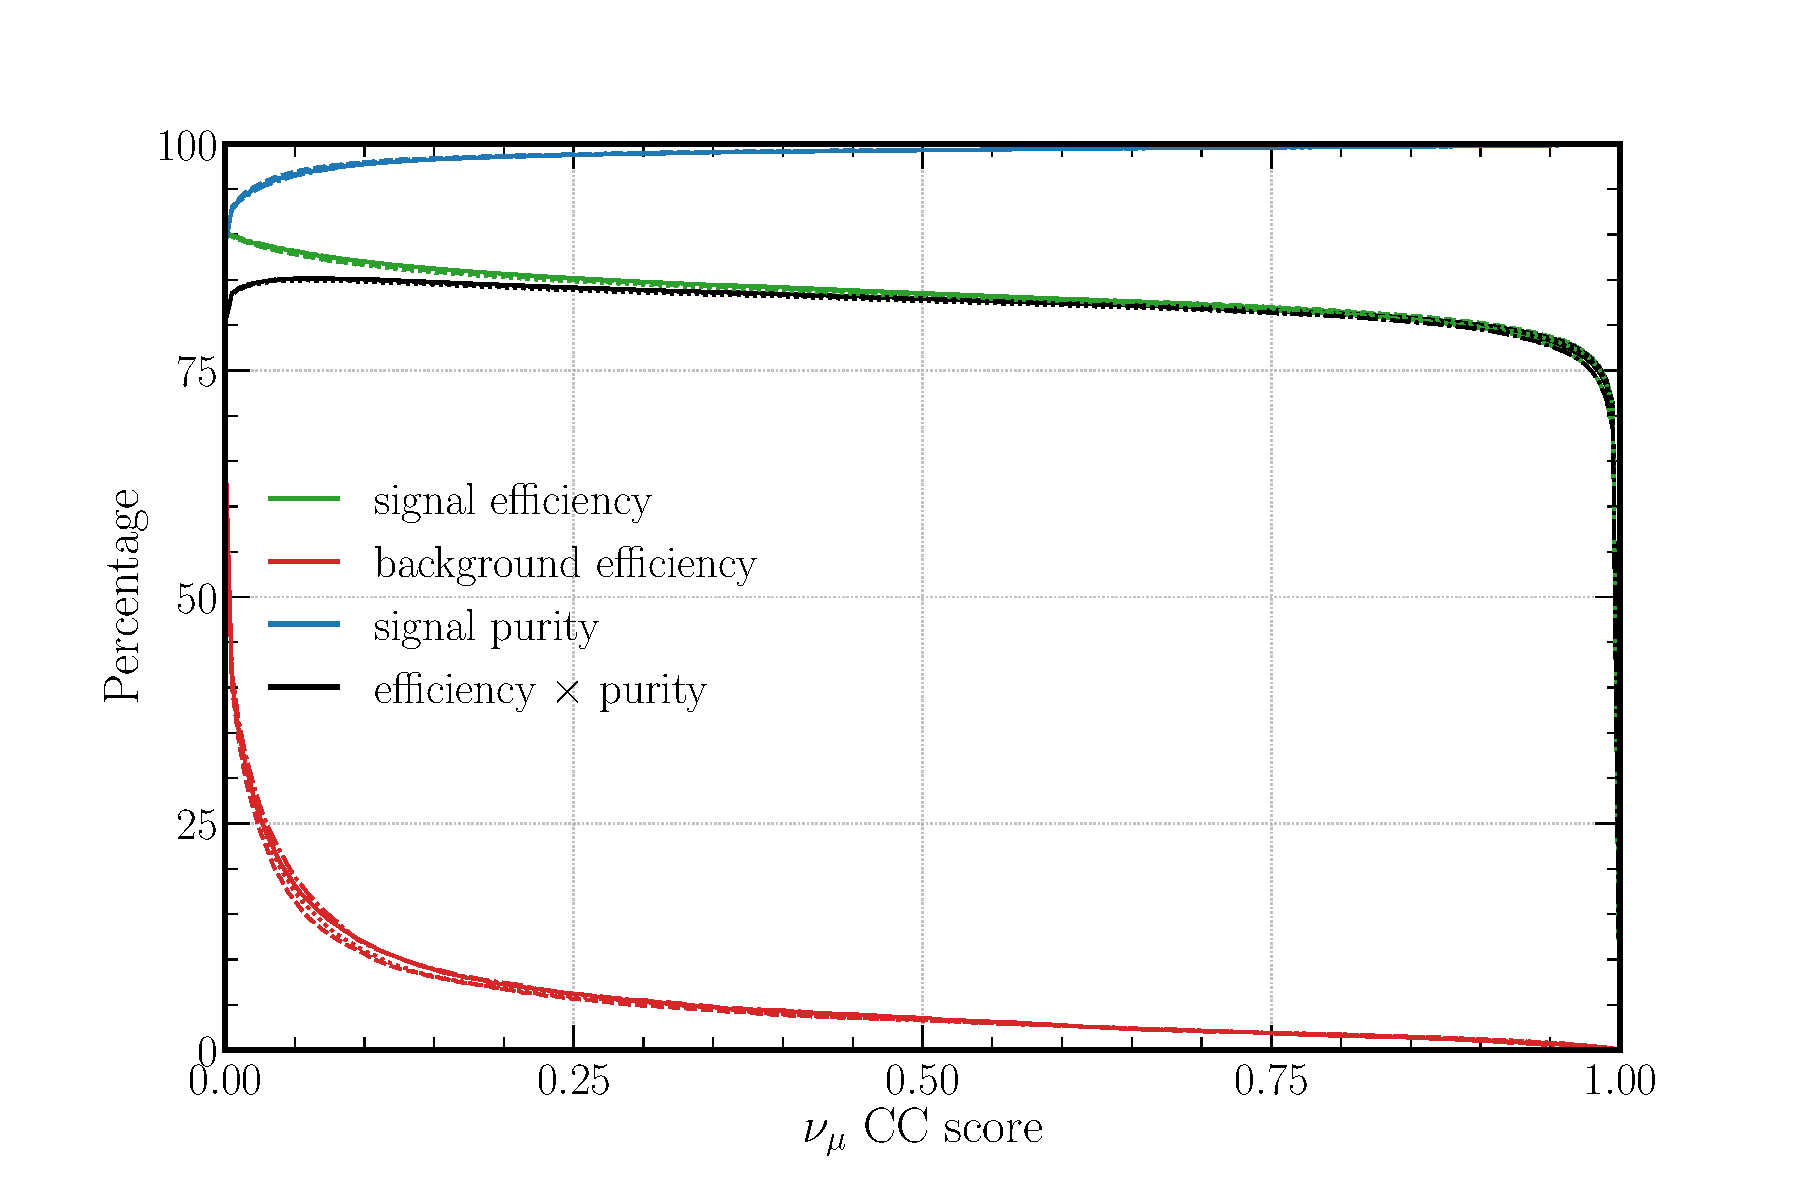
\includegraphics[width=0.6\textwidth]{diagrams/6-cvn/chipsnet/cat_numu_eff_curves.pdf}
    \caption[cat numu eff curves short]
    {cat numu eff curves long}
    \label{fig:cat_numu_eff_curves}
\end{figure}

\begin{figure} % CAT NUMU COMP CURVES DIAGRAM %
    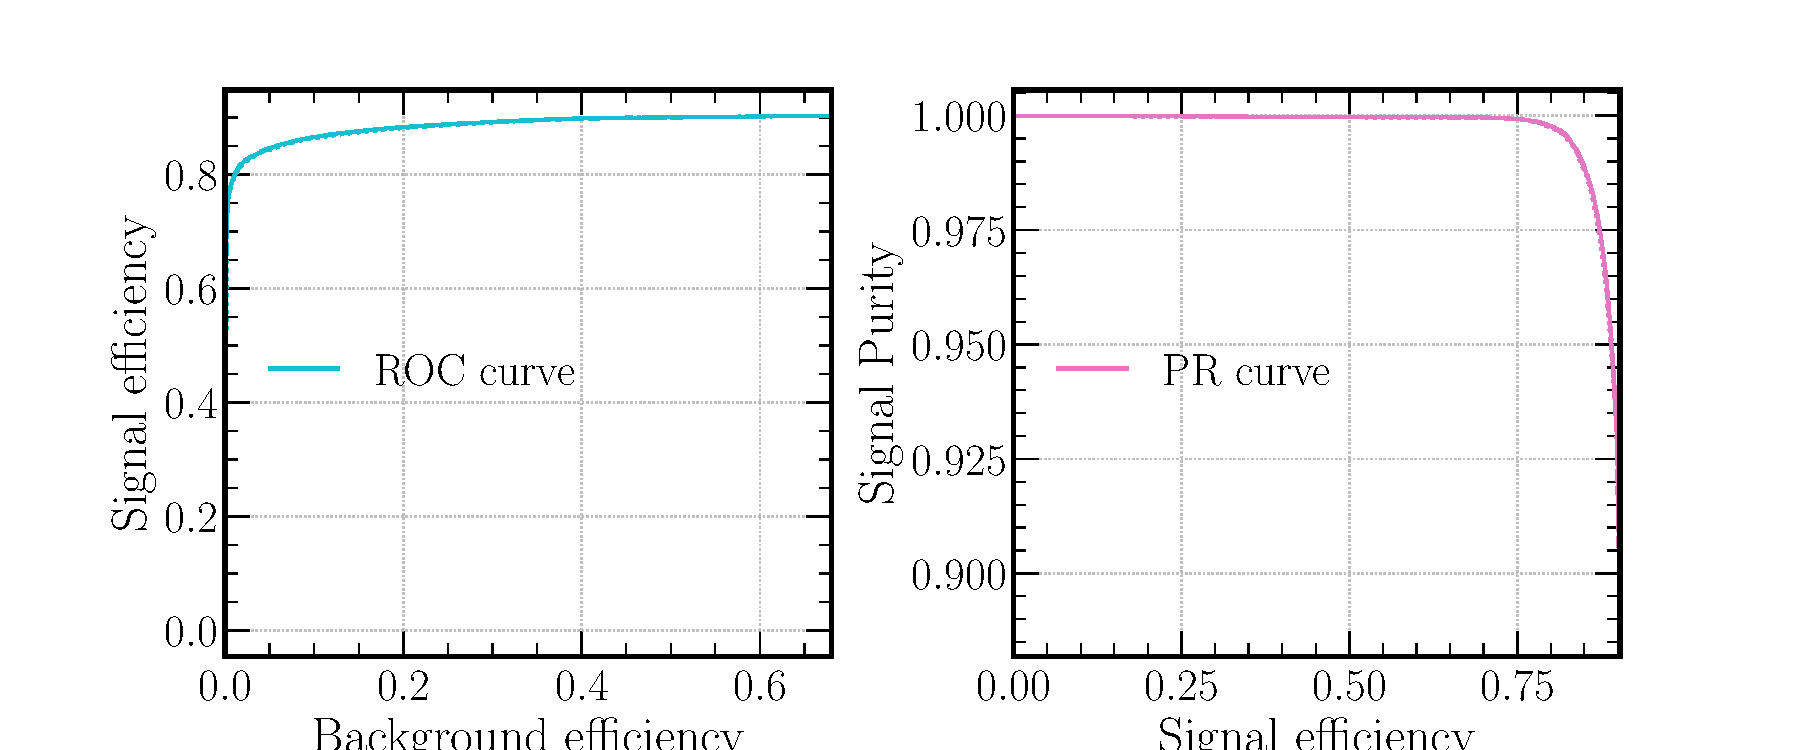
\includegraphics[width=0.8\textwidth]{diagrams/6-cvn/chipsnet/cat_numu_comp_curves.pdf}
    \caption[cat numu comp curves short]
    {cat numu comp curves long}
    \label{fig:cat_numu_comp_curves}
\end{figure}

\subsection{Does counting primary particles help?} %%%%%%%%%%%%%%%%%%%%%%%%%%%%%%%%%%%%%%%%%%%%%%%
\label{sec:cvn_beam_prim} %%%%%%%%%%%%%%%%%%%%%%%%%%%%%%%%%%%%%%%%%%%%%%%%%%%%%%%%%%%%%%%%%%%%%%%%

- DUne tried counting exclusive final state particles (protons, chargedpions, neutral pions)
- As the different final states will have different energy resolutions and sytematic
uncertainties, it may be possible for a future analysis to improve the oscillation paramter
sensitivity by indentifying subsamples with specific topologies.
- Primary partile scores can be combined to give compounded scores for the exclusive final state
selections.

\begin{figure} % BEAM NUEL EFF CURVES DIAGRAM %
    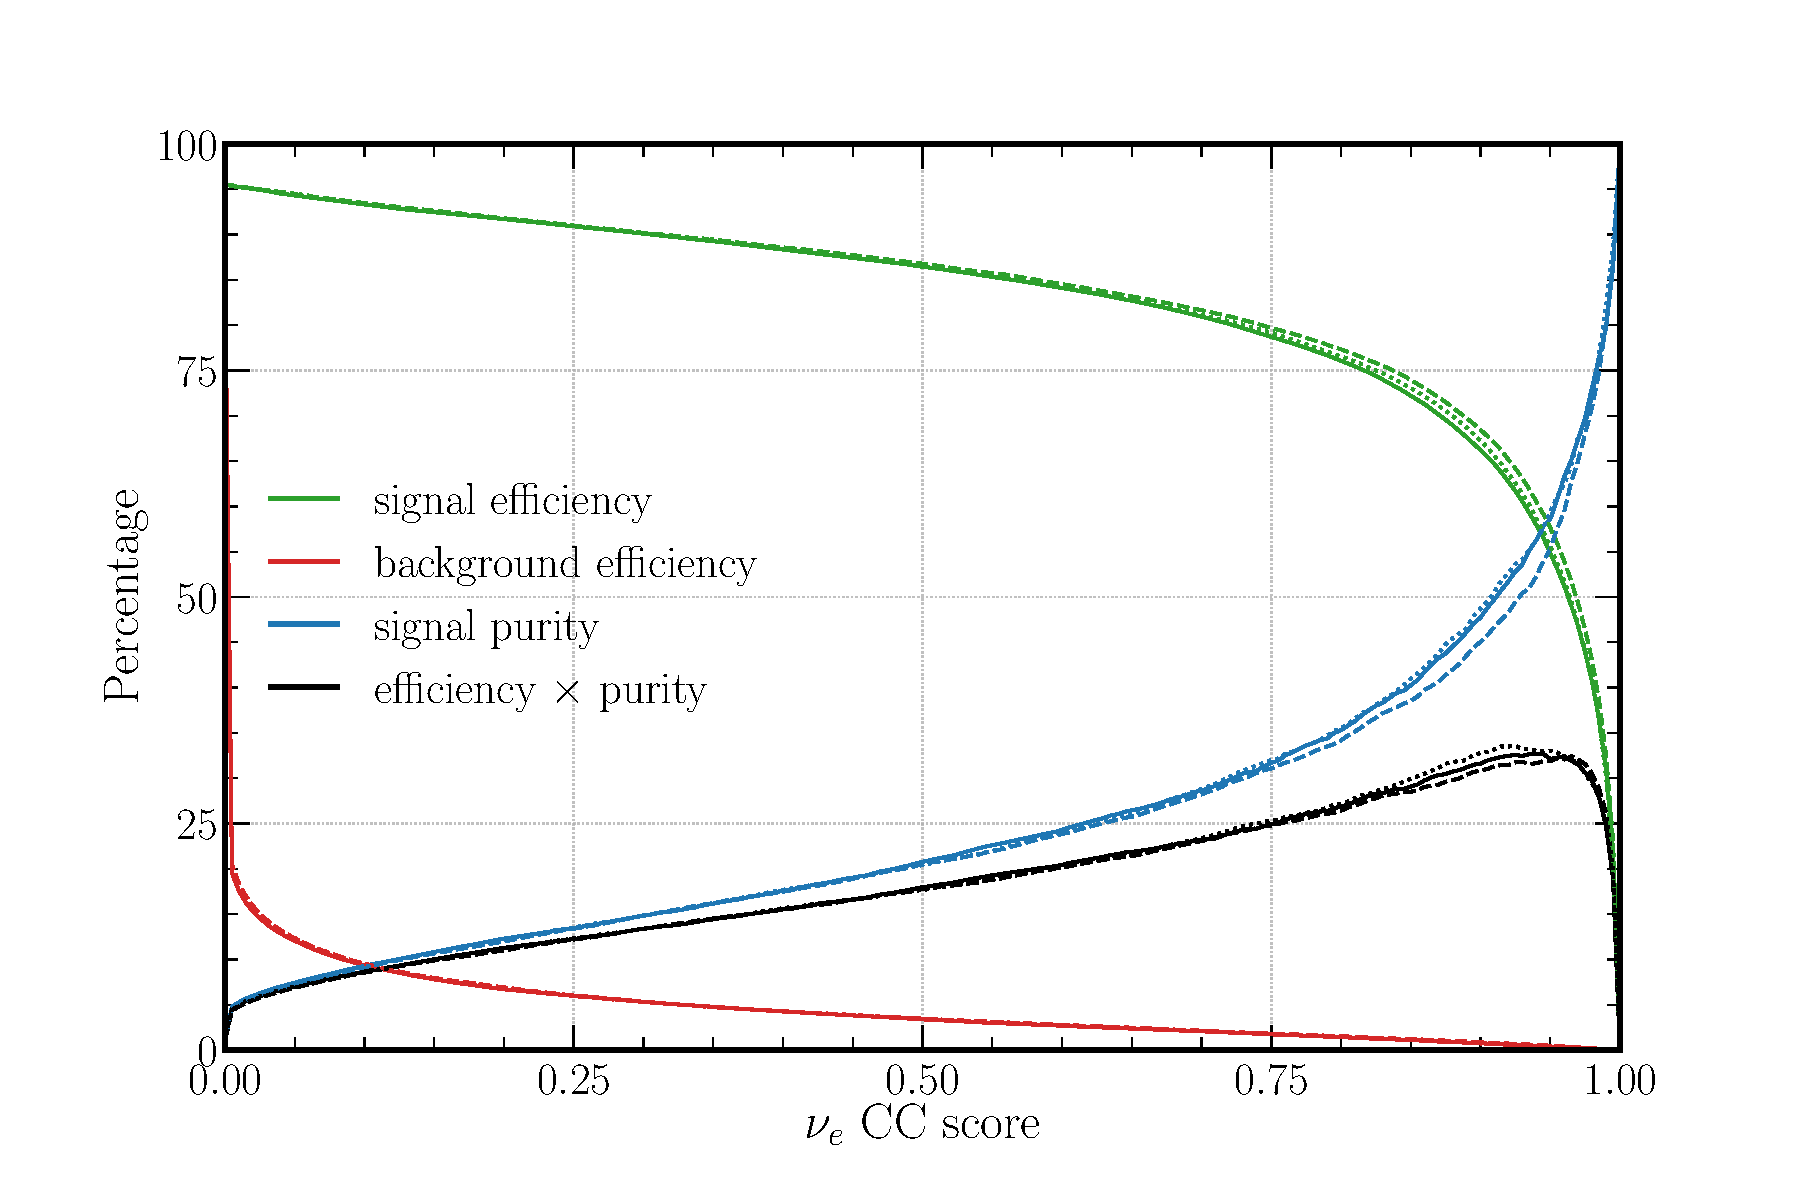
\includegraphics[width=0.6\textwidth]{diagrams/6-cvn/chipsnet/beam_nuel_eff_curves.pdf}
    \caption[beam nuel eff curves short]
    {beam nuel eff curves long}
    \label{fig:beam_nuel_eff_curves}
\end{figure}

\begin{figure} % BEAM NUEL COMP CURVES DIAGRAM %
    \includegraphics[width=0.8\textwidth]{diagrams/6-cvn/chipsnet/beam_nuel_comp_curves.pdf}
    \caption[beam nuel comp curves short]
    {beam nuel comp curves long}
    \label{fig:beam_nuel_comp_curves}
\end{figure}

\begin{figure} % BEAM NUMU EFF CURVES DIAGRAM %
    \includegraphics[width=0.6\textwidth]{diagrams/6-cvn/chipsnet/beam_numu_eff_curves.pdf}
    \caption[beam numu eff curves short]
    {beam numu eff curves long}
    \label{fig:beam_numu_eff_curves}
\end{figure}

\begin{figure} % BEAM NUMU COMP CURVES DIAGRAM %
    \includegraphics[width=0.8\textwidth]{diagrams/6-cvn/chipsnet/beam_numu_comp_curves.pdf}
    \caption[beam numu comp curves short]
    {beam numu comp curves long}
    \label{fig:beam_numu_comp_curves}
\end{figure}

\section{Energy estimation} %%%%%%%%%%%%%%%%%%%%%%%%%%%%%%%%%%%%%%%%%%%%%%%%%%%%%%%%%%%%%%%%%%%%%%
\label{sec:cvn_energy} %%%%%%%%%%%%%%%%%%%%%%%%%%%%%%%%%%%%%%%%%%%%%%%%%%%%%%%%%%%%%%%%%%%%%%%%%%%

\subsection{Neutrino and lepton multitask} %%%%%%%%%%%%%%%%%%%%%%%%%%%%%%%%%%%%%%%%%%%%%%%%%%%%%%%
\label{sec:cvn_energy_chan} %%%%%%%%%%%%%%%%%%%%%%%%%%%%%%%%%%%%%%%%%%%%%%%%%%%%%%%%%%%%%%%%%%%%%%

\begin{figure} % ENERGY CHAN DISTS DIAGRAM %
    \includegraphics[width=\textwidth]{diagrams/6-cvn/chipsnet/energy_chan_frac_dist.pdf}
    \caption[energy chan frac dist short]
    {energy chan frac dist long}
    \label{fig:energy_chan_frac_dist}
\end{figure}

\begin{figure} % ENERGY CHAN FRAC VS E DIAGRAM %
    \includegraphics[width=\textwidth]{diagrams/6-cvn/chipsnet/energy_chan_frac_vs_e.pdf}
    \caption[energy chan frac vs e short]
    {energy chan frac vs e long}
    \label{fig:energy_chan_frac_vs_e}
\end{figure}

\subsection{Extra parameters} %%%%%%%%%%%%%%%%%%%%%%%%%%%%%%%%%%%%%%%%%%%%%%%%%%%%%%%%%%%%%%%%%%%%
\label{sec:cvn_energy_par} %%%%%%%%%%%%%%%%%%%%%%%%%%%%%%%%%%%%%%%%%%%%%%%%%%%%%%%%%%%%%%%%%%%%%%%

\begin{figure} % ENERGY PAR DISTS DIAGRAM %
    \includegraphics[width=\textwidth]{diagrams/6-cvn/chipsnet/energy_par_frac_dist.pdf}
    \caption[energy par frac dist short]
    {energy par frac dist long}
    \label{fig:energy_par_frac_dist}
\end{figure}

\begin{figure} % ENERGY PAR FRAC VS E DIAGRAM %
    \includegraphics[width=\textwidth]{diagrams/6-cvn/chipsnet/energy_par_frac_vs_e.pdf}
    \caption[energy par frac vs e short]
    {energy par frac vs e long}
    \label{fig:energy_par_frac_vs_e}
\end{figure}

\subsection{Combined or split} %%%%%%%%%%%%%%%%%%%%%%%%%%%%%%%%%%%%%%%%%%%%%%%%%%%%%%%%%%%%%%%%%%%
\label{sec:cvn_energy_split} %%%%%%%%%%%%%%%%%%%%%%%%%%%%%%%%%%%%%%%%%%%%%%%%%%%%%%%%%%%%%%%%%%%%%

\begin{figure} % ENERGY SPLIT NUEL DIAGRAM %
    \includegraphics[width=\textwidth]{diagrams/6-cvn/chipsnet/final_energy_split_nuel_frac_vs_e.pdf}
    \caption[final energy split nuel frac vs e short]
    {final energy split nuel frac vs e long}
    \label{fig:final_energy_split_nuel_frac_vs_e}
\end{figure}

\begin{figure} % ENERGY SPLIT NUMU DIAGRAM %
    \includegraphics[width=\textwidth]{diagrams/6-cvn/chipsnet/final_energy_split_numu_frac_vs_e.pdf}
    \caption[final energy split numu frac vs e short]
    {final energy split numu frac vs e long}
    \label{fig:final_energy_split_numu_frac_vs_e}
\end{figure}

\section{Combined performance} %%%%%%%%%%%%%%%%%%%%%%%%%%%%%%%%%%%%%%%%%%%%%%%%%%%%%%%%%%%%%%%%%%%
\label{sec:cvn_final} %%%%%%%%%%%%%%%%%%%%%%%%%%%%%%%%%%%%%%%%%%%%%%%%%%%%%%%%%%%%%%%%%%%%%%%%%%%%

\subsection{Comparison with standard methods} %%%%%%%%%%%%%%%%%%%%%%%%%%%%%%%%%%%%%%%%%%%%%%%%%%%%
\label{sec:cvn_final_comparison} %%%%%%%%%%%%%%%%%%%%%%%%%%%%%%%%%%%%%%%%%%%%%%%%%%%%%%%%%%%%%%%%%

\begin{figure} % COSMIC HISTORY DIAGRAM %
    \includegraphics[width=0.6\textwidth]{diagrams/6-cvn/chipsnet/final_cosmic_history.pdf}
    \caption[final cosmic history short]
    {final cosmic history long}
    \label{fig:final_cosmic_history}
\end{figure}

\begin{figure} % BEAM HISTORY DIAGRAM %
    \includegraphics[width=0.6\textwidth]{diagrams/6-cvn/chipsnet/final_beam_history.pdf}
    \caption[final beam history short]
    {final beam history long}
    \label{fig:final_beam_history}
\end{figure}

\begin{figure} % ENERGY HISTORY DIAGRAM %
    \includegraphics[width=0.6\textwidth]{diagrams/6-cvn/chipsnet/final_energy_history.pdf}
    \caption[final energy history short]
    {final energy history long}
    \label{fig:final_energy_history}
\end{figure}

\begin{figure} % COSMIC OUTPUTS DIAGRAM %
    \includegraphics[width=0.6\textwidth]{diagrams/6-cvn/chipsnet/final_cosmic_outputs.pdf}
    \caption[final cosmic outputs short]
    {final cosmic outputs long}
    \label{fig:final_cosmic_outputs}
\end{figure}

\begin{figure} % COSMIC OUTPUTS ZOOMED DIAGRAM %
    \includegraphics[width=0.6\textwidth]{diagrams/6-cvn/chipsnet/final_cosmic_zoomed_outputs.pdf}
    \caption[final cosmic zoomed outputs short]
    {final cosmic zoomed outputs long}
    \label{fig:final_cosmic_zoomed_outputs}
\end{figure}

\begin{figure} % ESCAPES OUTPUTS DIAGRAM %
    \includegraphics[width=0.6\textwidth]{diagrams/6-cvn/chipsnet/final_escapes_outputs.pdf}
    \caption[final escapes outputs short]
    {final escapes outputs long}
    \label{fig:final_escapes_outputs}
\end{figure}

\begin{figure} % BEAM OUTPUTS NUEL DIAGRAM %
    \includegraphics[width=0.6\textwidth]{diagrams/6-cvn/chipsnet/final_beam_nuel_outputs.pdf}
    \caption[final beam nuel outputs short]
    {final beam nuel outputs long}
    \label{fig:final_beam_nuel_outputs}
\end{figure}

\begin{figure} % BEAM OUTPUTS NUMU DIAGRAM %
    \includegraphics[width=0.6\textwidth]{diagrams/6-cvn/chipsnet/final_beam_numu_outputs.pdf}
    \caption[final beam numu outputs short]
    {final beam numu outputs long}
    \label{fig:final_beam_numu_outputs}
\end{figure}

\begin{figure} % FINAL NUEL EFF CURVES DIAGRAM %
    \includegraphics[width=0.6\textwidth]{diagrams/6-cvn/chipsnet/final_nuel_eff_curves.pdf}
    \caption[final nuel eff curves short]
    {final nuel eff curves long}
    \label{fig:final_nuel_eff_curves}
\end{figure}

\begin{figure} % FINAL NUMU EFF CURVES DIAGRAM %
    \includegraphics[width=0.6\textwidth]{diagrams/6-cvn/chipsnet/final_numu_eff_curves.pdf}
    \caption[final numu eff curves short]
    {final numu eff curves long}
    \label{fig:final_numu_eff_curves}
\end{figure}

\begin{figure} % FINAL NUEL HISTS DIAGRAM %
    \includegraphics[width=0.6\textwidth]{diagrams/6-cvn/chipsnet/final_nuel_hists.pdf}
    \caption[final nuel hists short]
    {final nuel hists long}
    \label{fig:final_nuel_hists}
\end{figure}

\begin{figure} % FINAL NUMU HISTS DIAGRAM %
    \includegraphics[width=0.6\textwidth]{diagrams/6-cvn/chipsnet/final_numu_hists.pdf}
    \caption[final numu hists short]
    {final numu hists long}
    \label{fig:final_numu_hists}
\end{figure}

\begin{figure} % FINAL COMB CAT CONFUSION DIAGRAM %
    \includegraphics[width=0.6\textwidth]{diagrams/6-cvn/chipsnet/final_comb_cat_confusion.pdf}
    \caption[final comb cat confusion short]
    {final comb cat confusion long}
    \label{fig:final_comb_cat_confusion}
\end{figure}

\begin{figure} % FINAL CC CAT CONFUSION DIAGRAM %
    \includegraphics[width=0.6\textwidth]{diagrams/6-cvn/chipsnet/final_cc_cat_confusion.pdf}
    \caption[final cc cat confusion short]
    {final cc cat confusion long}
    \label{fig:final_cc_cat_confusion}
\end{figure}

\begin{figure} % FINAL NC CAT CONFUSION DIAGRAM %
    \includegraphics[width=0.6\textwidth]{diagrams/6-cvn/chipsnet/final_nc_cat_confusion.pdf}
    \caption[final nc cat confusion short]
    {final nc cat confusion long}
    \label{fig:final_nc_cat_confusion}
\end{figure}

\begin{figure} % FINAL NUEL ENERGY DIST DIAGRAM %
    \includegraphics[width=0.6\textwidth]{diagrams/6-cvn/chipsnet/final_nuel_passed_energy_dist.pdf}
    \caption[final nuel passed energy dist short]
    {final nuel passed energy dist long}
    \label{fig:final_nuel_passed_energy_dist}
\end{figure}

\begin{figure} % FINAL NUMU ENERGY DIST DIAGRAM %
    \includegraphics[width=0.6\textwidth]{diagrams/6-cvn/chipsnet/final_numu_passed_energy_dist.pdf}
    \caption[final numu passed energy dist short]
    {final numu passed energy dist long}
    \label{fig:final_numu_passed_energy_dist}
\end{figure}

\begin{figure} % FINAL 2D ENERGY DIAGRAM %
    \includegraphics[width=0.7\textwidth]{diagrams/6-cvn/chipsnet/final_energy_2d.pdf}
    \caption[final energy 2d short]
    {final energy 2d long}
    \label{fig:final_energy_2d}
\end{figure}

\begin{figure} % FINAL NUEL ENERGY DIAGRAM %
    \includegraphics[width=0.8\textwidth]{diagrams/6-cvn/chipsnet/final_energy_nuel.pdf}
    \caption[final energy nuel short]
    {final energy nuel long}
    \label{fig:final_energy_nuel}
\end{figure}

\begin{figure} % FINAL NUMU ENERGY DIAGRAM %
    \includegraphics[width=0.8\textwidth]{diagrams/6-cvn/chipsnet/final_energy_numu.pdf}
    \caption[final energy numu short]
    {final energy numu long}
    \label{fig:final_energy_numu}
\end{figure}

DIAGRAM: True neutrino energy distributions for different categories for energy estimation.
DIAGRAM: Neutrino energy and estimated neutrino energy distributions on same plots.
INFO: Table of the final number of expected events and efficiency and purity of the signal at the
chosen cut value (nuel and numu)
DIAGRAM: Parrallel coordinates plots for tuning the hyperparameters
INFO: Time taken comparison with old reconstruction (just inference time for all stages)
INFO: Super-k/Dune/Nova comparison numbers for effeciencies and energy resolutions etc...
DIAGRAM: Table of how succesive cuts affect the selection of different event types
DIAGRAM: Plots of exclusive state predictions by multiplying different score outputs.

- BIG UP the difference in time it takes, as this can have a huge impact on reprocessing your full
dataset
- This allows a massive increase in the iteration rate of analysis, which can lead to an improved
rate of improvement, with less time wasted.

INFO: Need to understand the error on the number of cosmic passing the cut, is it reasonable
without a huge amount of testing data?
INFO: What are the errors on all my number values? with the stats I have?
- Having a veto in the upstream towards the beam direction would be best
- Talk about how beam muons upstream of the detector are just like cosmics and say how they could
be rejected aswell
INFO: proof that there is no topological difference between QEL and MEC if we are combining them
for the energy stuff
- Position of PMTs does not seem to be that important

- Nova gets about ~7percent energy resolution for signal events
in Ref.~\cite{jiang2019}
- Fitqun gets ~20cm vertex position resolution for nuel CCQE events
- Fitqun gets ~16cm vertex position resolution for numu CCQE events
- Fitqun gets 5.39percent to 2.58percent lepton energy resolution for nuel CCQE events
- Fitqun gets ~2.5percent lepton energy resolution for numu CCQE events
- Note all the stuff in super-k happens at lower energies ~<1.4GeV

\section{Explainability} %%%%%%%%%%%%%%%%%%%%%%%%%%%%%%%%%%%%%%%%%%%%%%%%%%%%%%%%%%%%%%%%%%%%%%%%%
\label{sec:cvn_explain} %%%%%%%%%%%%%%%%%%%%%%%%%%%%%%%%%%%%%%%%%%%%%%%%%%%%%%%%%%%%%%%%%%%%%%%%%%

\begin{figure} % COSMIC t-SNE DIAGRAM %
    \includegraphics[width=0.8\textwidth]{diagrams/6-cvn/chipsnet/final_cosmic_tsne.pdf}
    \caption[final cosmic tsne short]
    {final cosmic tsne long}
    \label{fig:final_cosmic_tsne}
\end{figure}

\begin{figure} % BEAM t-SNE DIAGRAM %
    \includegraphics[width=0.8\textwidth]{diagrams/6-cvn/chipsnet/final_beam_tsne.pdf}
    \caption[final beam tsne short]
    {final beam tsne long}
    \label{fig:final_beam_tsne}
\end{figure}

\begin{figure} % BEAM t-SNE EVENTS DIAGRAM %
    \includegraphics[width=\textwidth]{diagrams/6-cvn/chipsnet/final_beam_tsne_events.pdf}
    \caption[final beam tsne events short]
    {final beam tsne events long}
    \label{fig:final_beam_tsne_events}
\end{figure}

\begin{figure} % FRAC ENERGY EFF DIAGRAM %
    \includegraphics[width=0.6\textwidth]{diagrams/6-cvn/chipsnet/final_frac_energy_eff.pdf}
    \caption[final frac energy eff short]
    {final frac energy eff long}
    \label{fig:final_frac_energy_eff}
\end{figure}

\begin{figure} % EXPLAIN EXAMPLE EVENT DIAGRAM %
    \includegraphics[width=\textwidth]{diagrams/6-cvn/chipsnet/explain_example_event.pdf}
    \caption[explain example event short]
    {explain example event long}
    \label{fig:explain_example_event}
\end{figure}

\begin{figure} % BEAGLEBONE AND DANOUT DIAGRAM %
    \centering
    \subcaptionbox{explain cosmic activations\label{fig:explain_cosmic_activations}}{%
        \includegraphics[height=16cm]{diagrams/6-cvn/chipsnet/explain_cosmic_activations.pdf}%
    }
    \quad
    \subcaptionbox{explain beam activations\label{fig:explain_beam_activations}}{%
        \includegraphics[height=16cm]{diagrams/6-cvn/chipsnet/explain_beam_activations.pdf}%
    }
    \quad
    \subcaptionbox{explain energy activations\label{fig:explain_energy_activations}}{%
        \includegraphics[height=16cm]{diagrams/6-cvn/chipsnet/explain_energy_activations.pdf}%
    }
    \caption[The caption]
    {The caption}
\end{figure}

Initial CNN visualisation paper in Ref.~\cite{zeiler2013}
Original t-SNE paper in Ref.~\cite{maaten2008}
Grad-CAM paper in Ref.~\cite{selvaraju2017}

- For all the t-SNE stuff
- There have been plently of attempts at visualising high-dimensional data on a 2/3 dimensional
map, including Sammon mapping, Isomap, Locally Linear Embedding, Stochastic Neighbour Embedding.
- Older implementations tended to cluster all data points towards the centre of the map and proved
difficult to optimise.
- You basically set a summed probability between all points in the low-dimensional space to a
summed probability between all points in the high-dimensional space.
- t-SNE uses the student-t distribution (with a heavy tail) in the low-dimensional space to
calculate the probability. This alleviates both the crowding problem and is easier to optimise.
- Optimisation uses a simple momentum term, plus two new ideas. "Early compression" which forces
map points to stay close to each other at the start of optimisation, it is then easier for
clusters to move through each other and explore all possible global organisations of the data,
this is implemented as an L2-penalty term proportional to the sum of squared distances from the
origin, this is then removed at an iteration given as input. Secondly, "Early exaggeration" which
creates tight widely seperated clusters.